\documentclass[14pt, a4paper]{book}
\begin{document}\label{chap:Best_ML}
Something something Time to prepare our ML algorithms, statistics etc..

\chapter{Model dependent approach}
Now that we have established what type of ML network we will utilze as well as optimizig everything such that ... \todo{write more}

\section{The datasets}
Do I need to explain it again if I have in on Table \ref{tab:dataset}

\newpage
\graphicspath{{../../../Plots/}}
\section{Dark Higgs Heavy Dark Sector}
Trained a network using all of the SM background samples and every different Z' mass of this model. Here are the results
\begin{figure}[!ht]
	\centering
	\begin{subfigure}[b]{0.49\textwidth}
      \centering
      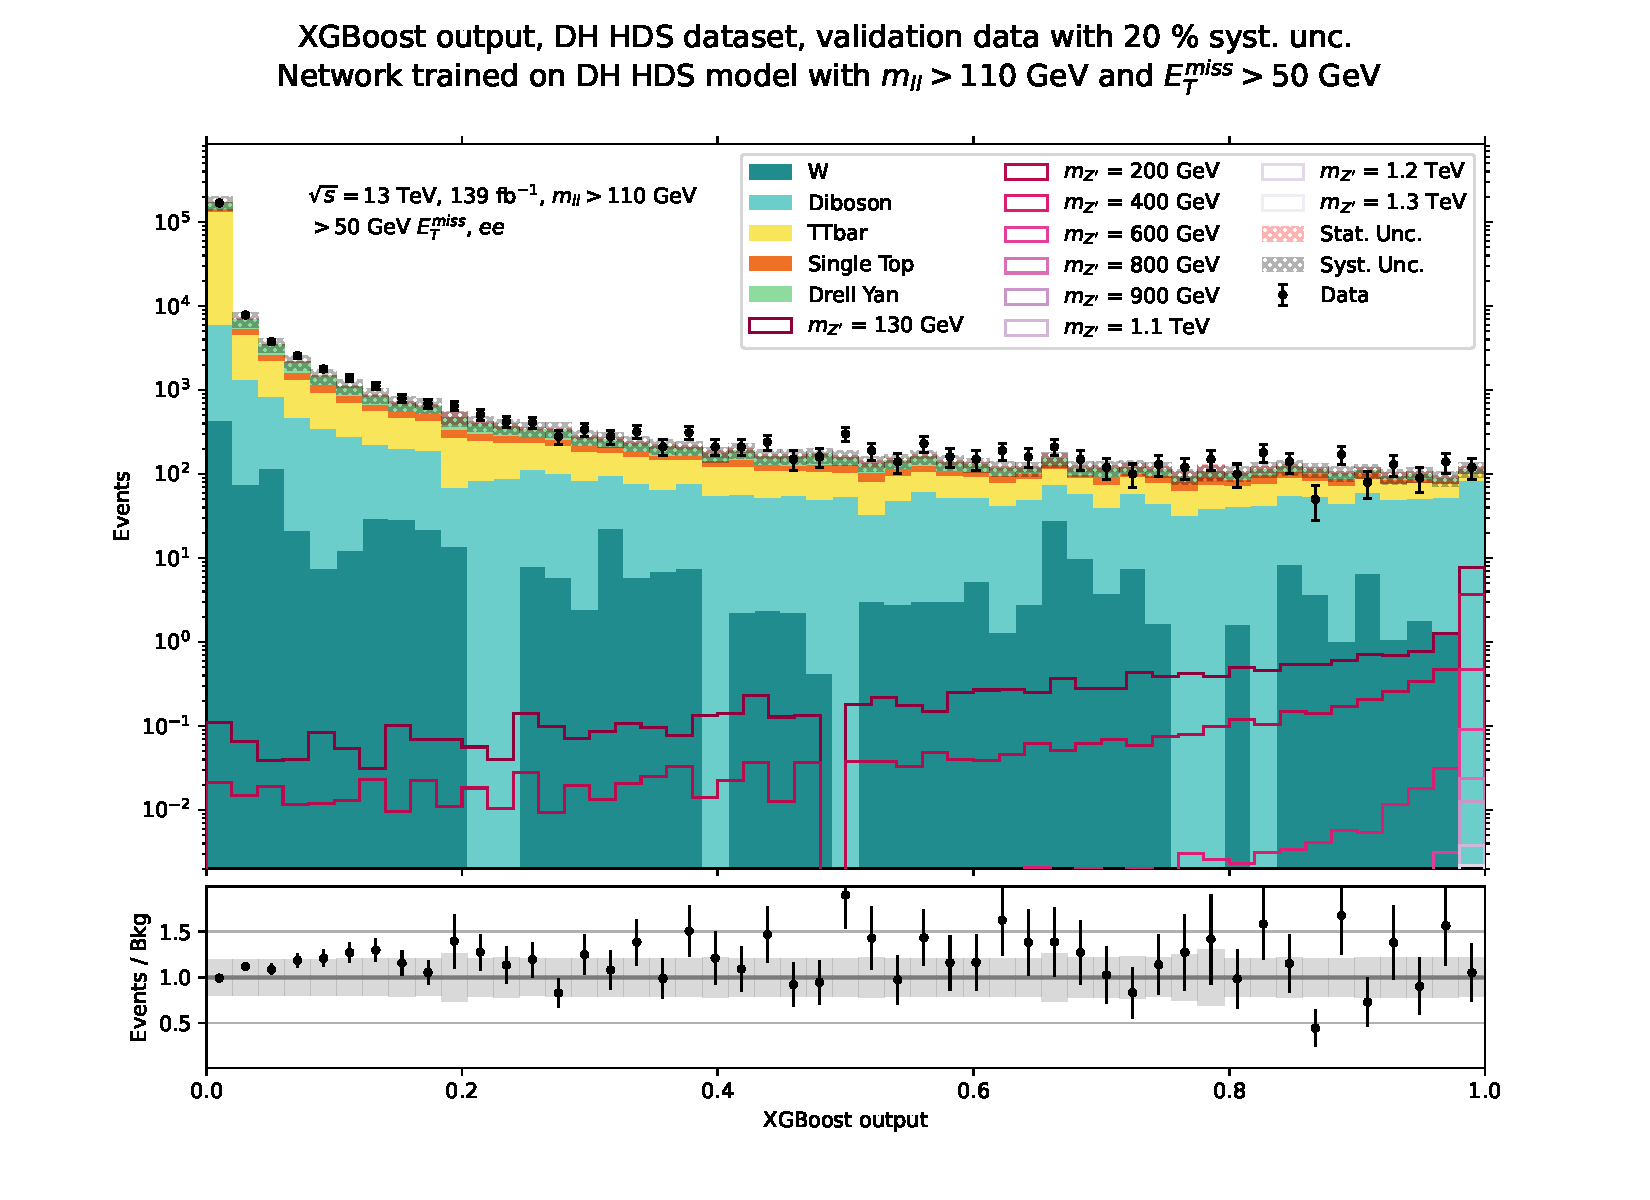
\includegraphics[width=1\textwidth]{XGBoost/DH_HDS/VAL_ee.pdf}
      \end{subfigure}
   \hfill
   \begin{subfigure}[b]{0.49\textwidth}
      \centering
      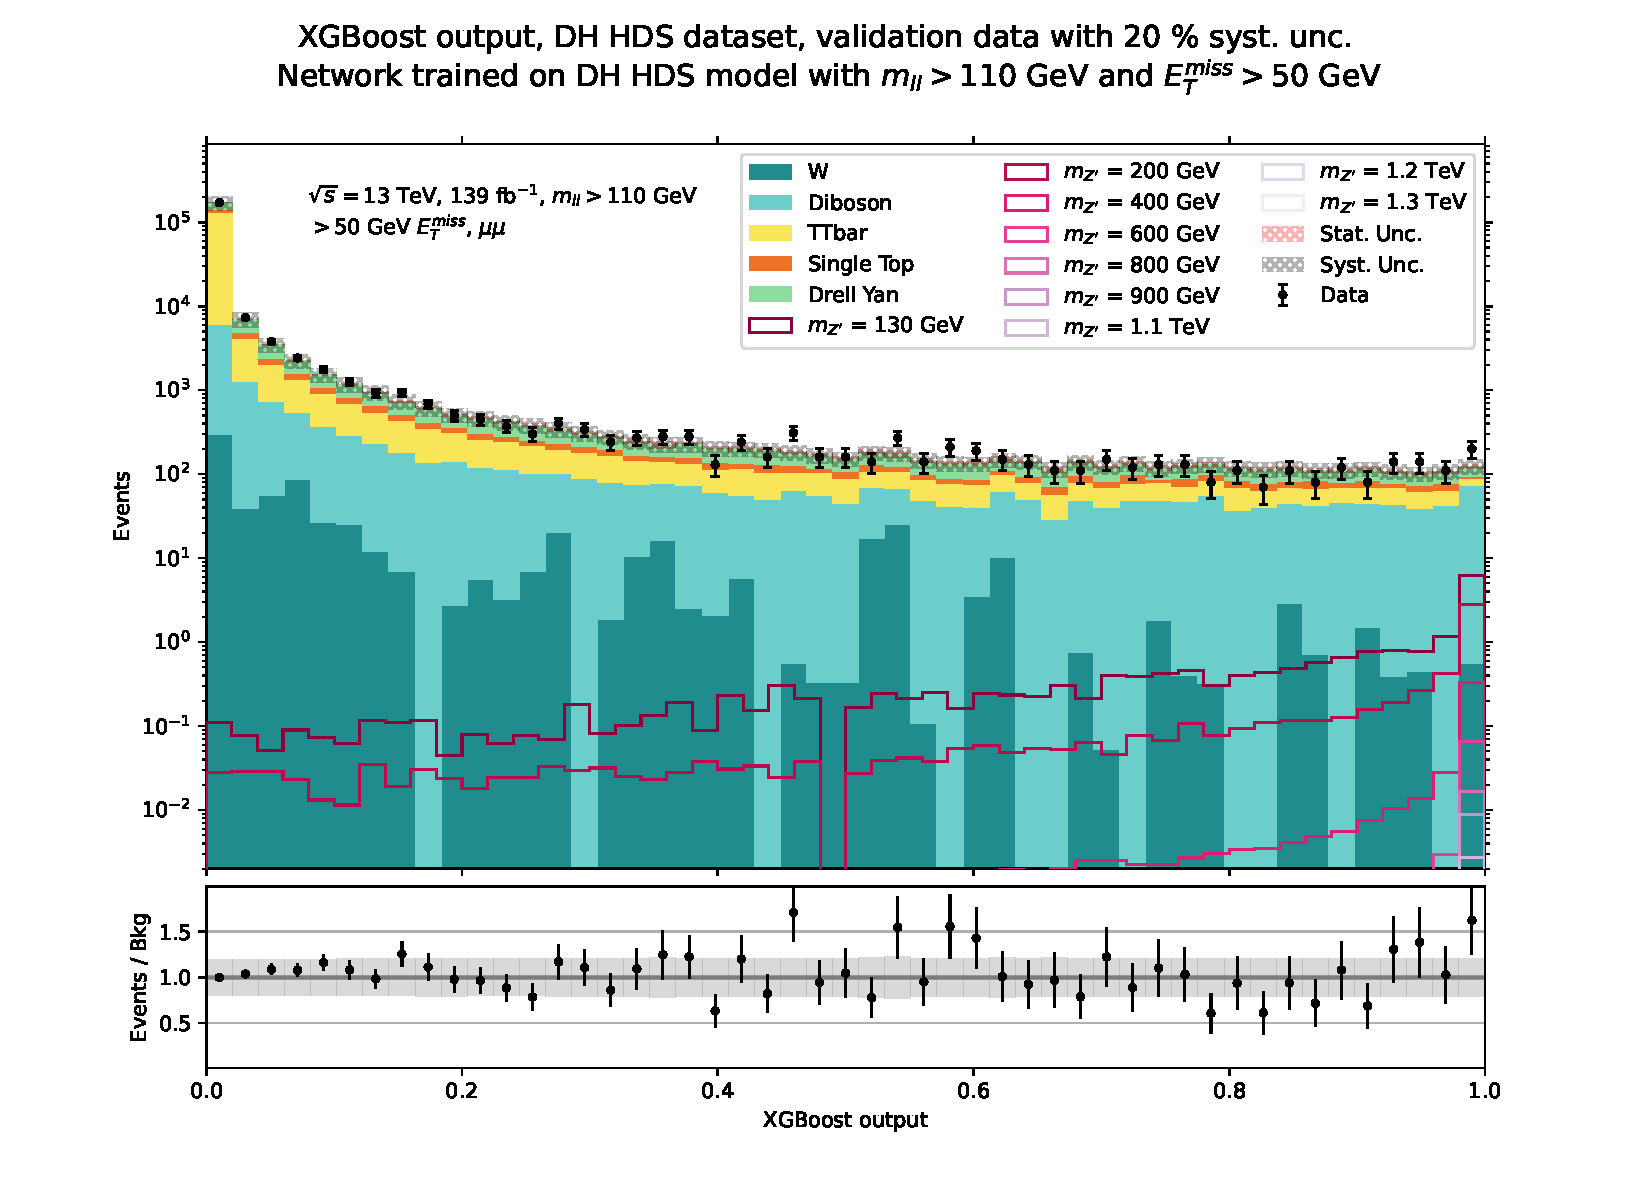
\includegraphics[width=1\textwidth]{XGBoost/DH_HDS/VAL_uu.pdf}
      \end{subfigure}
   \caption{Validation plots for network trained on Z' DH HDS}\label{fig:DH_HDS_vals}
\end{figure}
\\With the ROC for each mass point seen in Figure \ref{fig:DH_HDS_ROCS}.
\begin{figure}[!ht]
	\centering
	\begin{subfigure}[b]{0.49\textwidth}
      \centering
      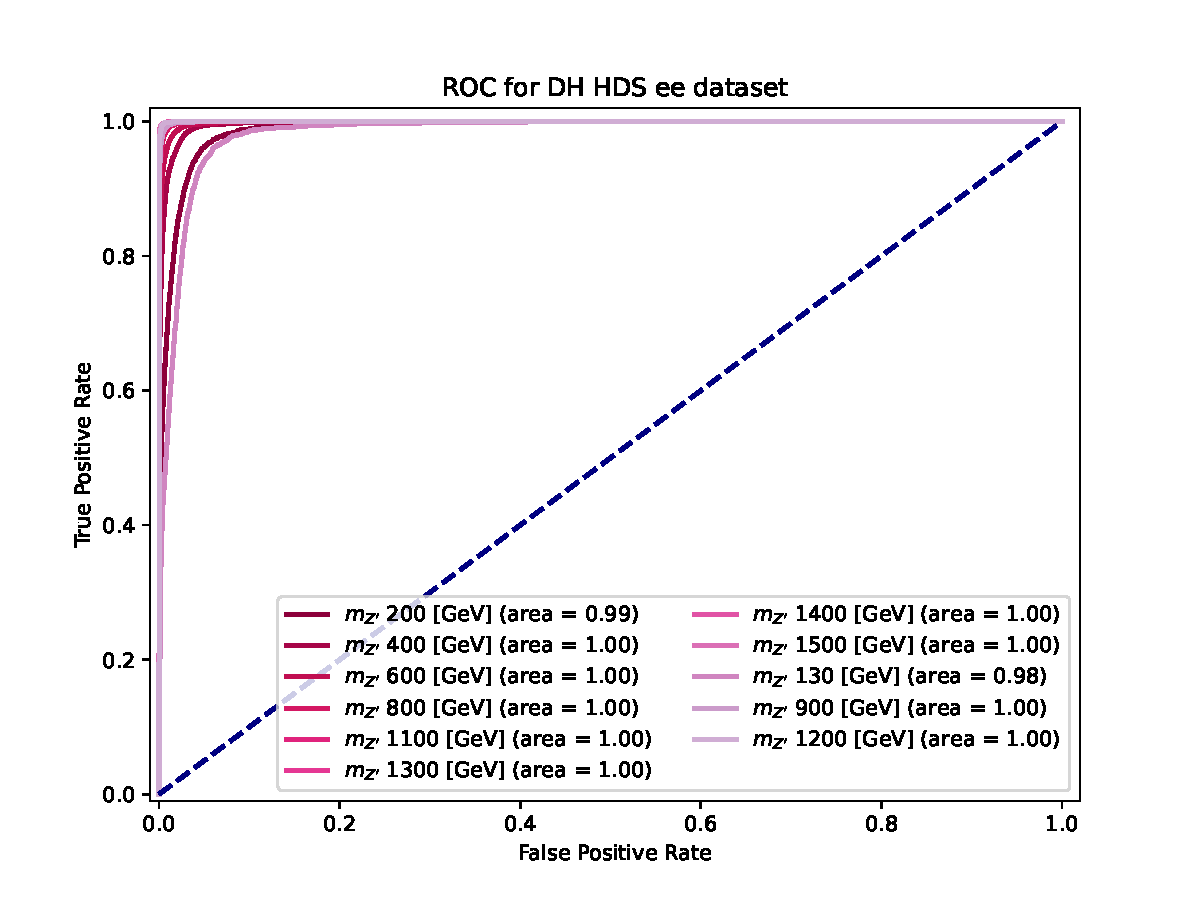
\includegraphics[width=1\textwidth]{XGBoost/DH_HDS/ROC_ee.pdf}
      \end{subfigure}
   \hfill
   \begin{subfigure}[b]{0.49\textwidth}
      \centering
      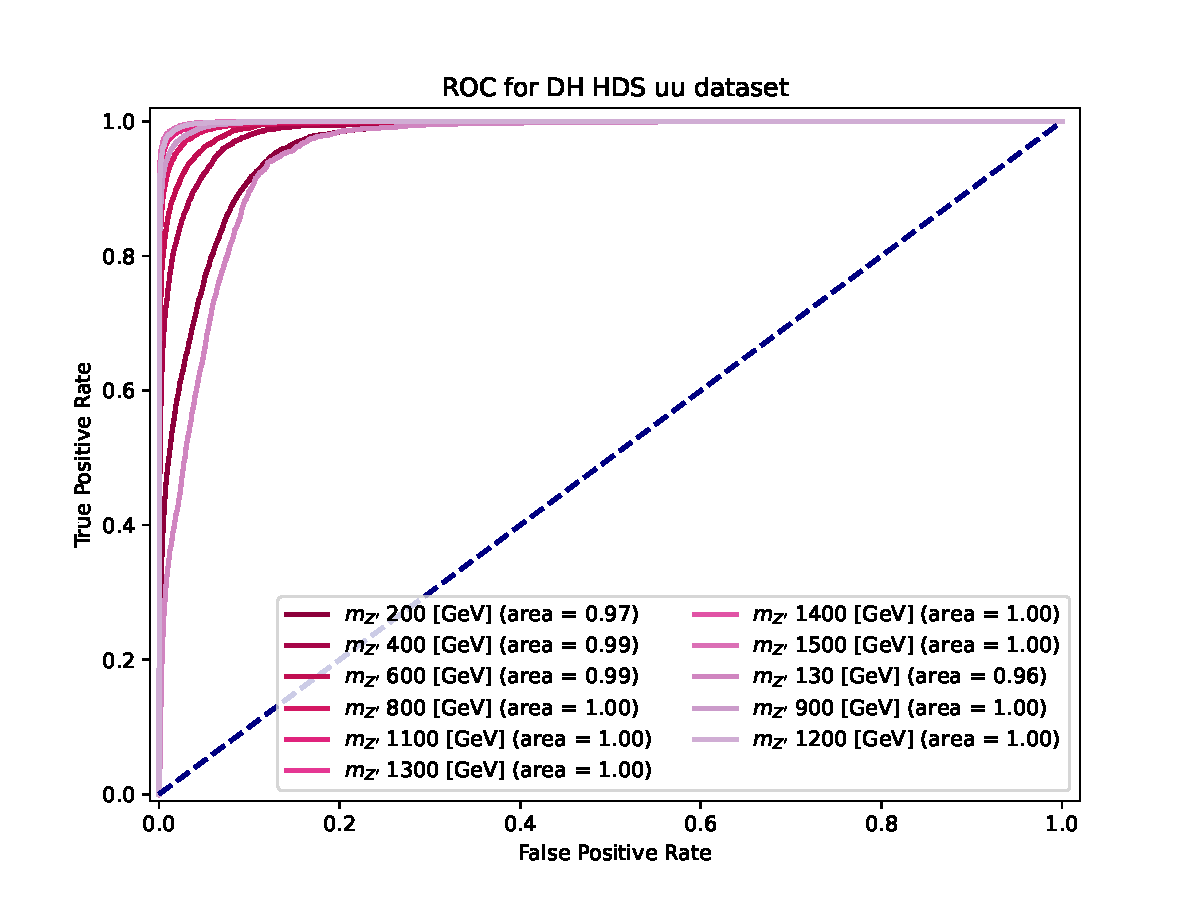
\includegraphics[width=1\textwidth]{XGBoost/DH_HDS/ROC_uu.pdf}
      \end{subfigure}
   \caption{ROC plots for every Z' mass point on network trained on Z' DH HDS}\label{fig:DH_HDS_ROCS}
\end{figure}
\\Plotting the significance of the models given the binning we get the results from Figure \ref{fig:DH_HDS_exp_sig}
\begin{figure}[!ht]
	\centering
	\begin{subfigure}[b]{0.49\textwidth}
      \centering
      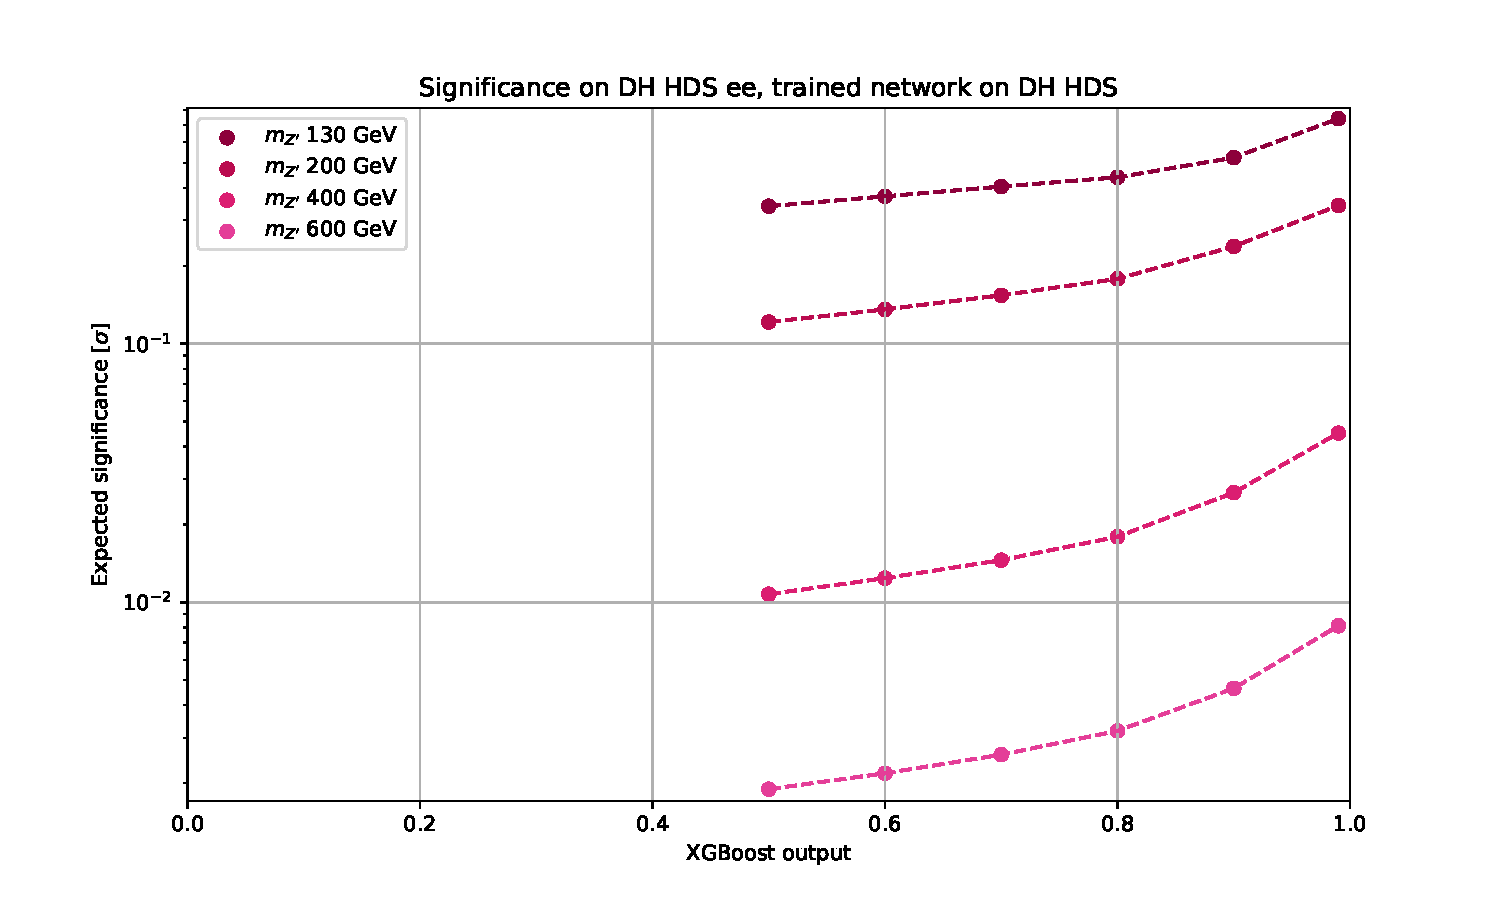
\includegraphics[width=1\textwidth]{XGBoost/DH_HDS/EXP_SIG_ee.pdf}
      \end{subfigure}
   \hfill
   \begin{subfigure}[b]{0.49\textwidth}
      \centering
      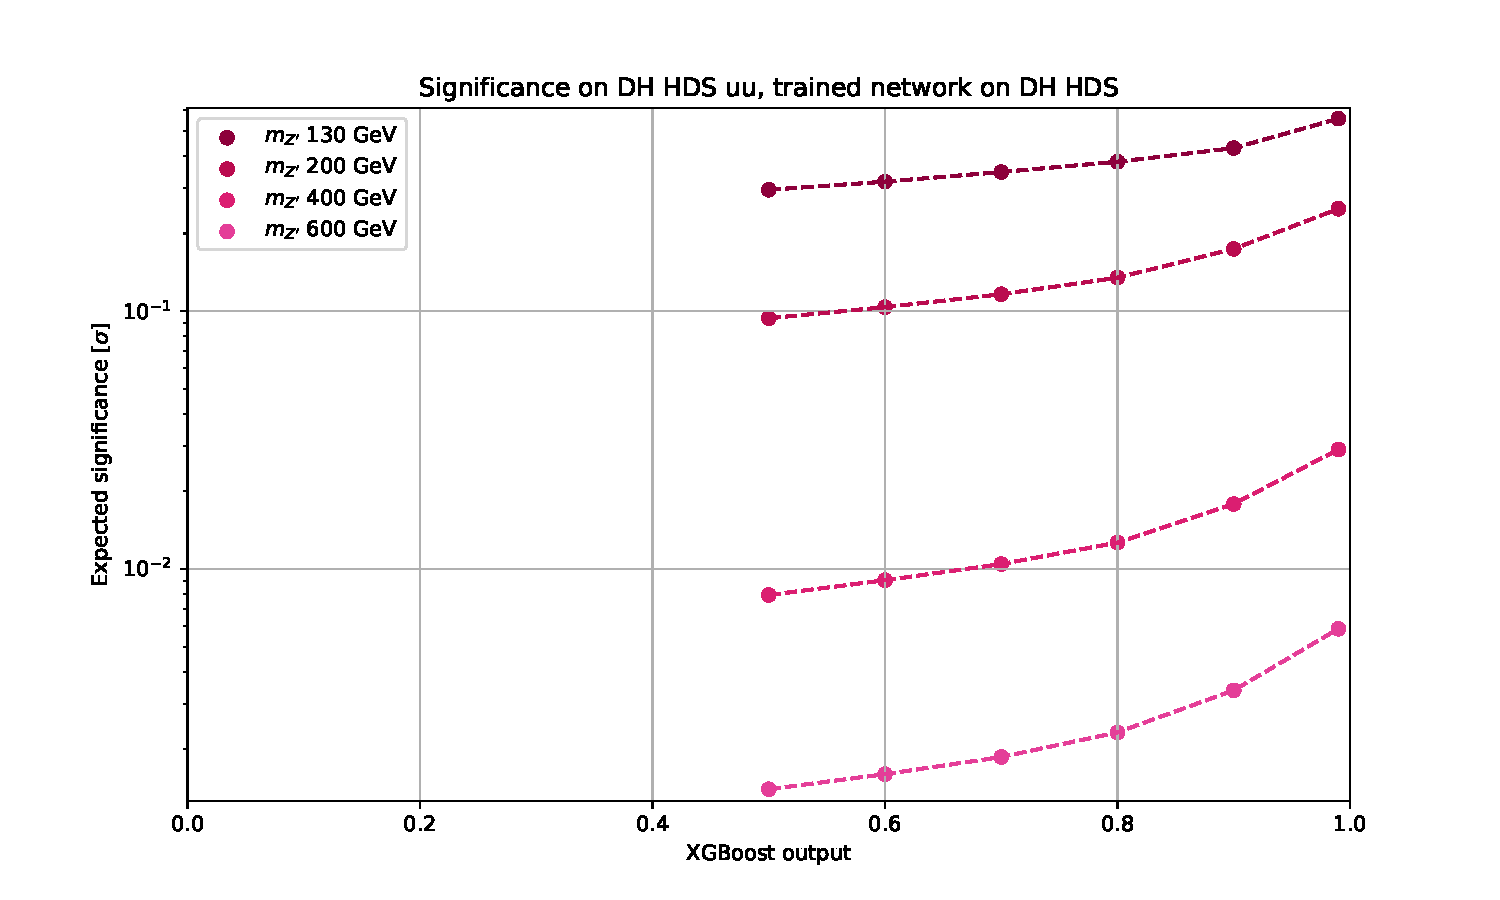
\includegraphics[width=1\textwidth]{XGBoost/DH_HDS/EXP_SIG_uu.pdf}
      \end{subfigure}
   \caption{Expected significance plots for Z' mass points on network trained on Z' DH HDS}\label{fig:DH_HDS_exp_sig}
\end{figure}
\\Using the last bin as the significance is greatest there, such that we effectively make a cut based on the BDT score. Using the last bin, we can calculate a mass exclusion for both electron and muon channel.\\
\\To do so we need to count the number of signal and background events that are on the last bin, as well as their uncertainties. Aditionally we will include the number of real data events that are there such that we can follow the 
method explained in Chapter \ref{sec:stat_anal}. In Table \ref{tab:stat_vals_DH_HDS} we see the values for each Z' mass point



\begin{table}[!ht]\centering\caption{Inputs for the $Z'h_D\rightarrow l^+l^-\chi\overline{\chi}$ $\sigma B$ calculations. The first three columns are the $Z'$ mass, the theoretical cross section times branching ratio $\sigma B$, and what $Z'$ decay channel we are looking at. 
   The next two are $\varepsilon_{\text{sig}}$, which is the signal selection efficiency, and $N_{\text{sig}}$, which is the theoretical number of signal events after the cuts. The last two columns are the number of background events, $N_{\text{bkg}}$, 
   and the events observed in the data, $N_{\text{obs}}$. The uncertainties of $\varepsilon_{\text{sig}}$, $N_{\text{sig}}$ and $N_{\text{bkg}}$ are statistical with an assumed 20\% systematic uncertainty. The MET threshold is $E_{\text{T,min}}^{\text{miss}}=110$GeV 
   and is the same for all inputs.}
   \begin{tabular}{@{}ccc|cccc@{}}
   \midrule\midrule
   $m_{Z'}$ [GeV] & $\sigma B$ [fb] & Channel & $\varepsilon_{\text{sig}}$& $N_{\text{sig}}$ & $N_{\text{bkg}}$ & $N_{\text{obs}}$\\\midrule\midrule
   \multirow{2}{*}[-2\baselineskip]{130}& \multirow{2}{*}[-2\baselineskip]{1.110220011923957}& $e^+e^-$ & $0.02526\pm0.0107$ & $1329\pm318$ & $334.8\pm14.6$ & 452\\
   & & $\mu^+\mu^-$ & $0.02033\pm8.85$ & $1107\pm307$ & $326.1\pm17.2$ & 382\\\midrule
   \multirow{2}{*}[-2\baselineskip]{200}& \multirow{2}{*}[-2\baselineskip]{0.24630000439174182}& $e^+e^-$ & $0.05361\pm0.0225$ & $91.4\pm21.7$ & $334.8\pm14.6$ & 452\\
   & & $\mu^+\mu^-$ & $49.9\pm12.7$ & $89.4\pm22.2$ & $326.1\pm17.2$ & 382\\\midrule
   \multirow{2}{*}[-2\baselineskip]{400}& \multirow{2}{*}[-2\baselineskip]{0.01489120027287072}& $e^+e^-$ & $0.11273\pm0.0279$ & $34.1\pm8.15\pm \beta$ & $334.8\pm14.6$ & 452\\
   & & $\mu^+\mu^-$ & $54.0\pm12.7$ & $32.7\pm7.65$ & $326.1\pm17.2$ & 382\\\midrule
   \multirow{2}{*}[-2\baselineskip]{600}& \multirow{2}{*}[-2\baselineskip]{0.0023450000830038675}& $e^+e^-$ & $0.13996\pm0.0317$ & $17.1\pm3.88$ & $334.8\pm14.6$ & 452\\
   & & $\mu^+\mu^-$ & $49.4\pm13.1$ & $14.6\pm3.79$ & $326.1\pm17.2$ & 382\\\midrule
   \multirow{2}{*}[-2\baselineskip]{800}& \multirow{2}{*}[-2\baselineskip]{0.0005433999916704124}& $e^+e^-$ & $0.15894\pm0.0319$ & $9.72\pm2.24$ & $334.8\pm14.6$ & 452\\
   & & $\mu^+\mu^-$ & $49.3\pm13.7$ & $7.42\pm2.03$ & $326.1\pm17.2$ & 382\\\midrule
   \multirow{2}{*}[-2\baselineskip]{900}& \multirow{2}{*}[-2\baselineskip]{0.00028203001045667975}& $e^+e^-$ & $0.15990\pm0.0326$ & $5.24\pm1.32$ & $334.8\pm14.6$ & 452\\
   & & $\mu^+\mu^-$ & $51.0\pm13.6$ & $4.54\pm1.19$ & $326.1\pm17.2$ & 382\\\midrule
   \multirow{2}{*}[-2\baselineskip]{1100}& \multirow{2}{*}[-2\baselineskip]{8.400600007285597e-05}& $e^+e^-$ & $0.16309\pm0.0330$ & $3.074\pm0.789$ & $334.8\pm14.6$ & 452\\
   & & $\mu^+\mu^-$ & $49.0\pm13.3$ & $2.868\pm0.759$ & $326.1\pm17.2$ & 382\\\midrule
   \multirow{2}{*}[-2\baselineskip]{1200}& \multirow{2}{*}[-2\baselineskip]{4.745799933592032e-05}& $e^+e^-$ & $0.16510\pm0.0337$ & $2.254\pm0.569$ & $334.8\pm14.6$ & 452\\
   & & $\mu^+\mu^-$ & $48.2\pm13.0$ & $1.885\pm0.499$ & $326.1\pm17.2$ & 382\\\midrule
   \multirow{2}{*}[-2\baselineskip]{1300}& \multirow{2}{*}[-2\baselineskip]{2.731299995201164e-05}& $e^+e^-$ & $0.16898\pm$ & $1.411\pm0.366$ & $334.8\pm14.6$ & 452\\
   & & $\mu^+\mu^-$ & $53.7\pm14.1$ & $1.436\pm0.369$ & $326.1\pm17.2$ & 382\\\midrule
   \multirow{2}{*}[-2\baselineskip]{1400}& \multirow{2}{*}[-2\baselineskip]{1.596690054478378e-05}& $e^+e^-$ & $0.16728\pm$ & $0.0411\pm0.0112$ & $334.8\pm14.6$ & 452\\
   & & $\mu^+\mu^-$ & $39.0\pm11.1$ & $0.0387\pm0.0108$ & $326.1\pm17.2$ & 382\\
   \multirow{2}{*}[-2\baselineskip]{1500}& \multirow{2}{*}[-2\baselineskip]{9.424799916196713e-06}& $e^+e^-$ & $0.16938\pm$ & $0.0411\pm0.0112$ & $334.8\pm14.6$ & 452\\
   & & $\mu^+\mu^-$ & $39.0\pm11.1$ & $0.0387\pm0.0108$ & $326.1\pm17.2$ & 382\\\midrule\midrule
   \end{tabular}
   \label{tab:stat_vals_DH_HDS}
\end{table} 
\begin{figure}[!ht]
	\centering
   \begin{subfigure}[b]{0.49\textwidth}
      \centering
      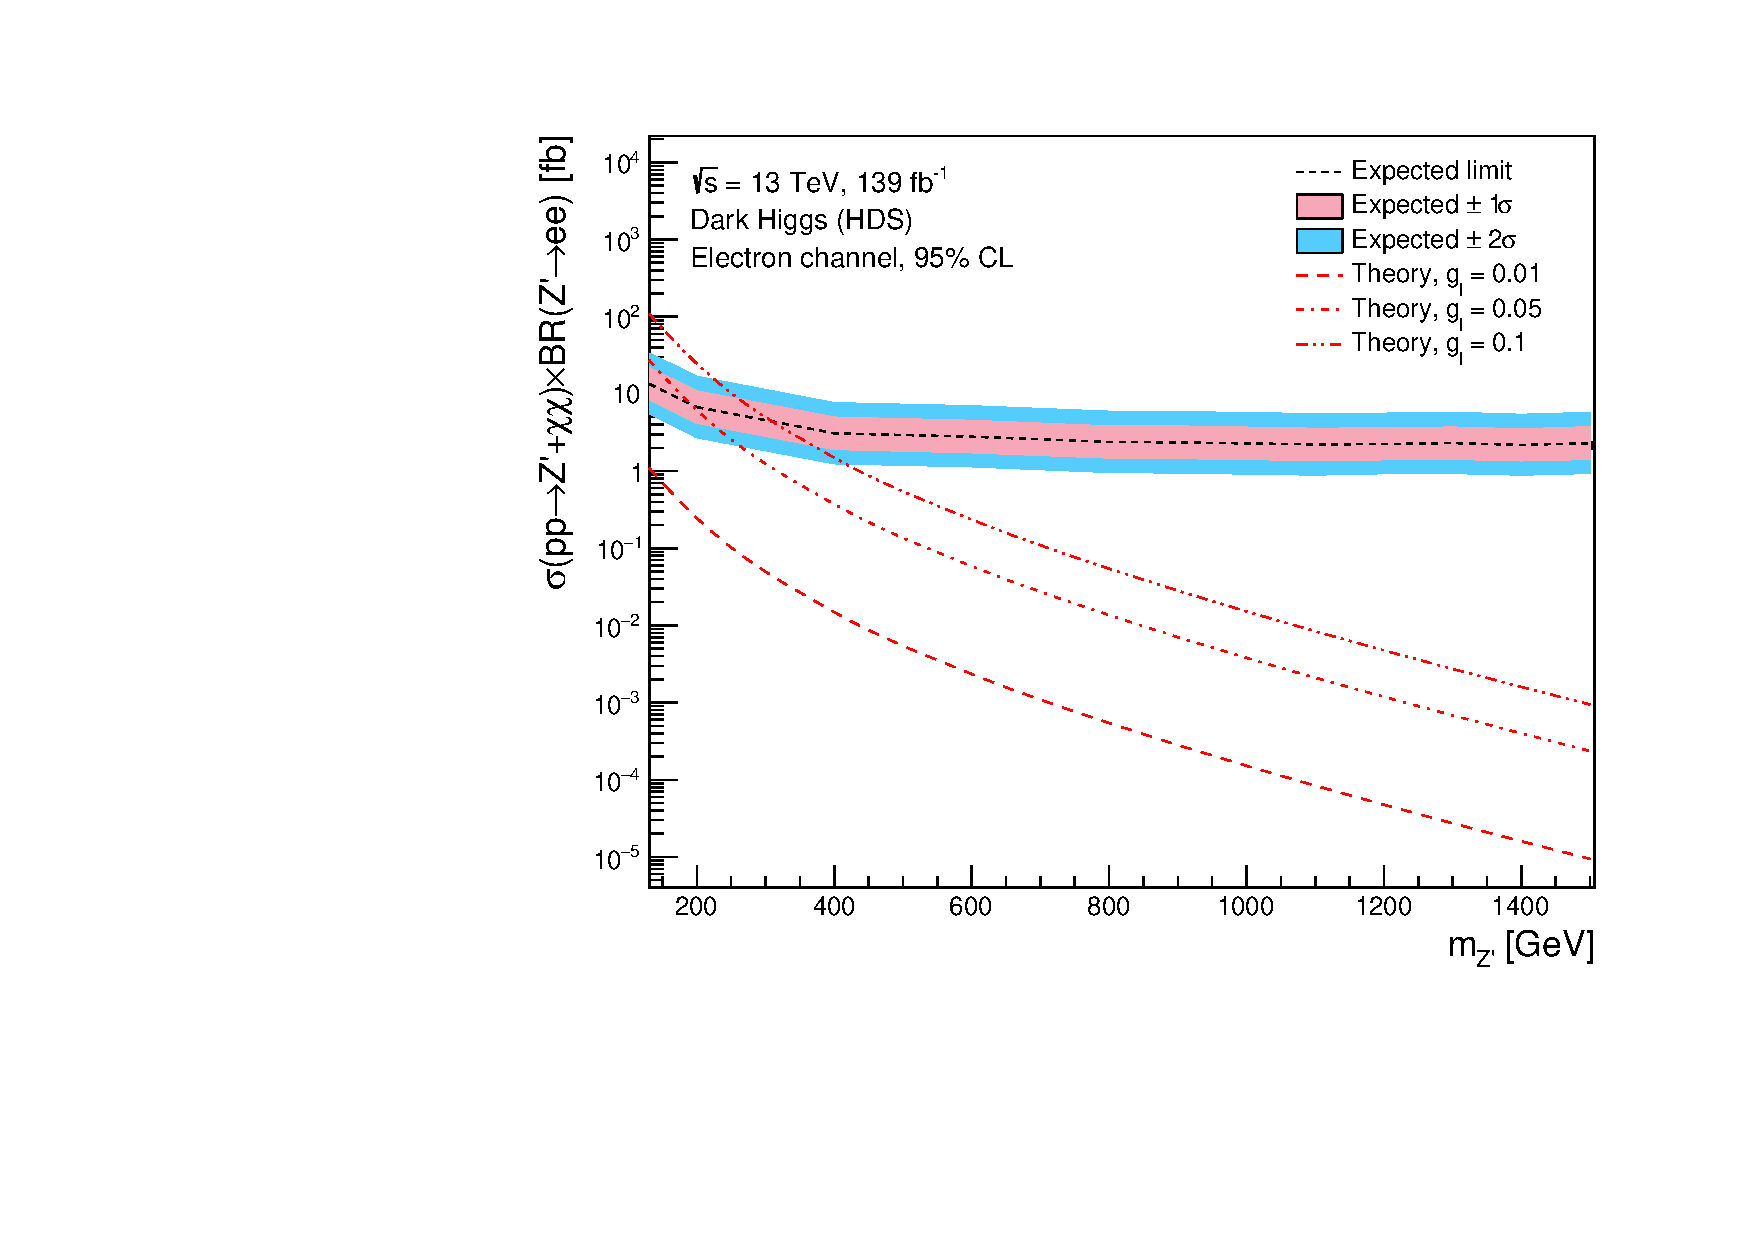
\includegraphics[width=1\textwidth]{Limits/DH_HDS/mass_exclusion_ee.pdf}
      \end{subfigure}
   \hfill
   \begin{subfigure}[b]{0.49\textwidth}
      \centering
      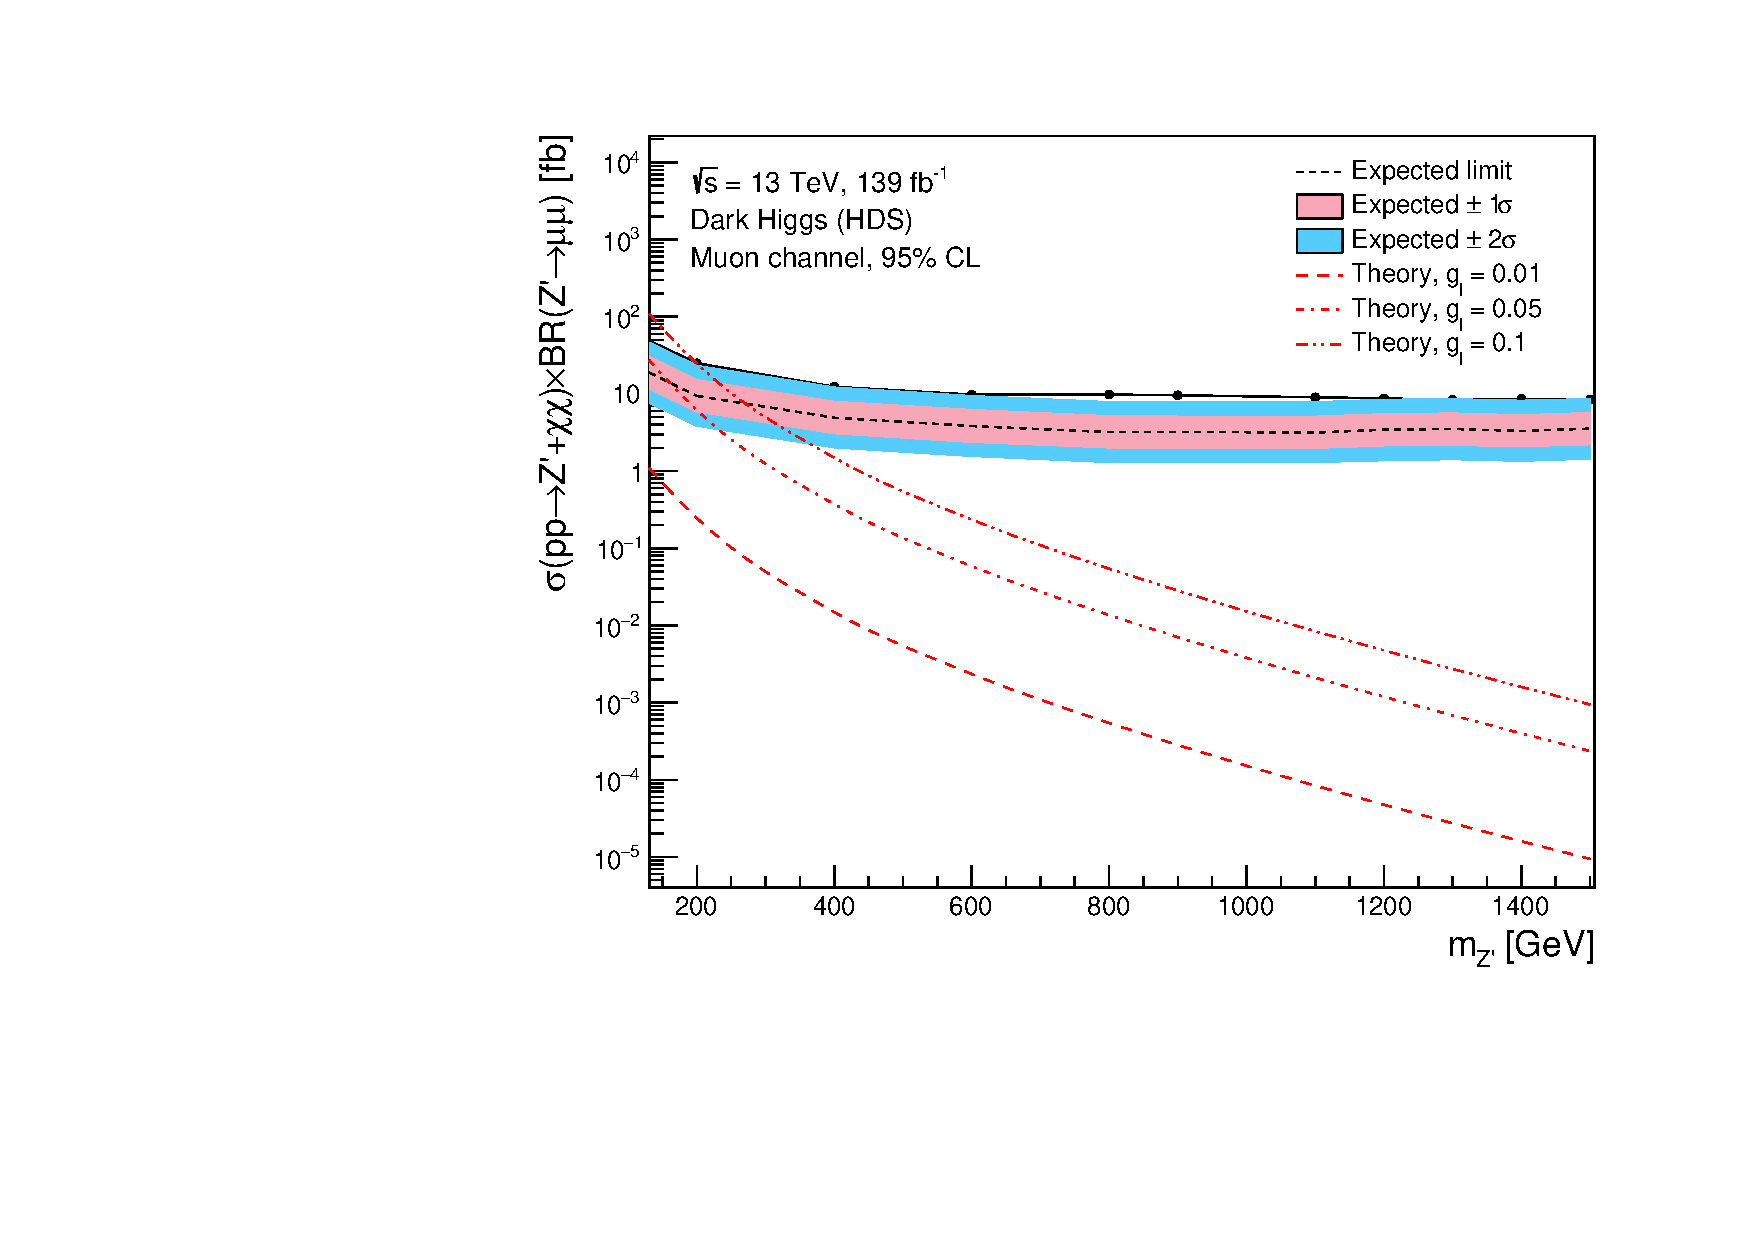
\includegraphics[width=1\textwidth]{Limits/DH_HDS/mass_exclusion_uu.pdf}
      \end{subfigure}
   \caption{Mass exclusion limits of $ee$ and $\mu\mu$ channel for all Z' DH HDS model}\label{fig:DH_HDS_exclusion_ee_uu}
\end{figure}
As the lepton coupling was chosen to be $g_l=0.001$ when simulating the data, by the assumption that the number of events that survived the cuts is the same, we can increase this coupling to see how the mass limits changes.

\newpage
\section{Dark Higgs Light Dark Sector}
Trained a network using all of the SM background samples and every different Z' mass of this model. Here are the results
\begin{figure}[!ht]
	\centering
	\begin{subfigure}[b]{0.49\textwidth}
      \centering
      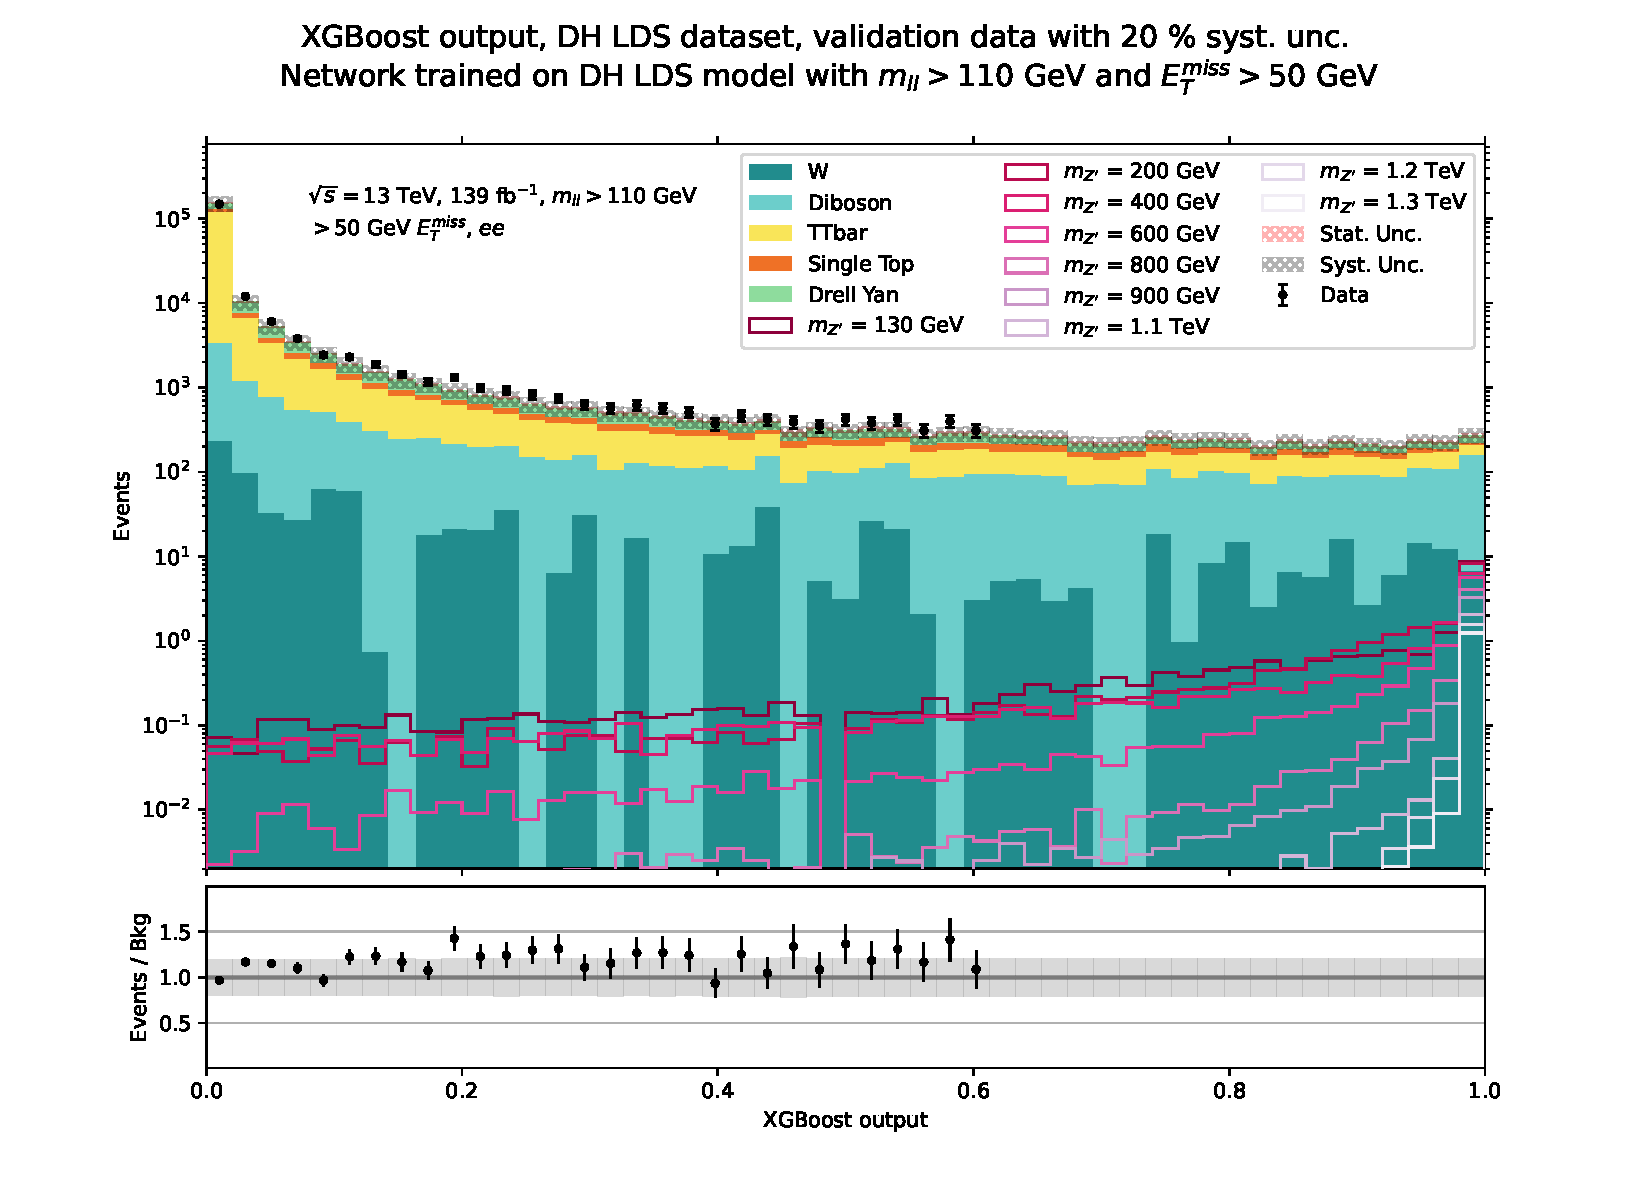
\includegraphics[width=1\textwidth]{XGBoost/DH_LDS/VAL_ee.pdf}
      \end{subfigure}
   \hfill
   \begin{subfigure}[b]{0.49\textwidth}
      \centering
      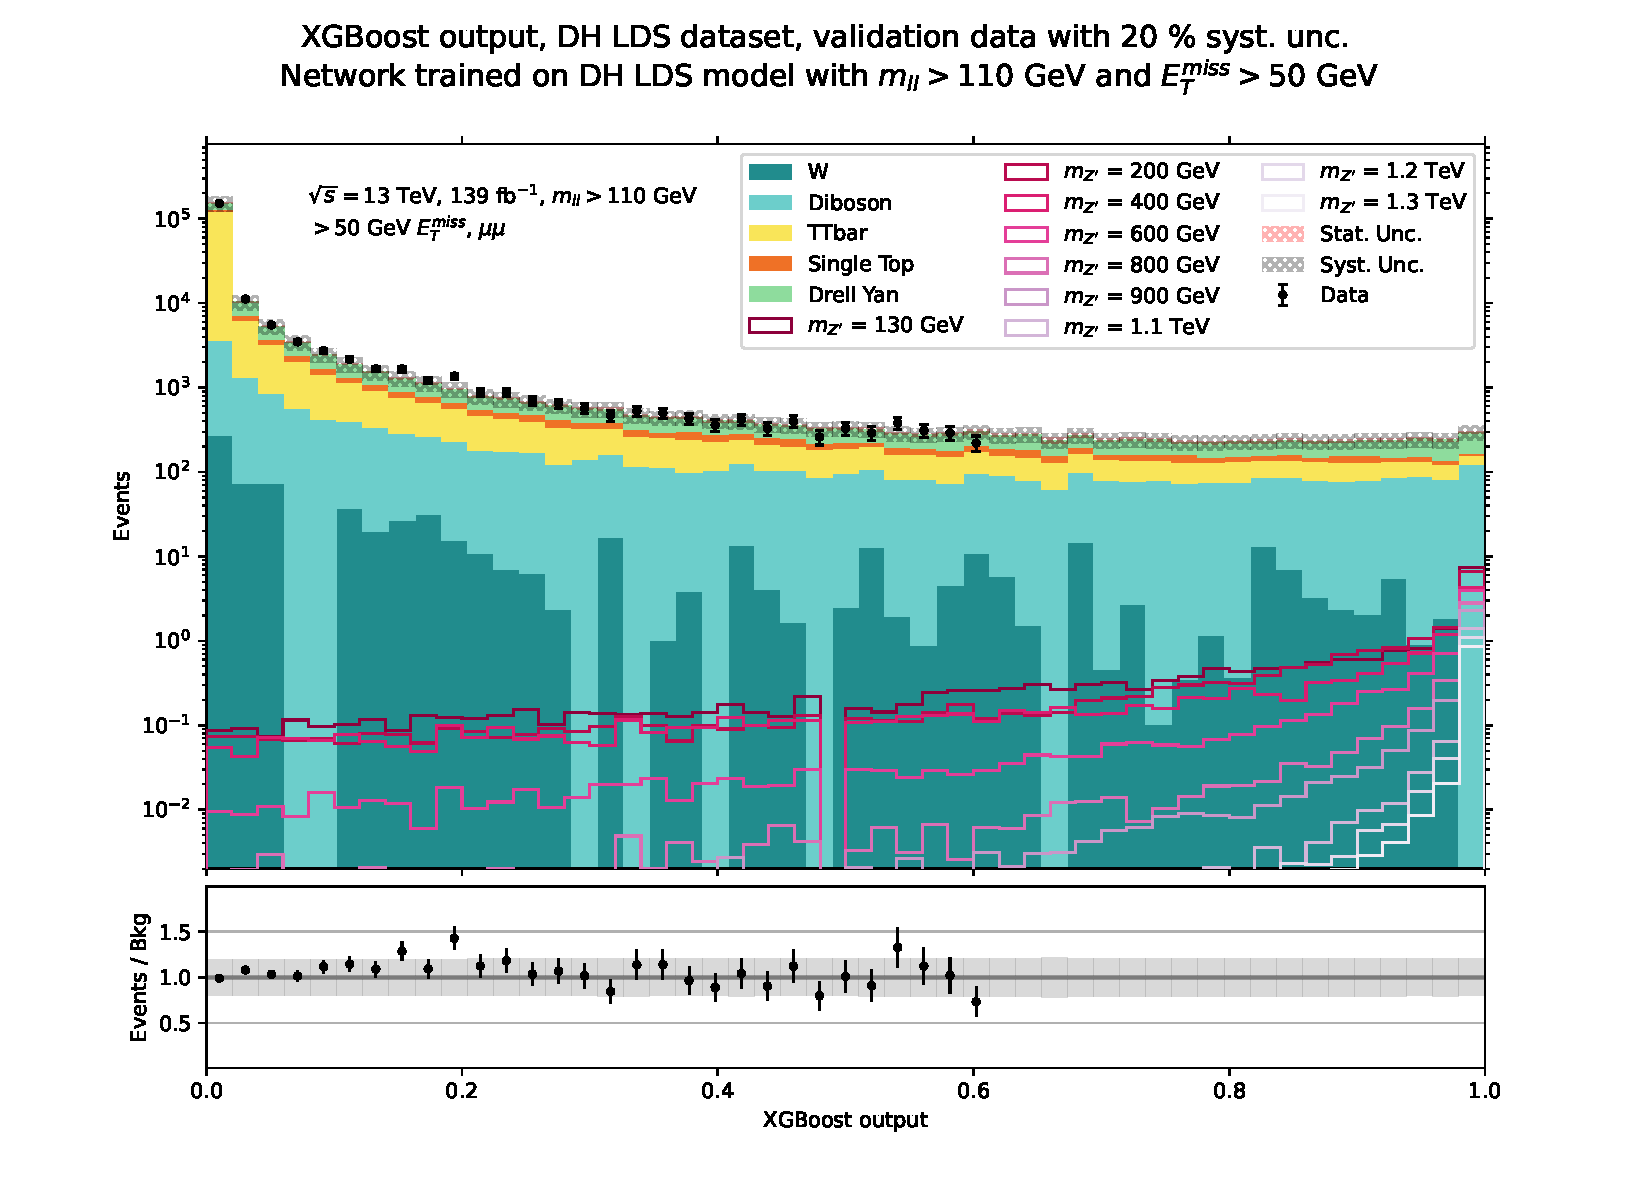
\includegraphics[width=1\textwidth]{XGBoost/DH_LDS/VAL_uu.pdf}
      \end{subfigure}
   \caption{Validation plots for network trained on Z' DH LDS}\label{fig:DH_LDS_vals}
\end{figure}
\\With the ROC for each mass point seen in Figure \ref{fig:DH_LDS_ROCS}.
\begin{figure}[!ht]
	\centering
	\begin{subfigure}[b]{0.49\textwidth}
      \centering
      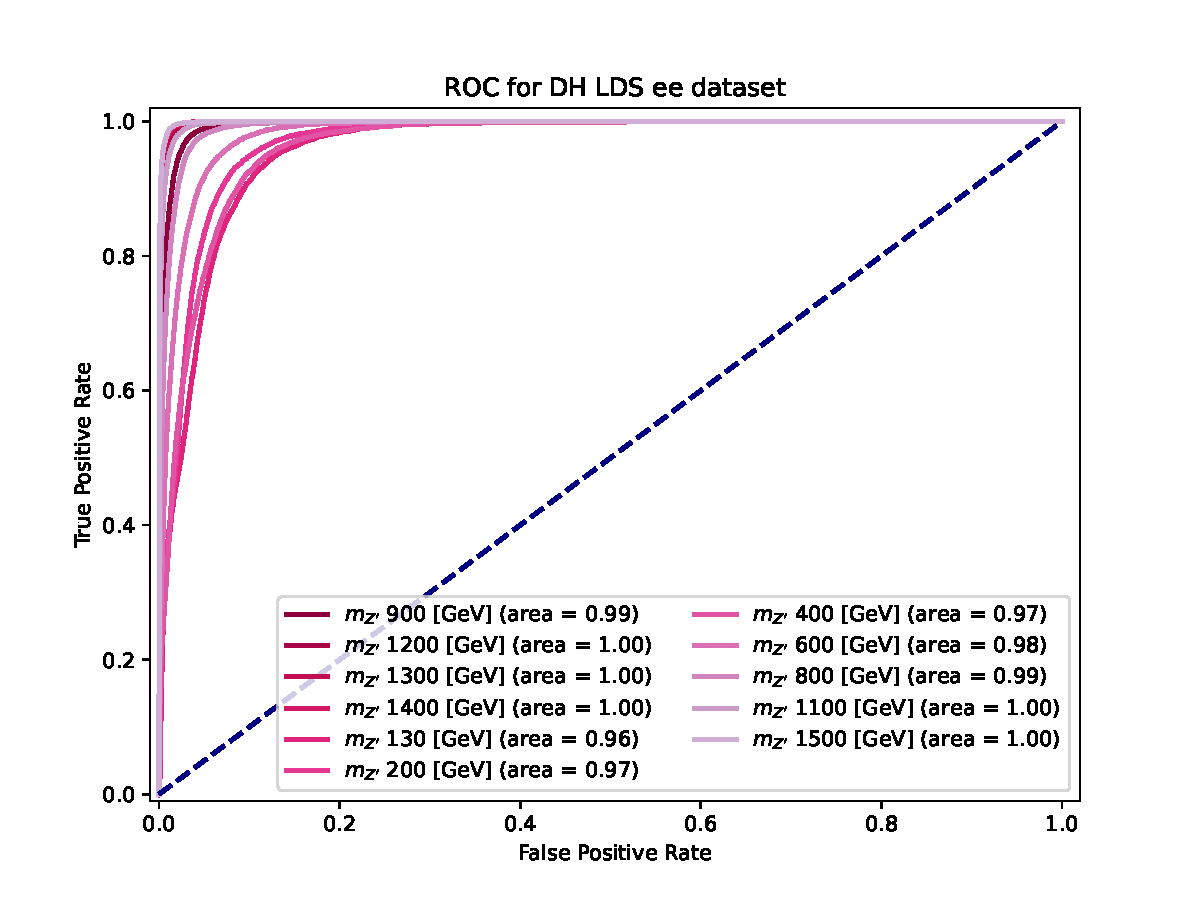
\includegraphics[width=1\textwidth]{XGBoost/DH_LDS/ROC_ee.pdf}
      \end{subfigure}
   \hfill
   \begin{subfigure}[b]{0.49\textwidth}
      \centering
      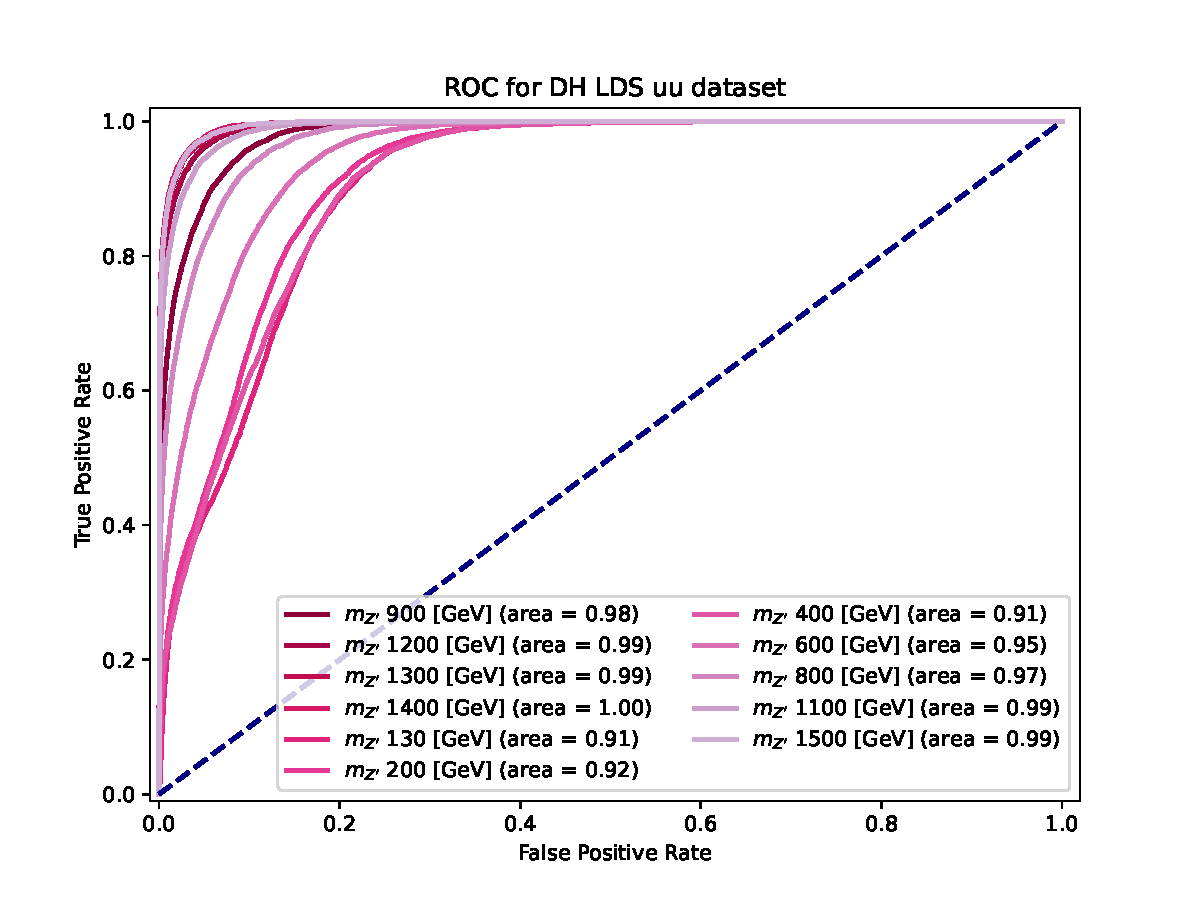
\includegraphics[width=1\textwidth]{XGBoost/DH_LDS/ROC_uu.pdf}
      \end{subfigure}
   \caption{ROC plots for every Z' mass point on network trained on Z' DH LDS}\label{fig:DH_LDS_ROCS}
\end{figure}
\\Plotting the significance of the models given the binning we get the results from Figure \ref{fig:DH_LDS_exp_sig}
\begin{figure}[!ht]
	\centering
	\begin{subfigure}[b]{0.49\textwidth}
      \centering
      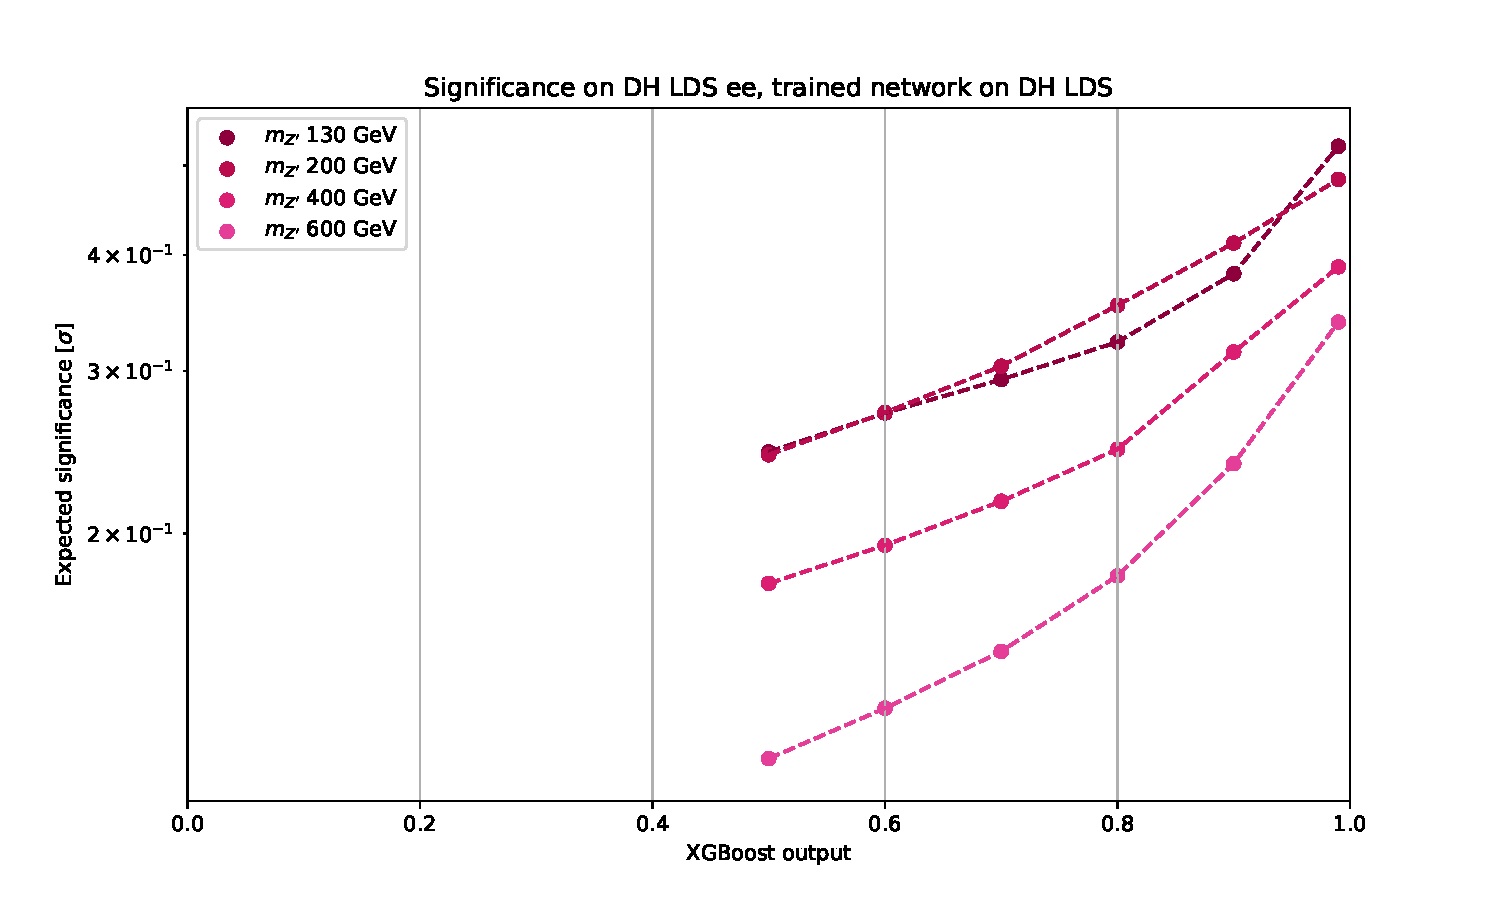
\includegraphics[width=1\textwidth]{XGBoost/DH_LDS/EXP_SIG_ee.pdf}
      \end{subfigure}
   \hfill
   \begin{subfigure}[b]{0.49\textwidth}
      \centering
      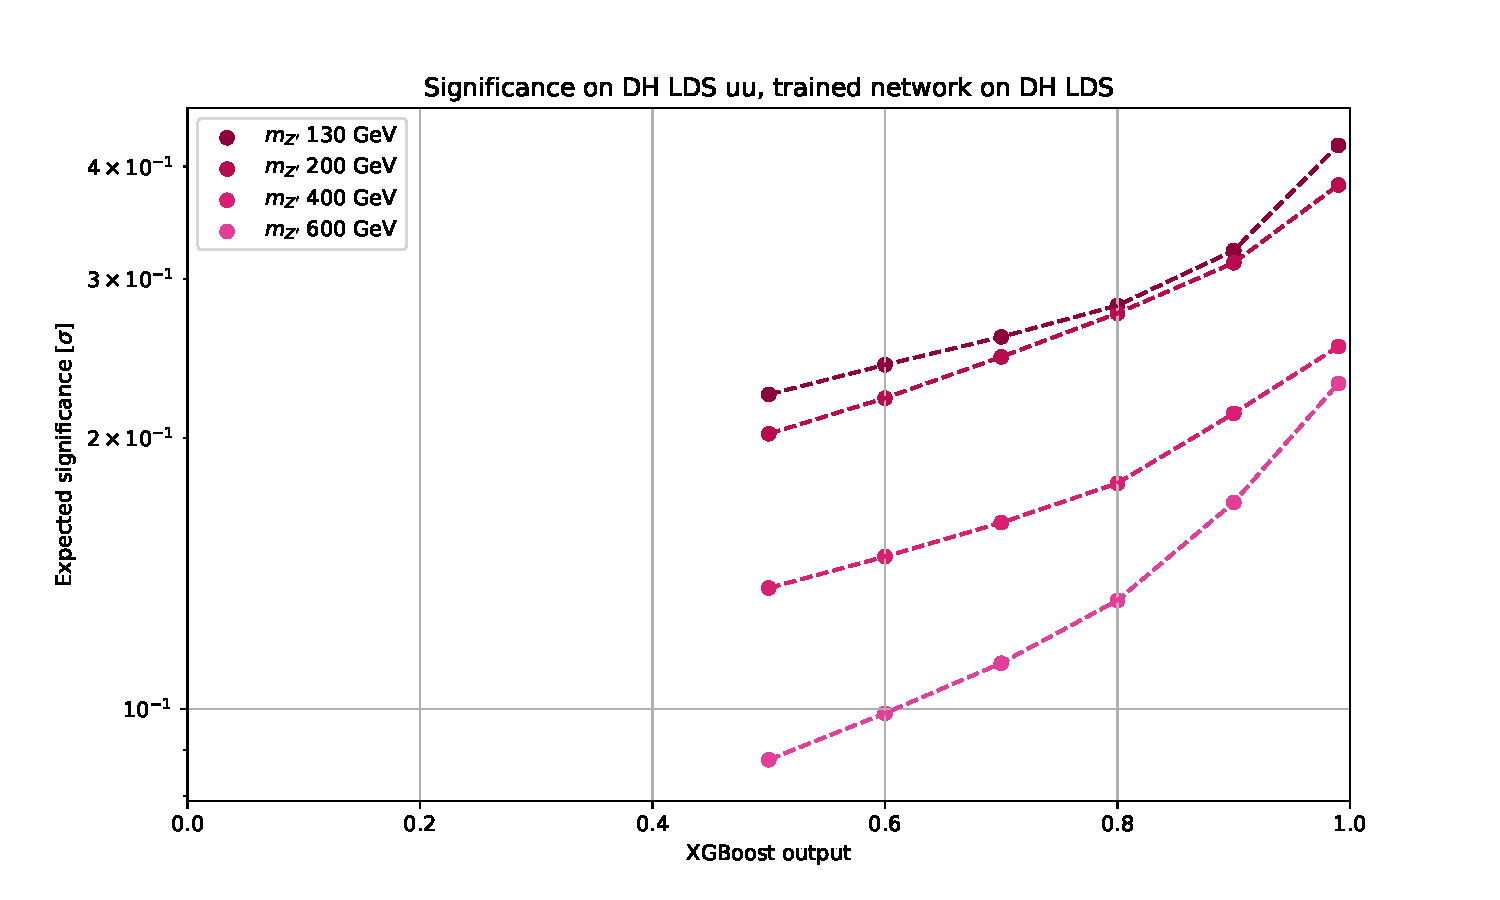
\includegraphics[width=1\textwidth]{XGBoost/DH_LDS/EXP_SIG_uu.pdf}
      \end{subfigure}
   \caption{Expected significance plots for Z' mass points on network trained on Z' DH LDS}\label{fig:DH_LDS_exp_sig}
\end{figure}
\\Using the last bin as the significance is greatest there, such that we effectively make a cut based on the BDT score. Using the last bin, we can calculate a mass exclusion for both electron and muon channel.\\
\\To do so we need to count the number of signal and background events that are on the last bin, as well as their uncertainties. Aditionally we will include the number of real data events that are there such that we can follow the 
method explained in Chapter \ref{sec:stat_anal}. In Table \ref{tab:stat_vals_DH_LDS} we see the values for each Z' mass point.
\begin{figure}[!ht]
	\centering
   \begin{subfigure}[b]{0.49\textwidth}
      \centering
      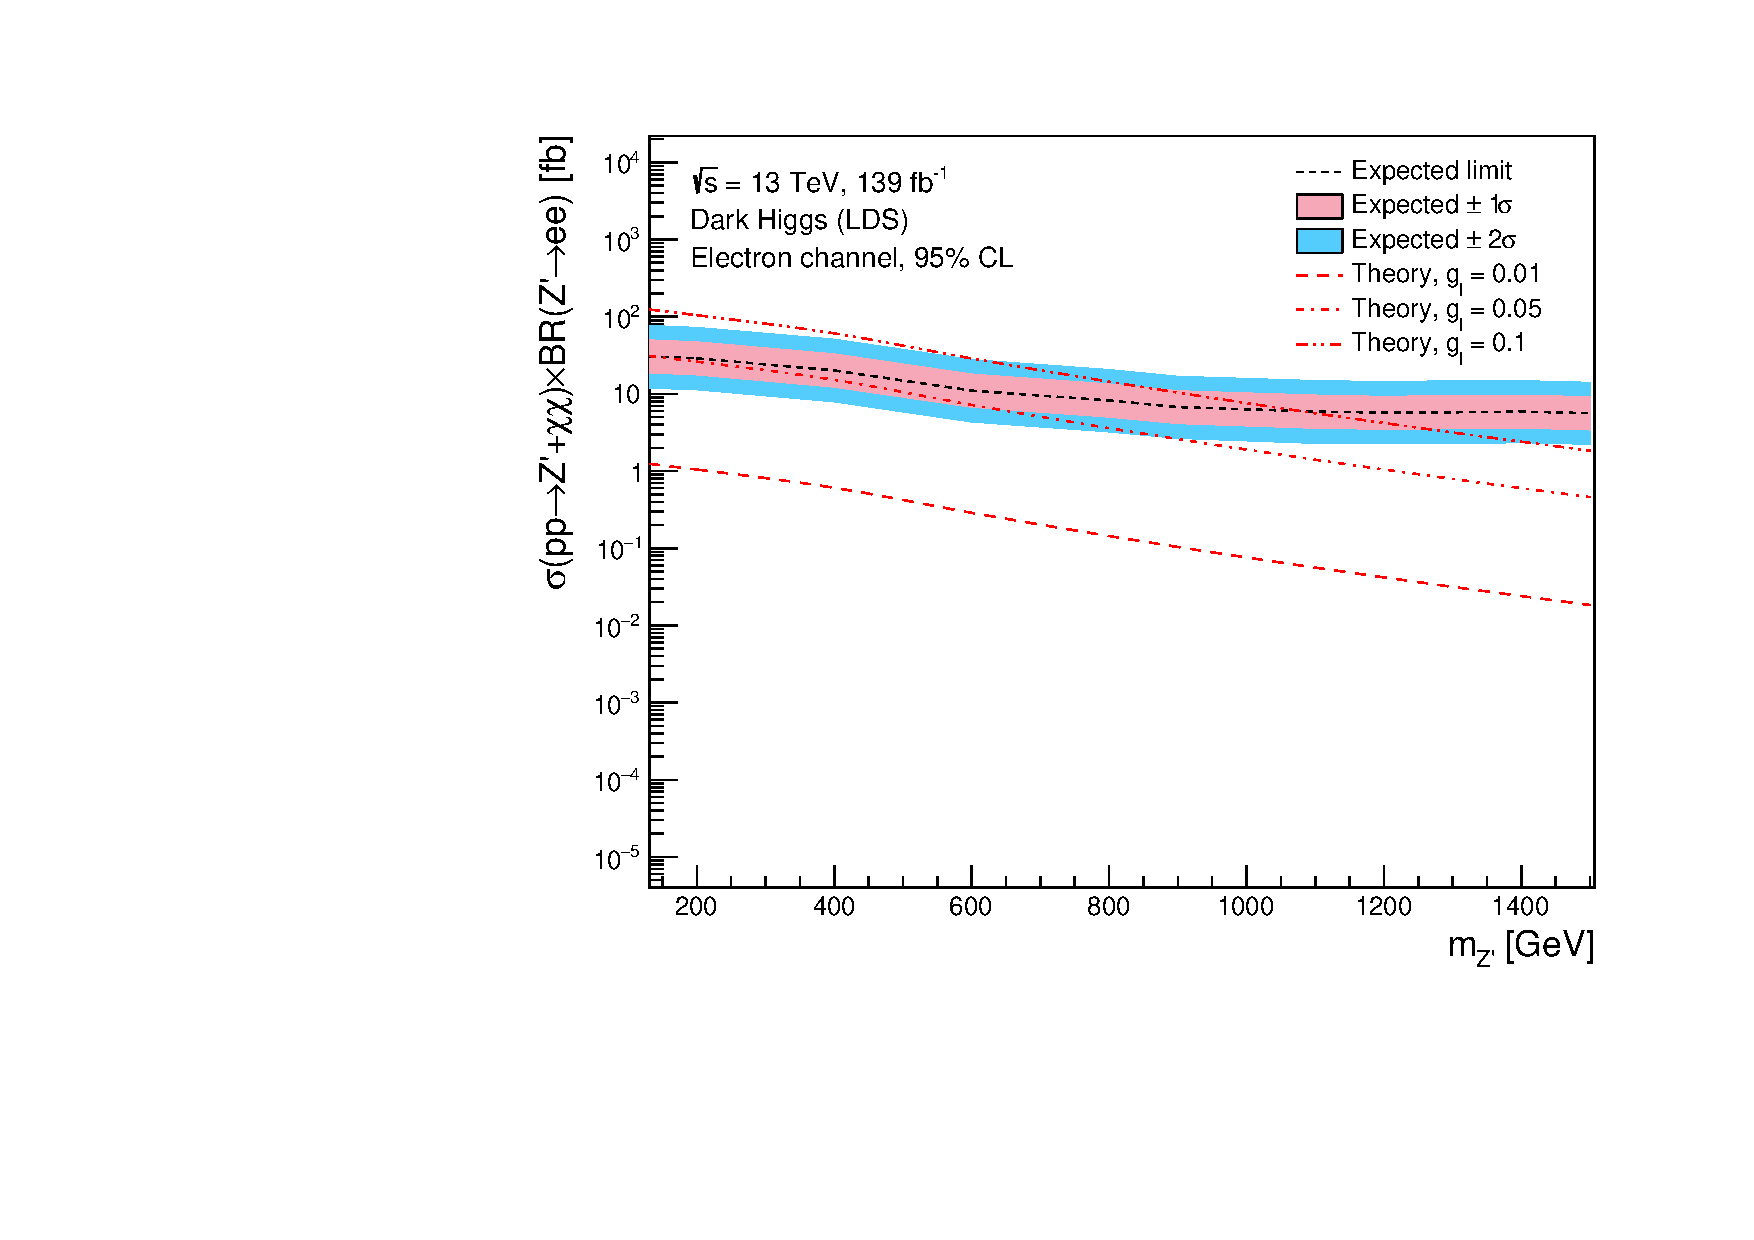
\includegraphics[width=1\textwidth]{Limits/DH_LDS/mass_exclusion_ee.pdf}
      \end{subfigure}
   \hfill
   \begin{subfigure}[b]{0.49\textwidth}
      \centering
      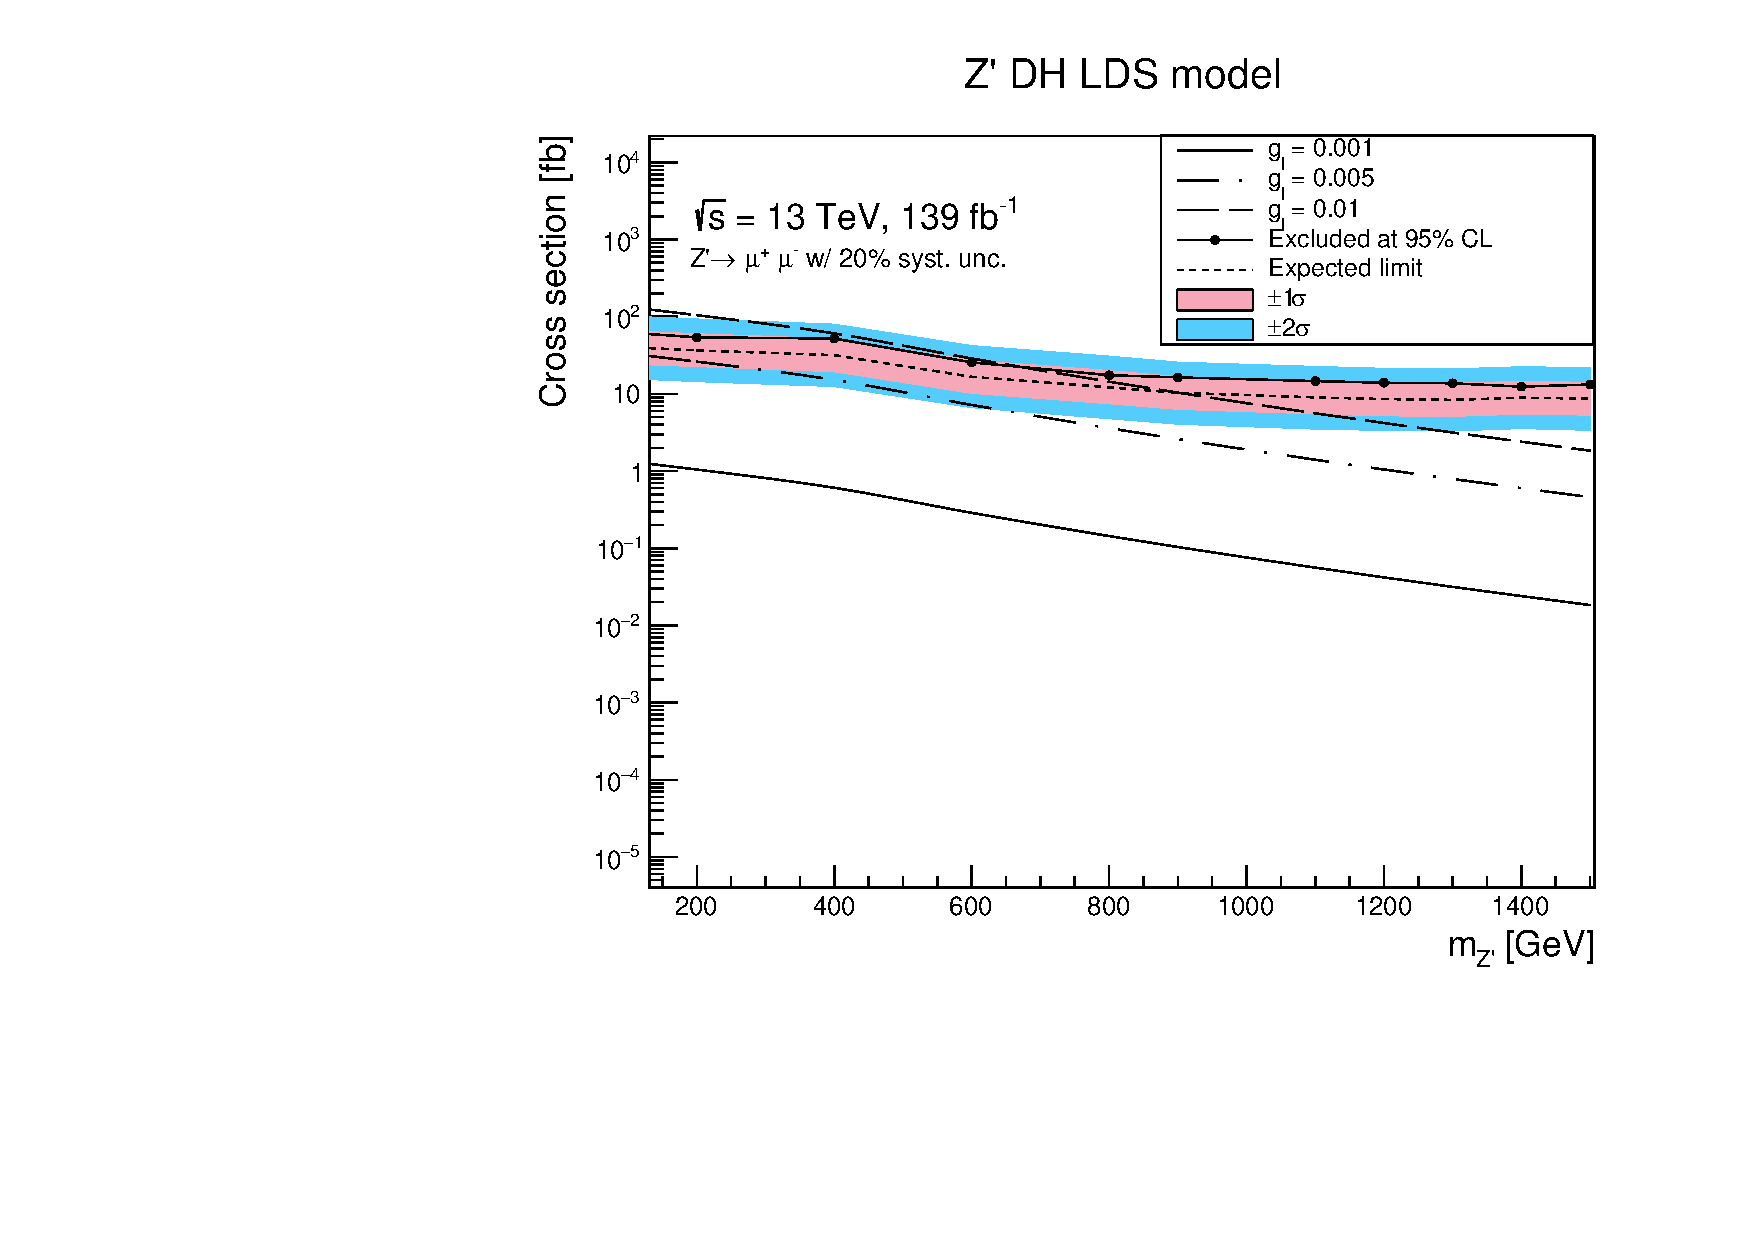
\includegraphics[width=1\textwidth]{Limits/DH_LDS/mass_exclusion_uu.pdf}
      \end{subfigure}
   \caption{Mass exclusion limits of $ee$ and $\mu\mu$ channel for all Z' DH LDS model}\label{fig:DH_LDS_exclusion_ee_uu}
\end{figure}
As the lepton coupling was chosen to be $g_l=0.001$ when simulating the data, by the assumption that the number of events that survived the cuts is the same, we can increase this coupling to see how the mass limits changes.


\newpage
\section{Light Vector Heavy Dark Sector}
Trained a network using all of the SM background samples and every different Z' mass of this model. Here are the results
\begin{figure}[!ht]
	\centering
	\begin{subfigure}[b]{0.49\textwidth}
      \centering
      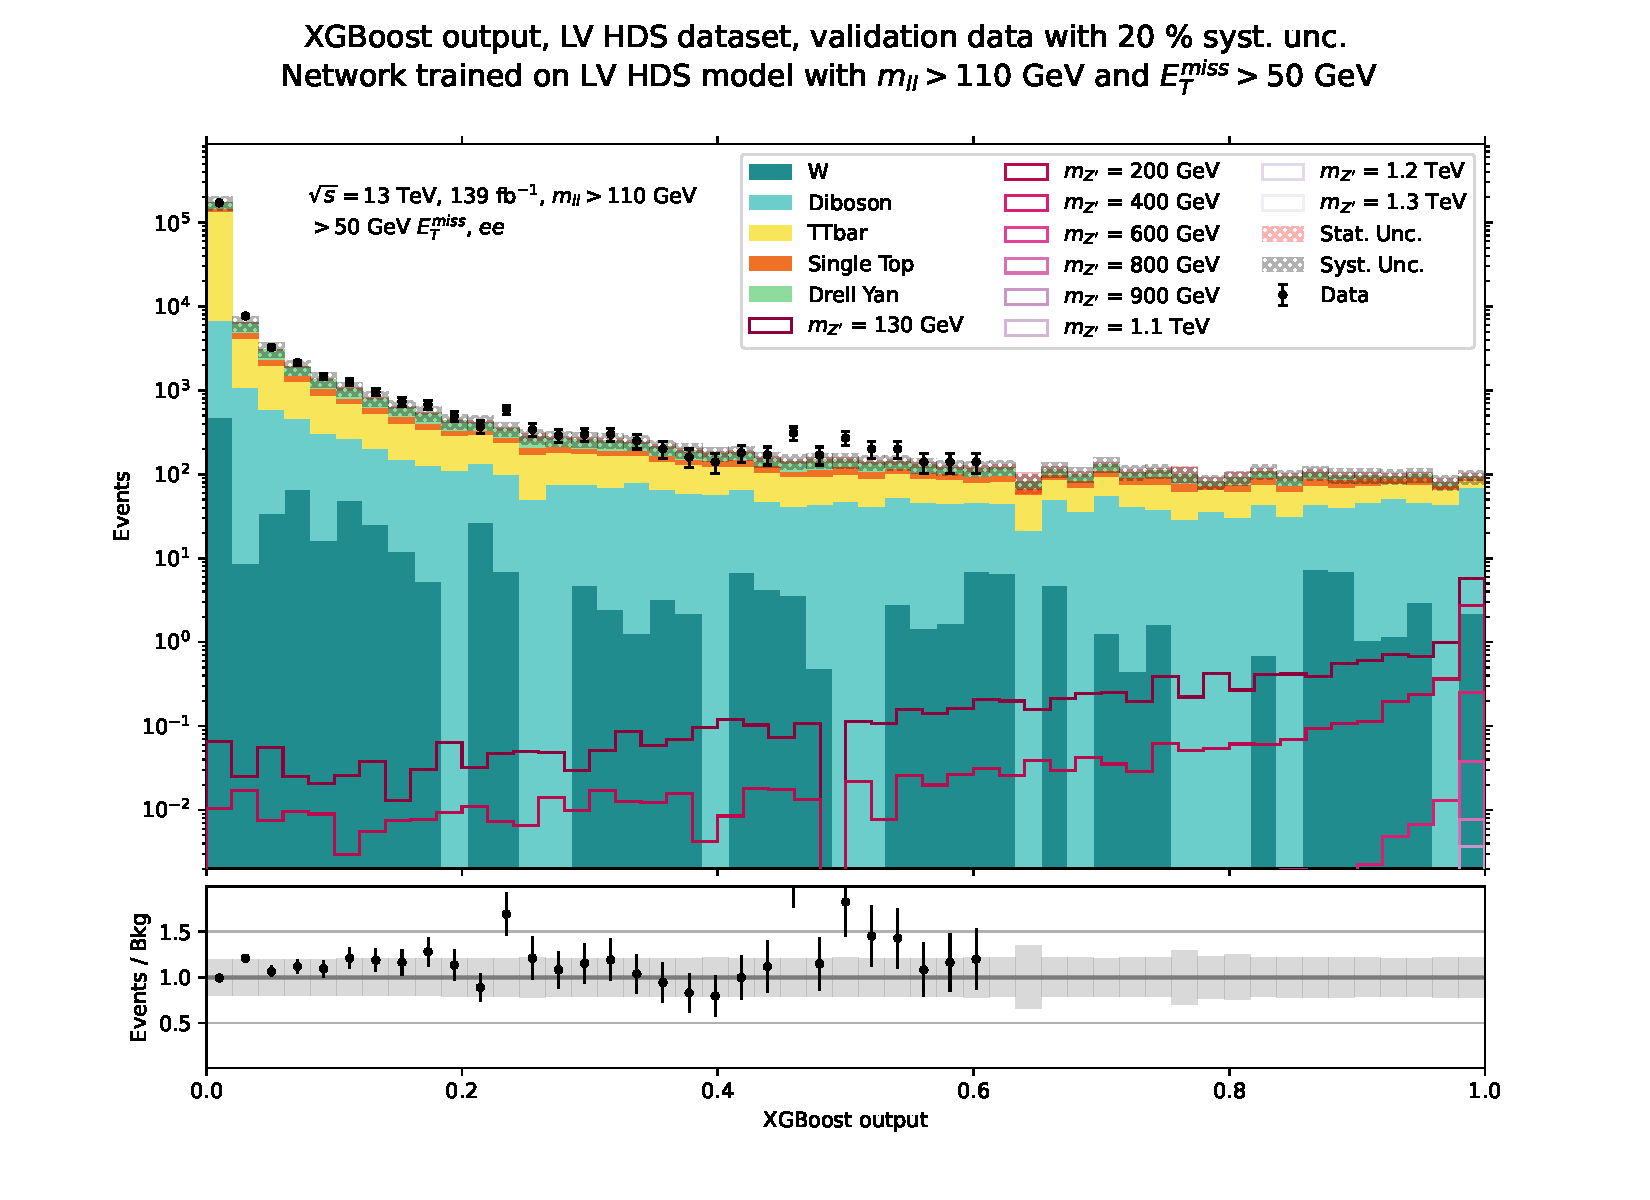
\includegraphics[width=1\textwidth]{XGBoost/LV_HDS/VAL_ee.pdf}
      \end{subfigure}
   \hfill
   \begin{subfigure}[b]{0.49\textwidth}
      \centering
      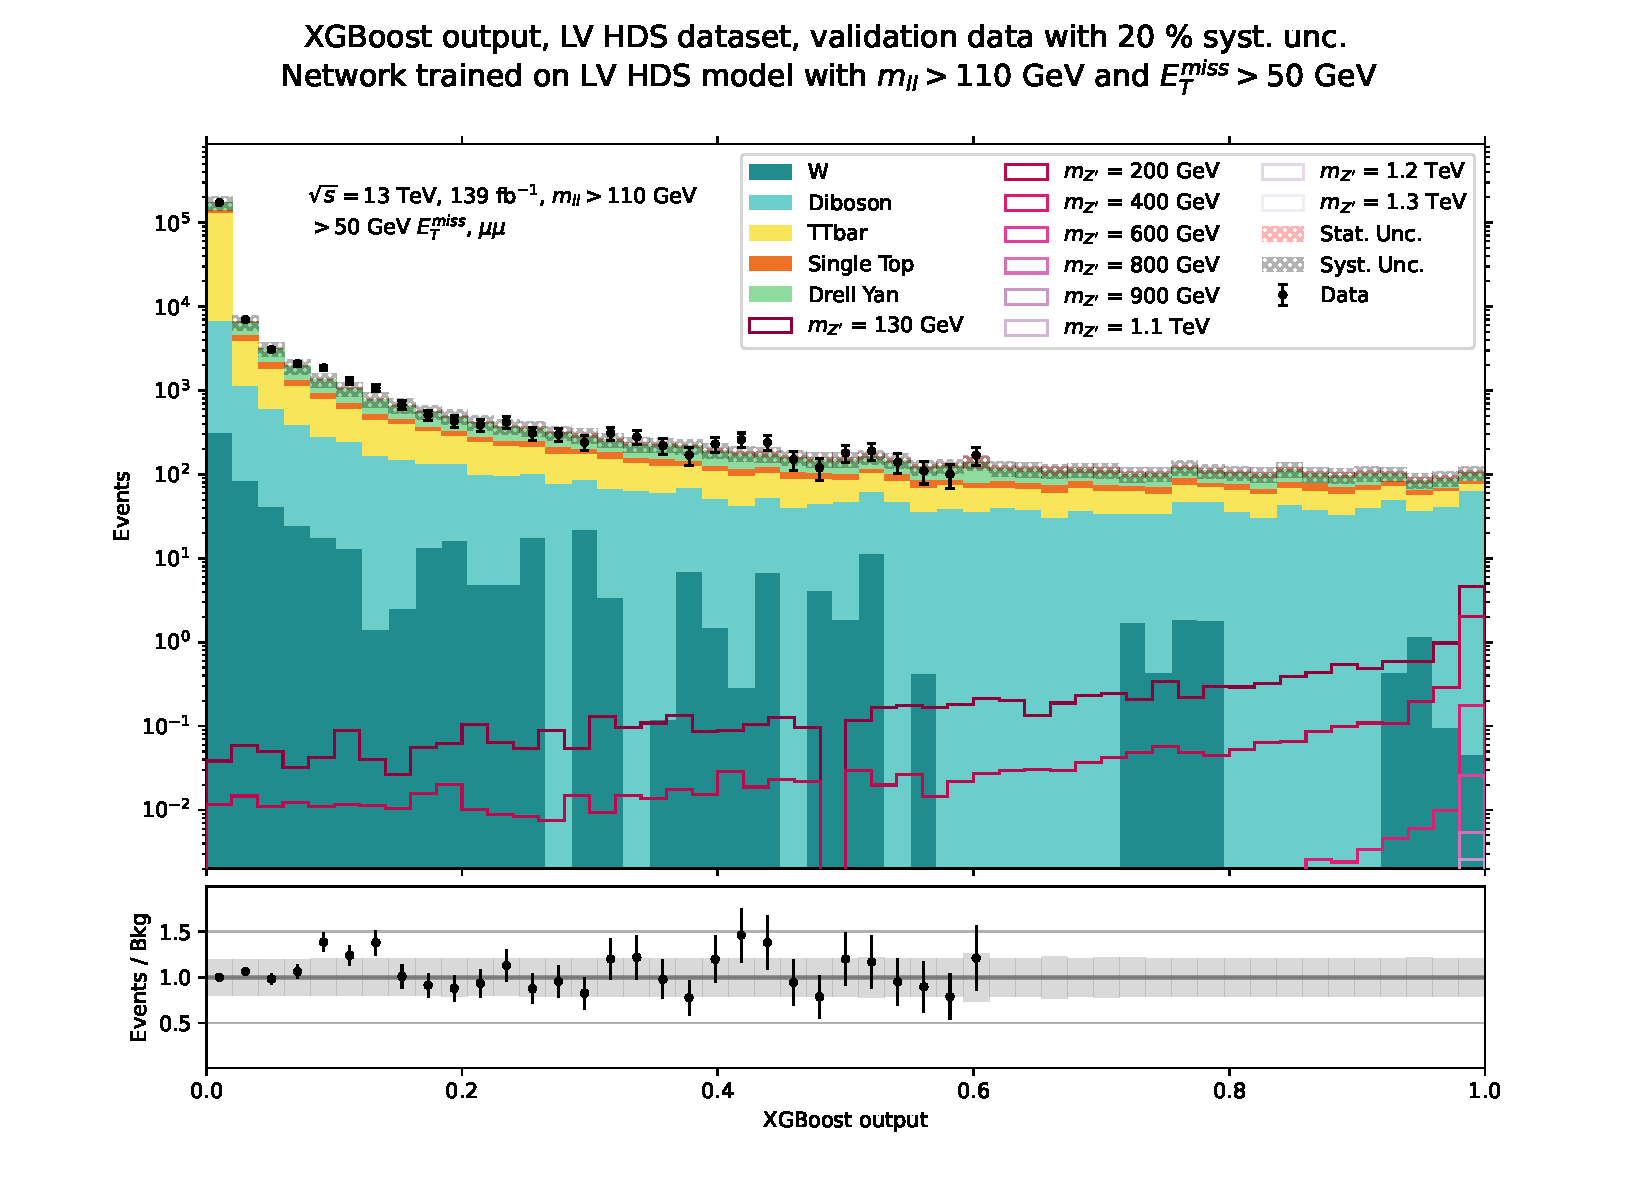
\includegraphics[width=1\textwidth]{XGBoost/LV_HDS/VAL_uu.pdf}
      \end{subfigure}
   \caption{Validation plots for network trained on Z' LV HDS}\label{fig:LV_HDS_vals}
\end{figure}
\\With the ROC for each mass point seen in Figure \ref{fig:LV_HDS_ROCS}.
\begin{figure}[!ht]
	\centering
	\begin{subfigure}[b]{0.49\textwidth}
      \centering
      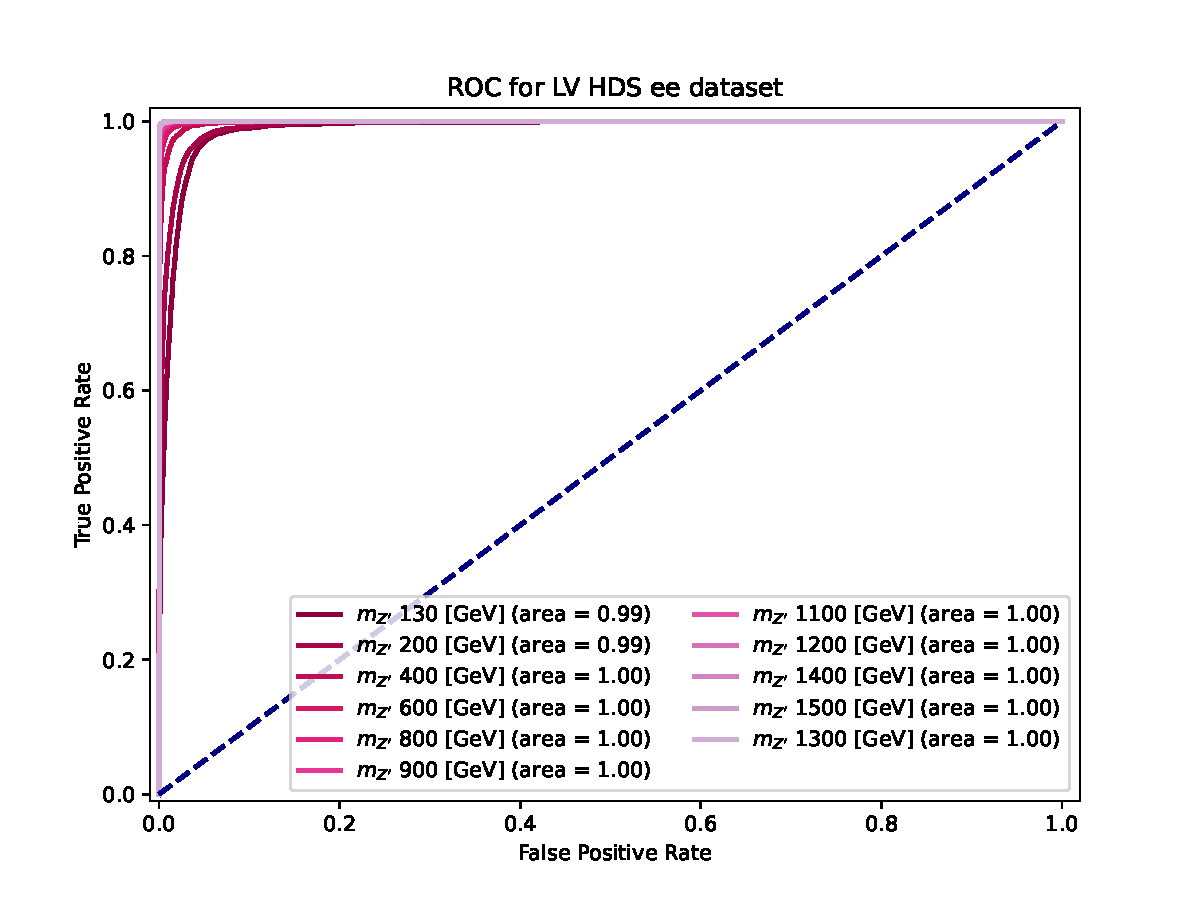
\includegraphics[width=1\textwidth]{XGBoost/LV_HDS/ROC_ee.pdf}
      \end{subfigure}
   \hfill
   \begin{subfigure}[b]{0.49\textwidth}
      \centering
      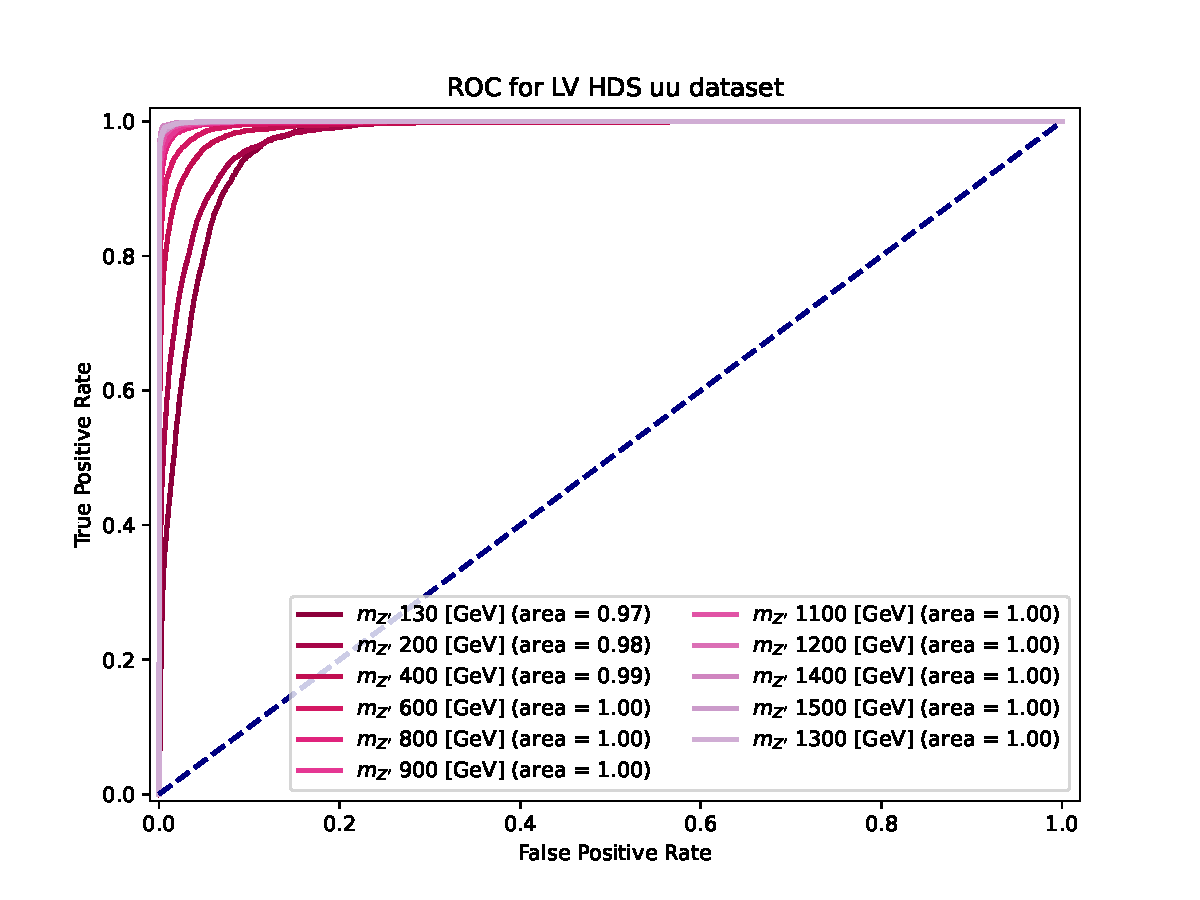
\includegraphics[width=1\textwidth]{XGBoost/LV_HDS/ROC_uu.pdf}
      \end{subfigure}
   \caption{ROC plots for every Z' mass point on network trained on Z' LV HDS}\label{fig:LV_HDS_ROCS}
\end{figure}
\\Plotting the significance of the models given the binning we get the results from Figure \ref{fig:LV_HDS_exp_sig}
\begin{figure}[!ht]
	\centering
	\begin{subfigure}[b]{0.49\textwidth}
      \centering
      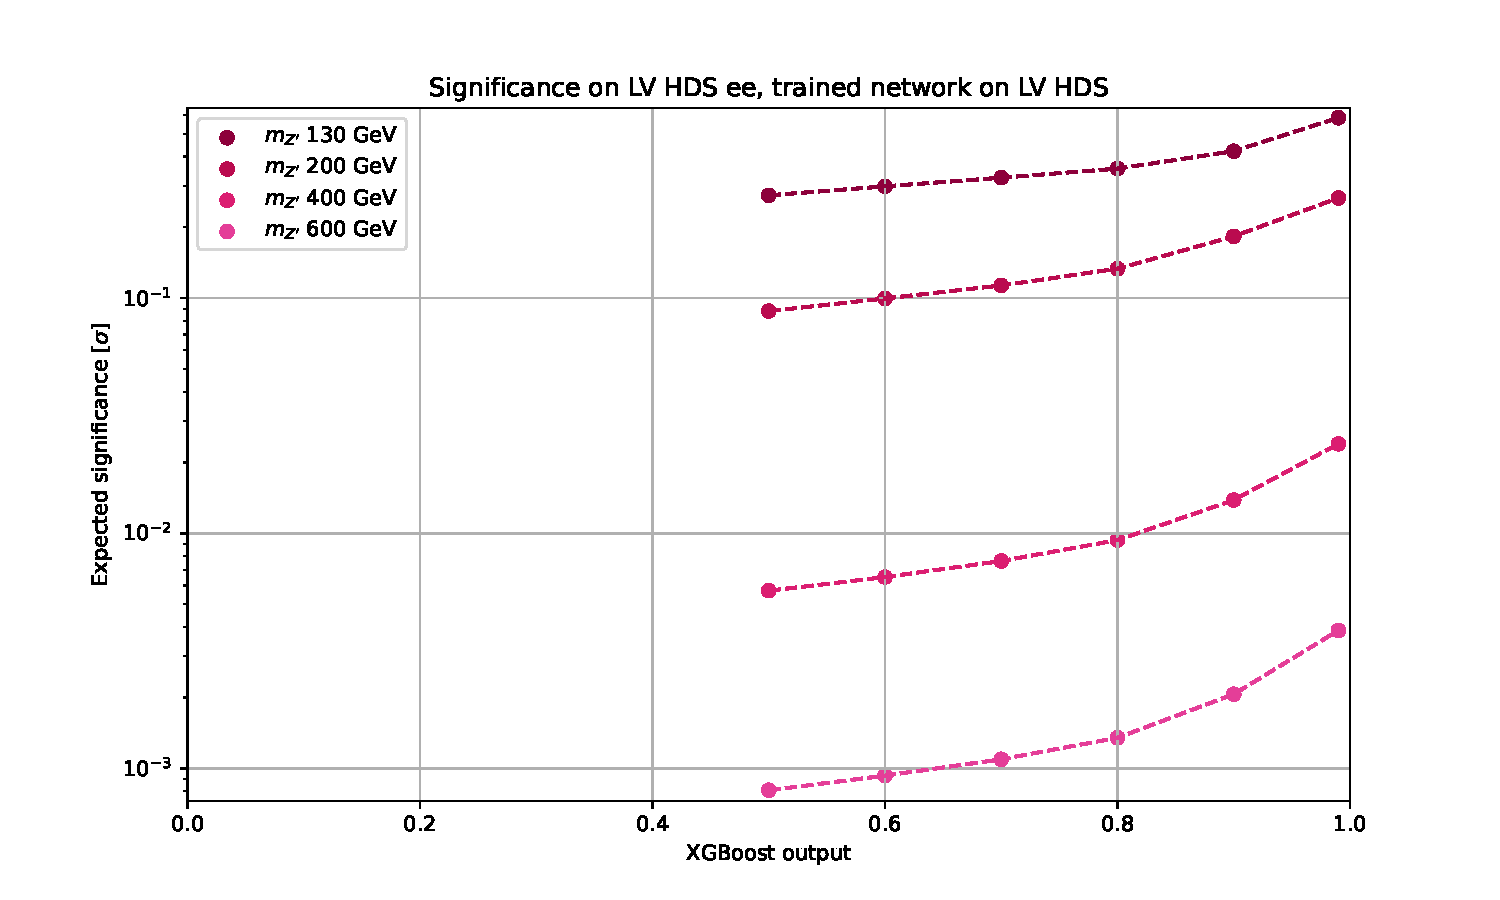
\includegraphics[width=1\textwidth]{XGBoost/LV_HDS/EXP_SIG_ee.pdf}
      \end{subfigure}
   \hfill
   \begin{subfigure}[b]{0.49\textwidth}
      \centering
      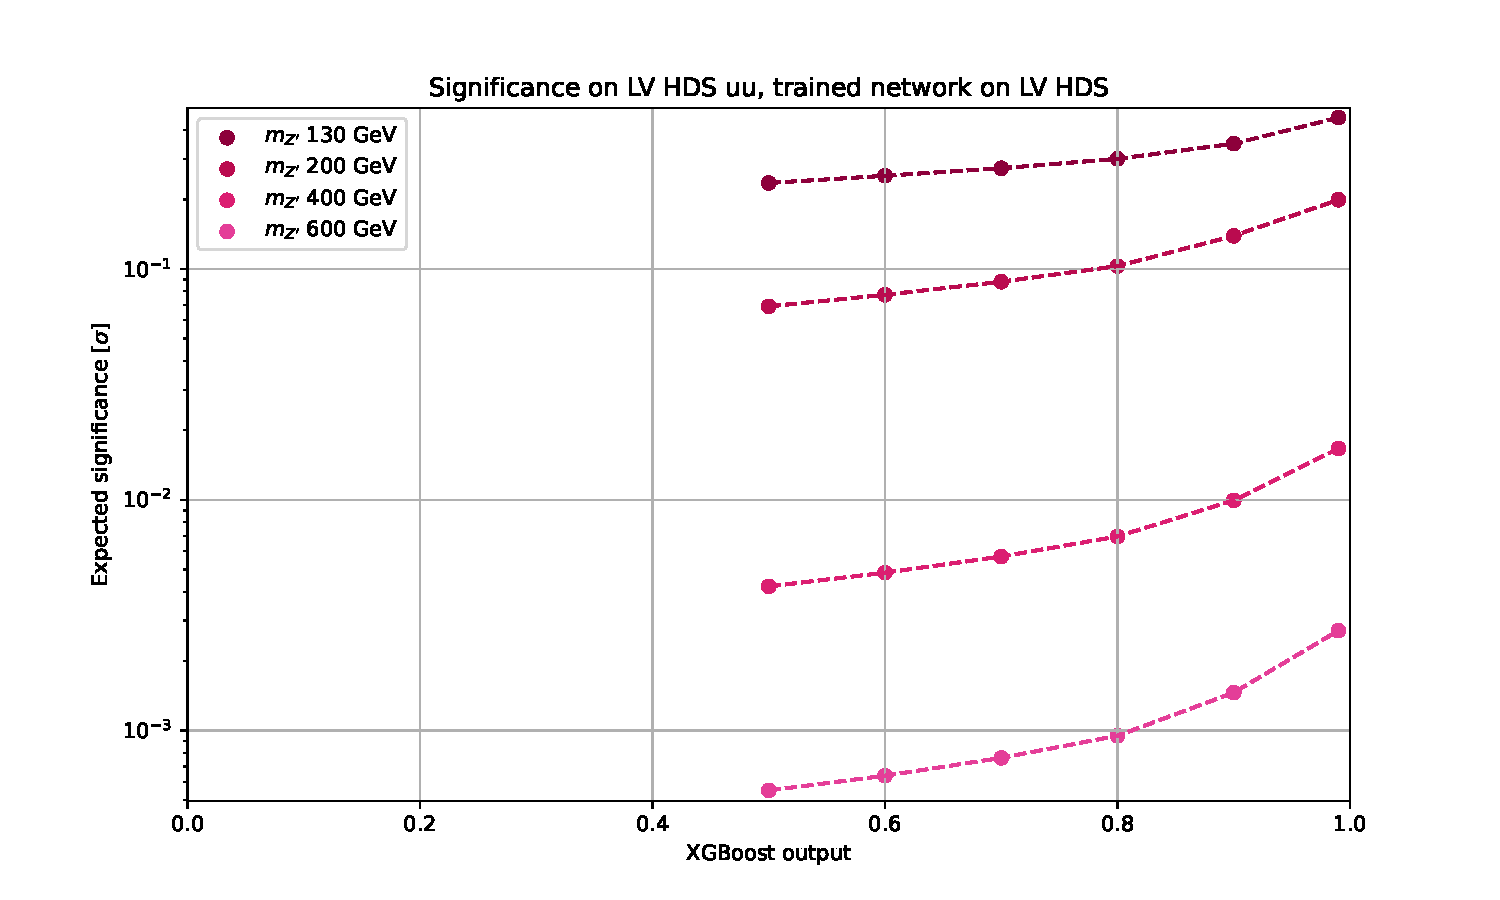
\includegraphics[width=1\textwidth]{XGBoost/LV_HDS/EXP_SIG_uu.pdf}
      \end{subfigure}
   \caption{Expected significance plots for Z' mass points on network trained on Z' LV HDS}\label{fig:LV_HDS_exp_sig}
\end{figure}
\\Using the last bin as the significance is greatest there, such that we effectively make a cut based on the BDT score. Using the last bin, we can calculate a mass exclusion for both electron and muon channel.\\
\\To do so we need to count the number of signal and background events that are on the last bin, as well as their uncertainties. Aditionally we will include the number of real data events that are there such that we can follow the 
method explained in Chapter \ref{sec:stat_anal}. In Table \ref{tab:stat_vals_LV_HDS} we see the values for each Z' mass point.
\begin{figure}[!ht]
	\centering
   \begin{subfigure}[b]{0.49\textwidth}
      \centering
      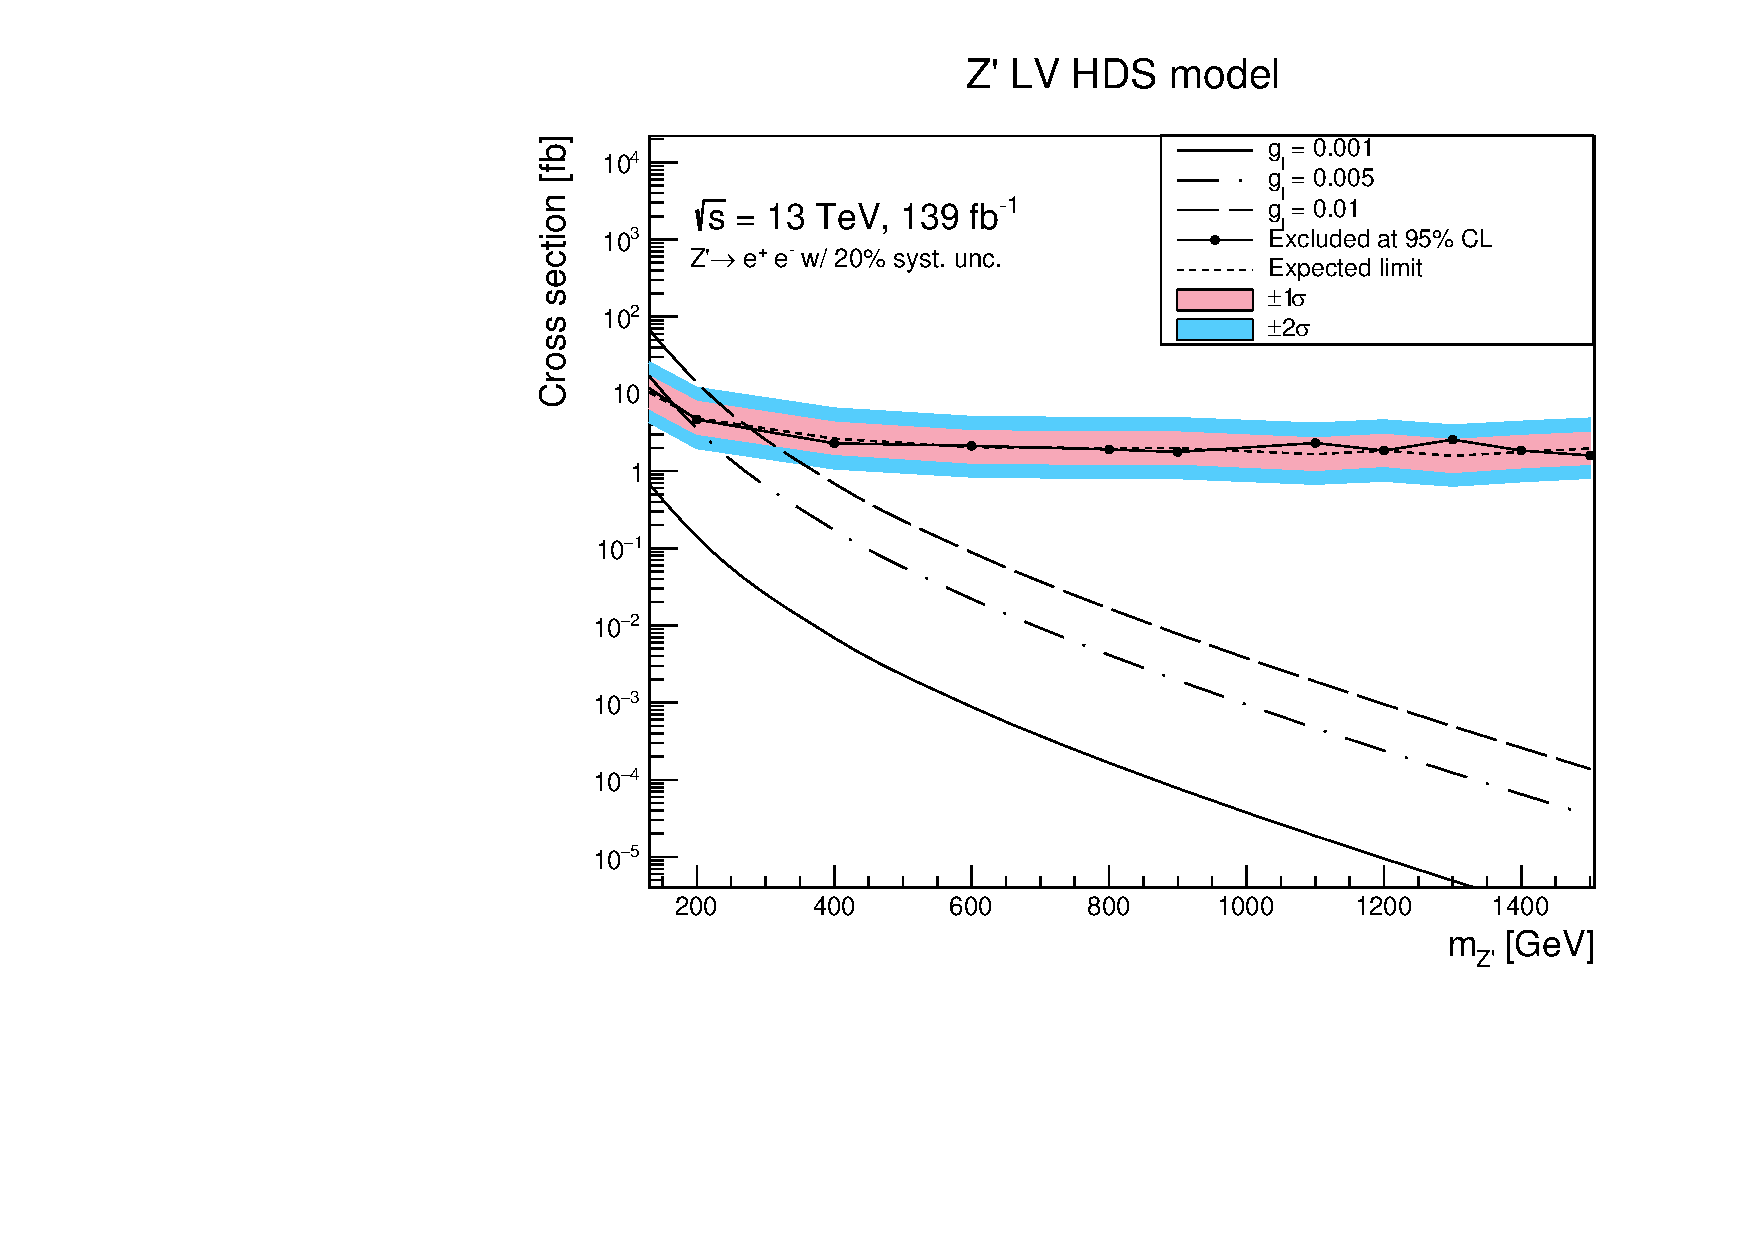
\includegraphics[width=1\textwidth]{Limits/LV_HDS/mass_exclusion_ee.pdf}
      \end{subfigure}
   \hfill
   \begin{subfigure}[b]{0.49\textwidth}
      \centering
      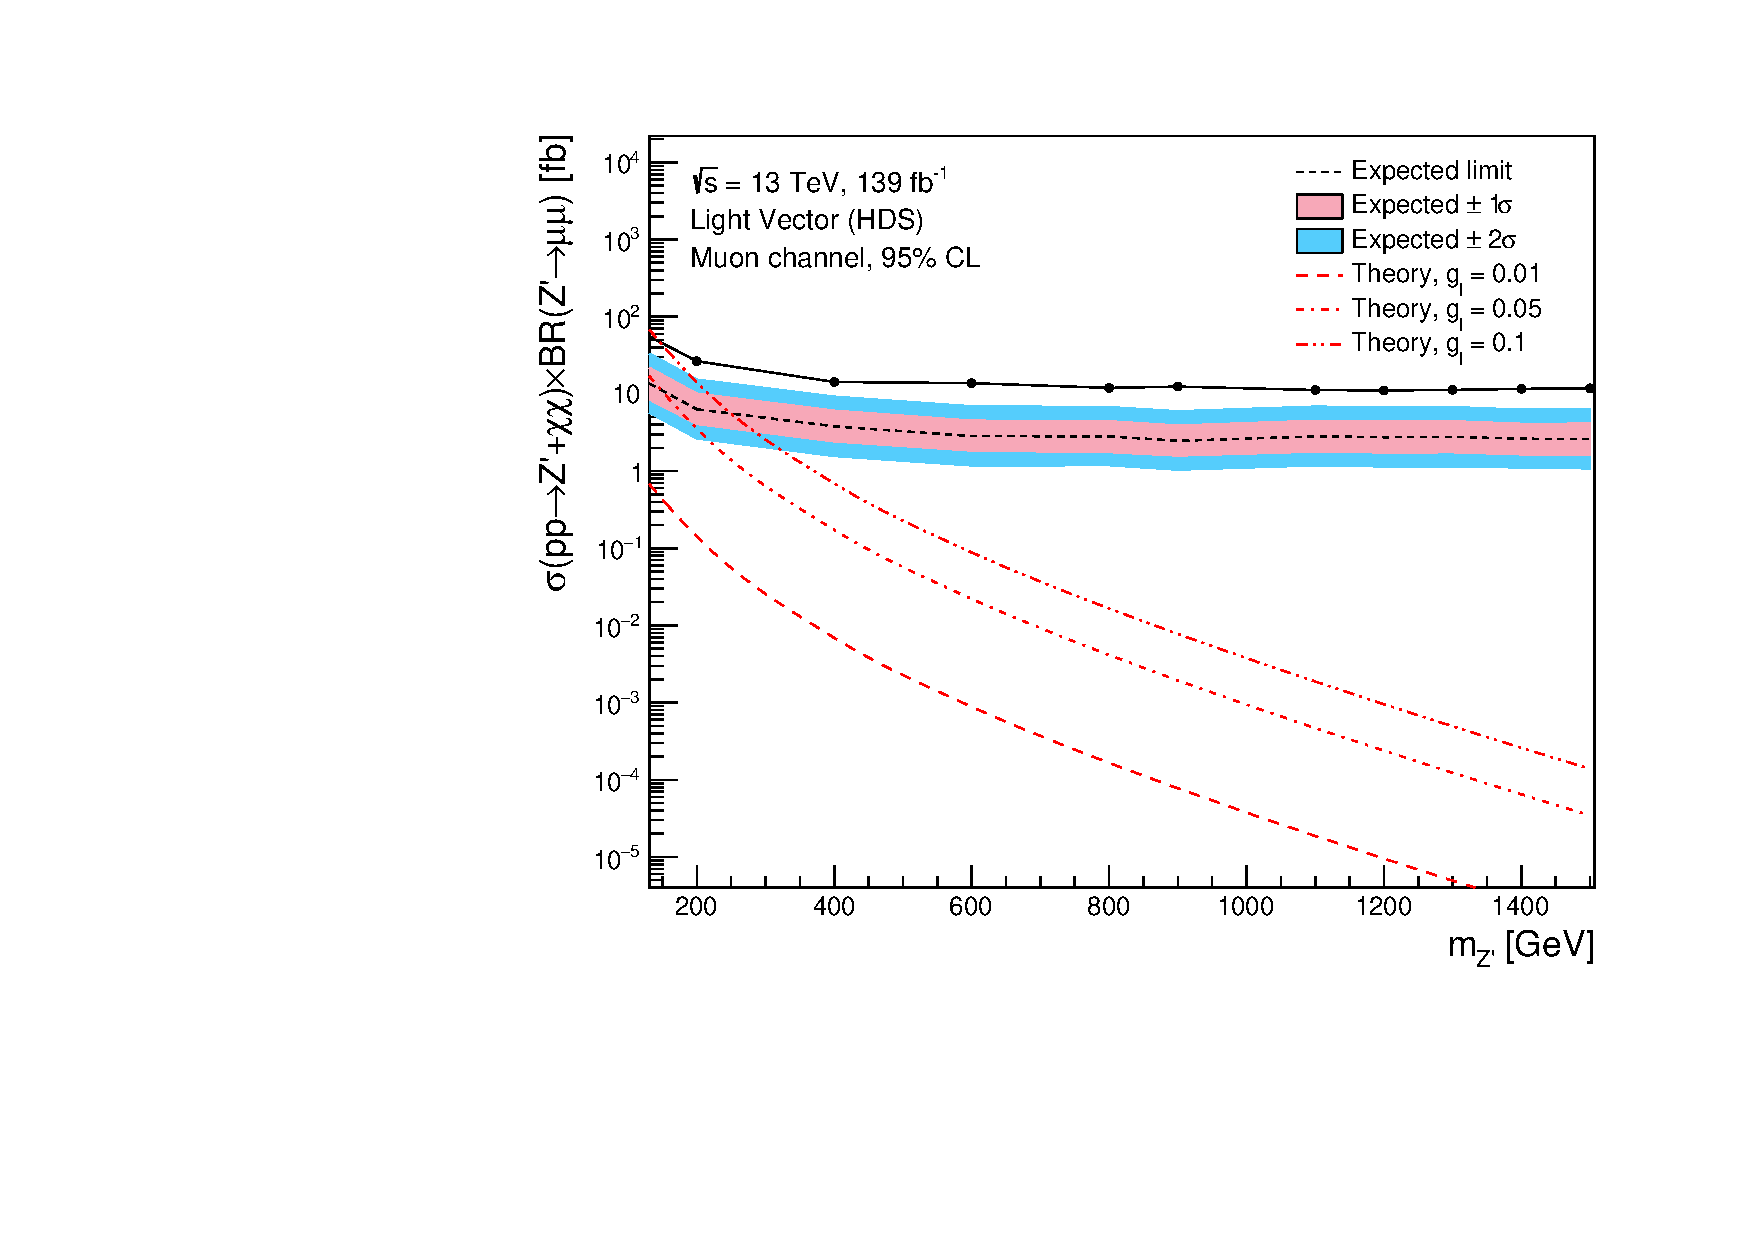
\includegraphics[width=1\textwidth]{Limits/LV_HDS/mass_exclusion_uu.pdf}
      \end{subfigure}
   \caption{Mass exclusion limits of $ee$ and $\mu\mu$ channel for all Z' LV HDS model}\label{fig:LV_HDS_exclusion_ee_uu}
\end{figure}
As the lepton coupling was chosen to be $g_l=0.001$ when simulating the data, by the assumption that the number of events that survived the cuts is the same, we can increase this coupling to see how the mass limits changes.

\newpage
\section{Light Vector Light Dark Sector}Trained a network using all of the SM background samples and every different Z' mass of this model. Here are the results
\begin{figure}[!ht]
	\centering
	\begin{subfigure}[b]{0.49\textwidth}
      \centering
      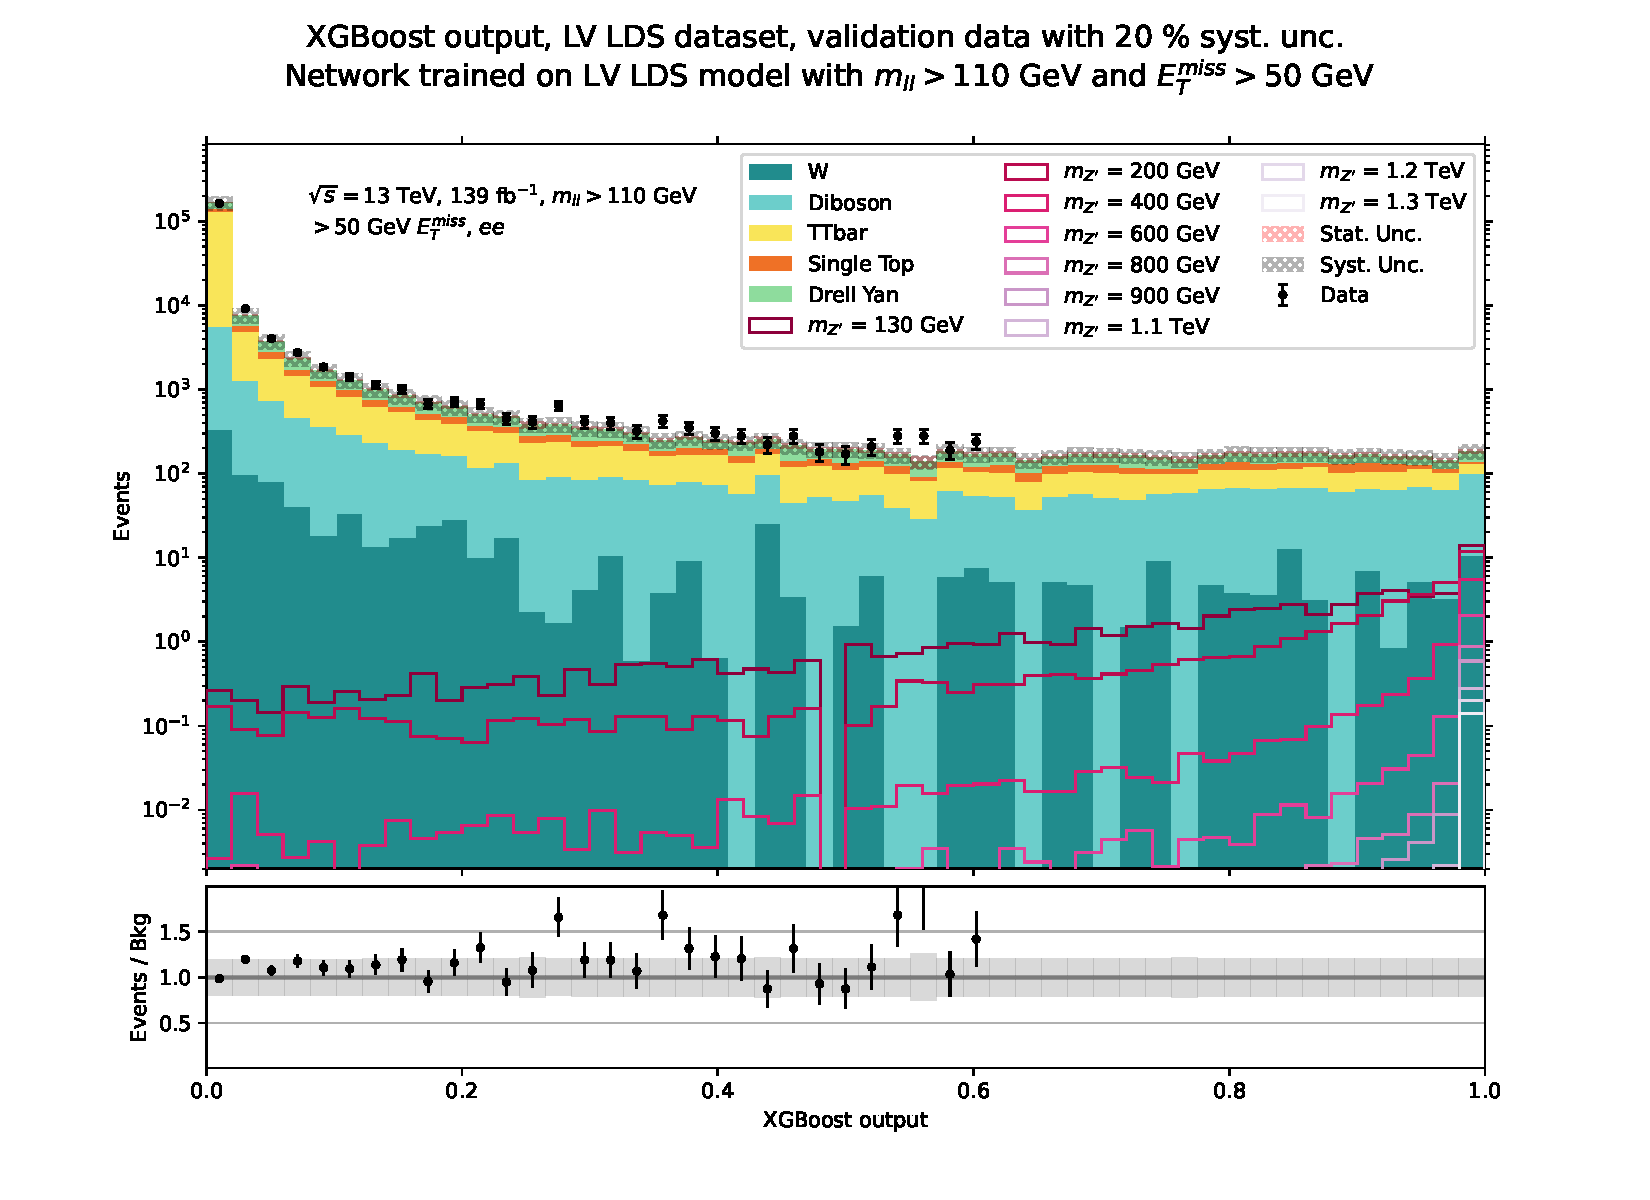
\includegraphics[width=1\textwidth]{XGBoost/LV_LDS/VAL_ee.pdf}
      \end{subfigure}
   \hfill
   \begin{subfigure}[b]{0.49\textwidth}
      \centering
      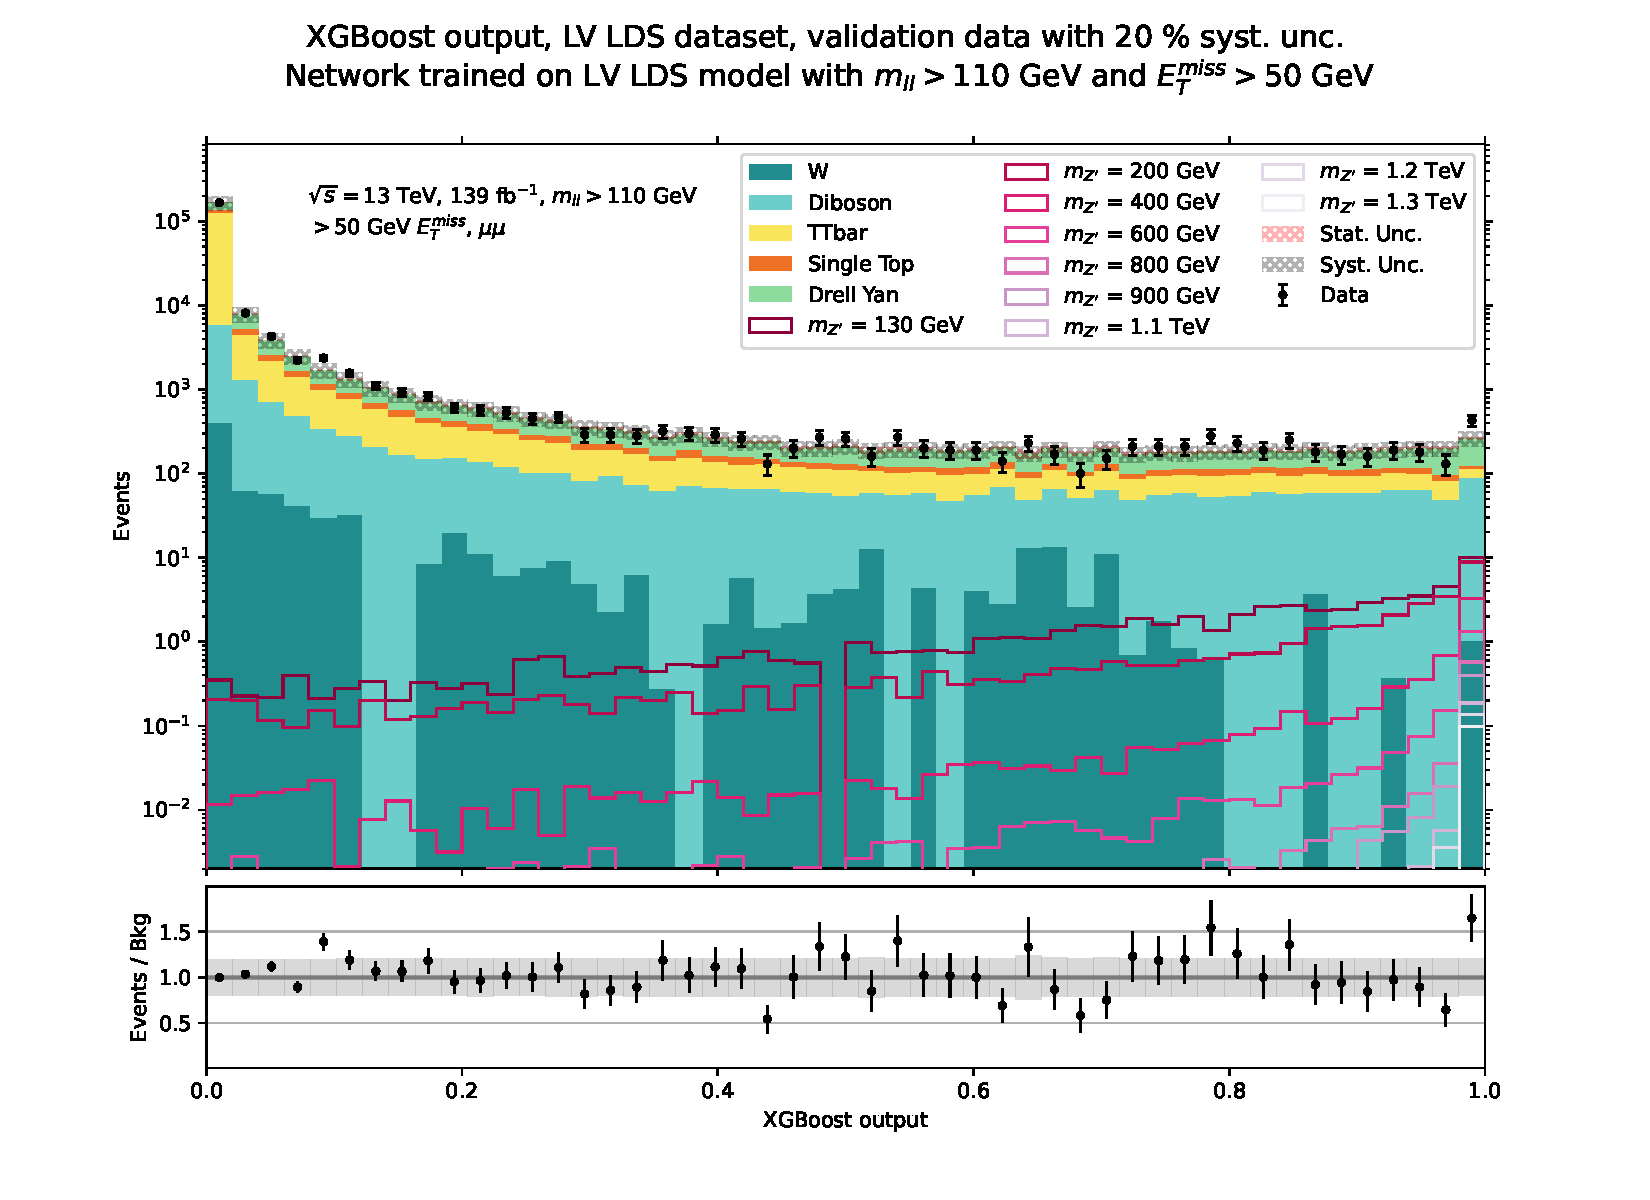
\includegraphics[width=1\textwidth]{XGBoost/LV_LDS/VAL_uu.pdf}
      \end{subfigure}
   \caption{Validation plots for network trained on Z' LV LDS}\label{fig:LV_LDS_vals}
\end{figure}
\\With the ROC for each mass point seen in Figure \ref{fig:LV_LDS_ROCS}.
\begin{figure}[!ht]
	\centering
	\begin{subfigure}[b]{0.49\textwidth}
      \centering
      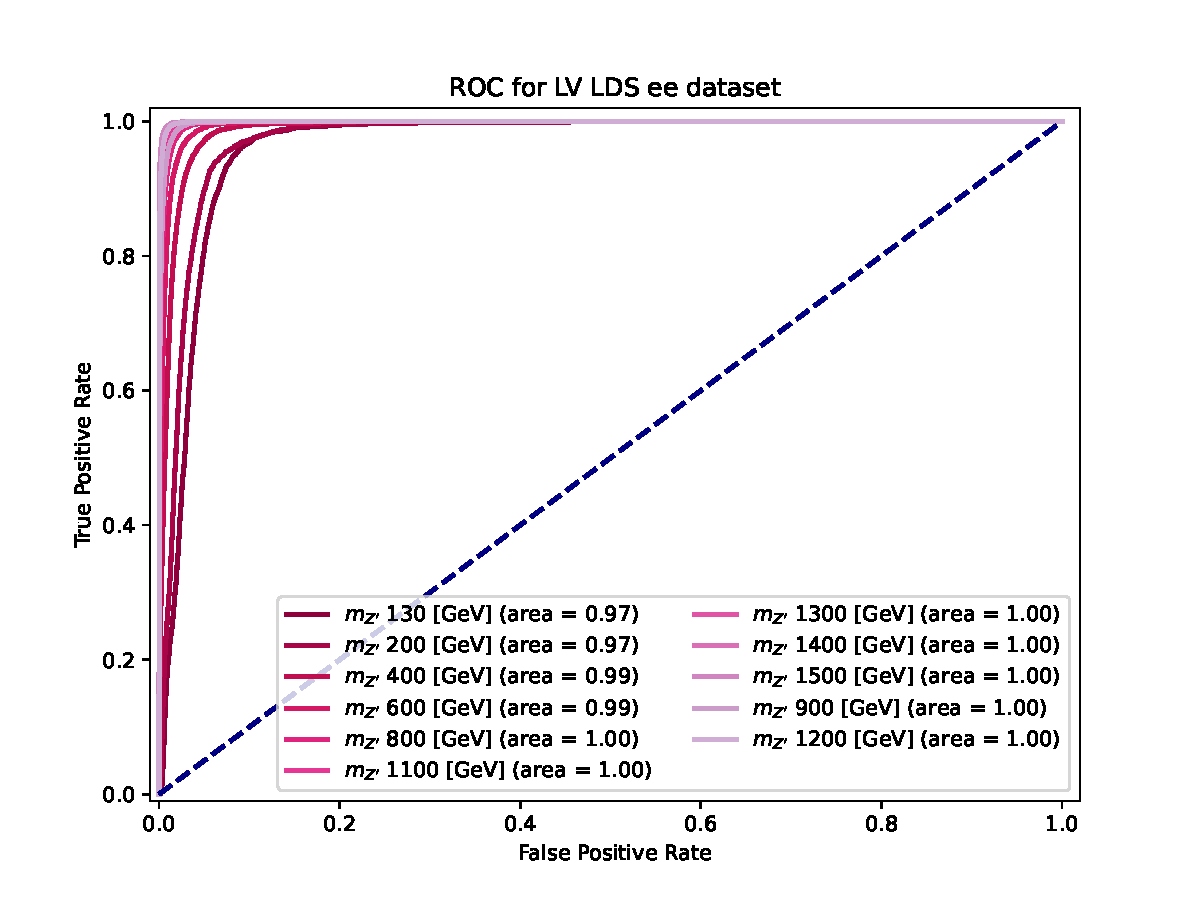
\includegraphics[width=1\textwidth]{XGBoost/LV_LDS/ROC_ee.pdf}
      \end{subfigure}
   \hfill
   \begin{subfigure}[b]{0.49\textwidth}
      \centering
      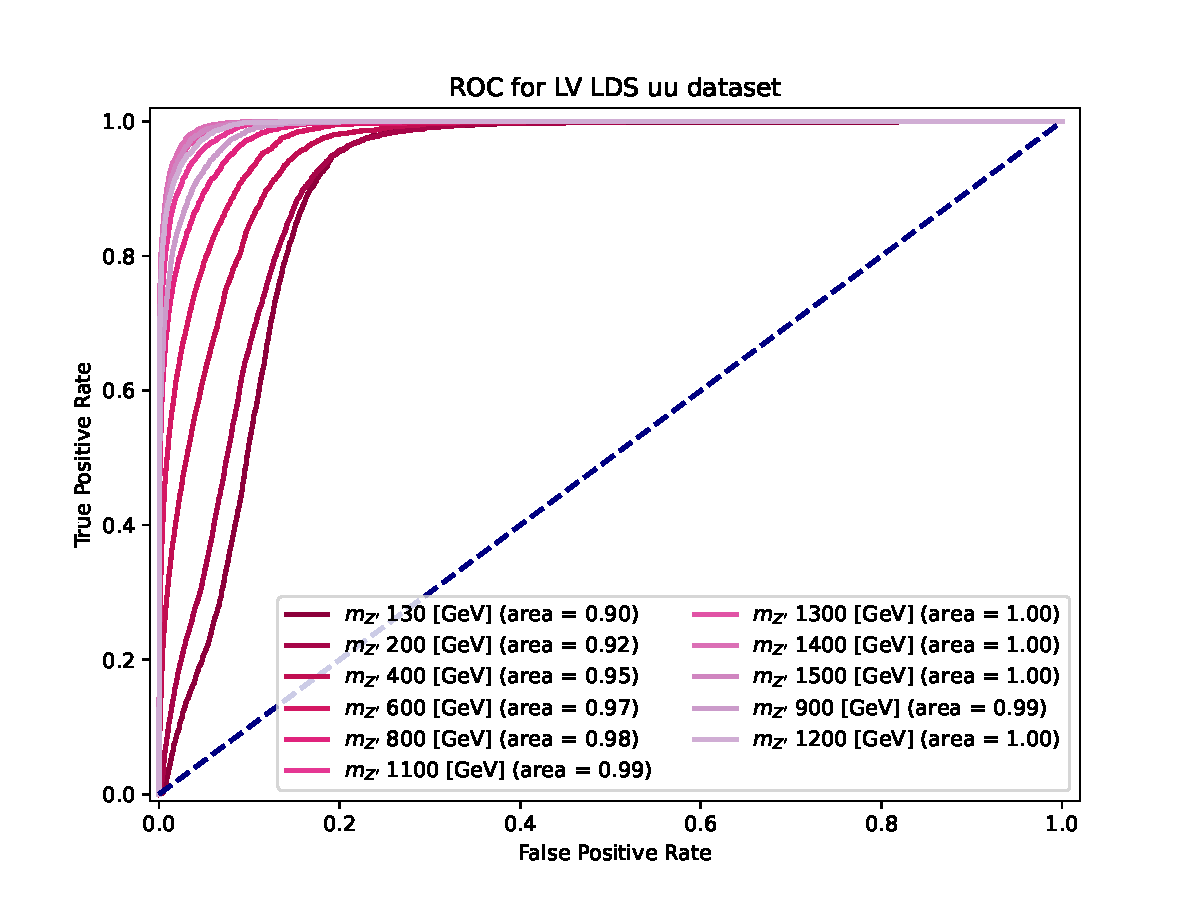
\includegraphics[width=1\textwidth]{XGBoost/LV_LDS/ROC_uu.pdf}
      \end{subfigure}
   \caption{ROC plots for every Z' mass point on network trained on Z' LV LDS}\label{fig:LV_LDS_ROCS}
\end{figure}
\\Plotting the significance of the models given the binning we get the results from Figure \ref{fig:LV_LDS_exp_sig}
\begin{figure}[!ht]
	\centering
	\begin{subfigure}[b]{0.49\textwidth}
      \centering
      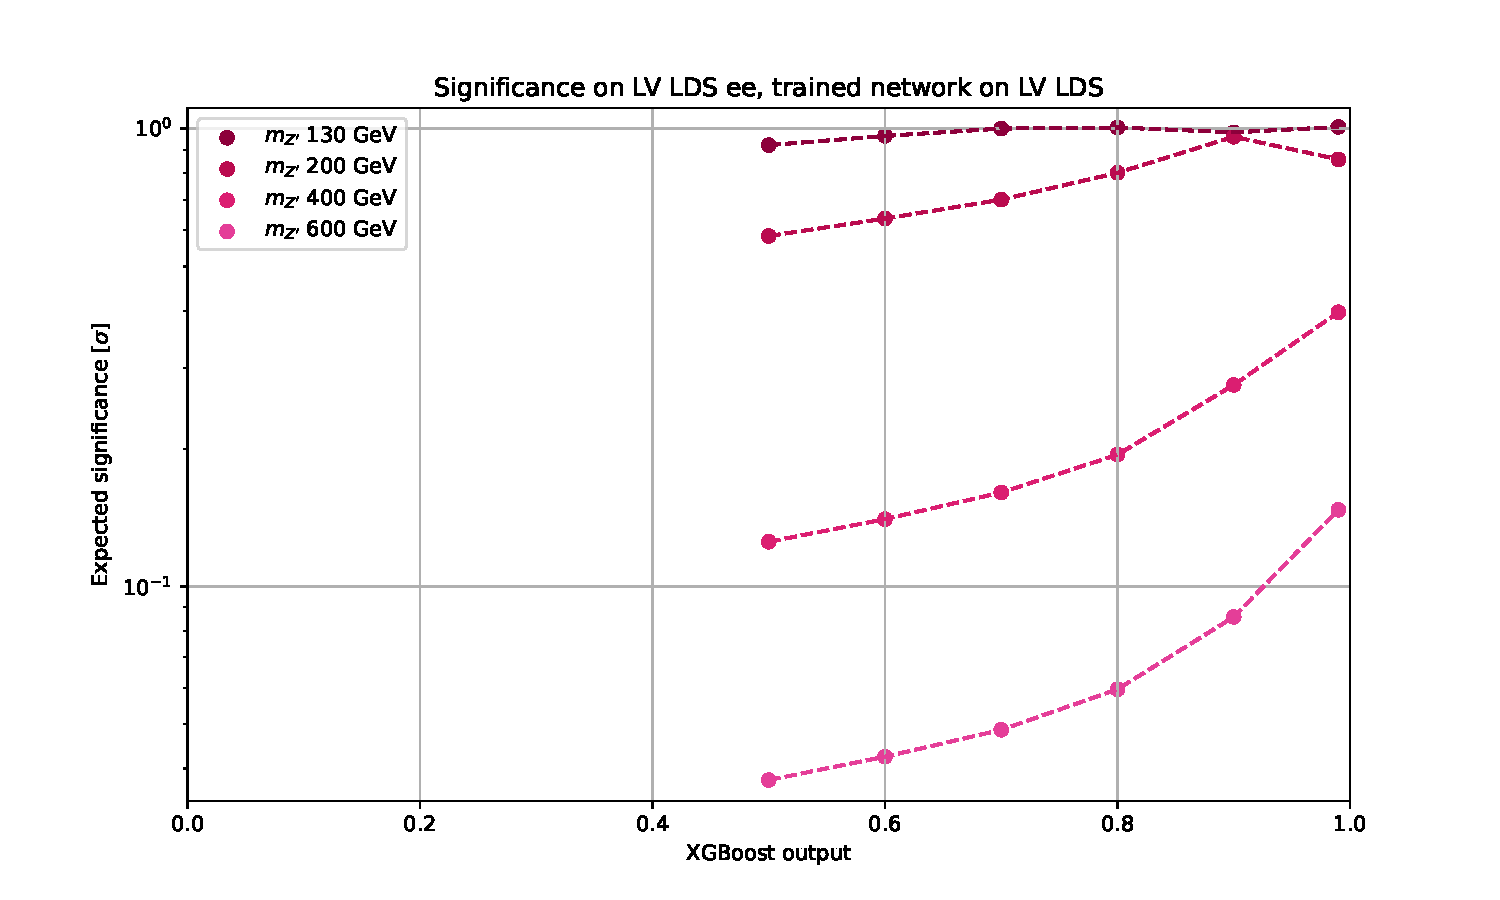
\includegraphics[width=1\textwidth]{XGBoost/LV_LDS/EXP_SIG_ee.pdf}
      \end{subfigure}
   \hfill
   \begin{subfigure}[b]{0.49\textwidth}
      \centering
      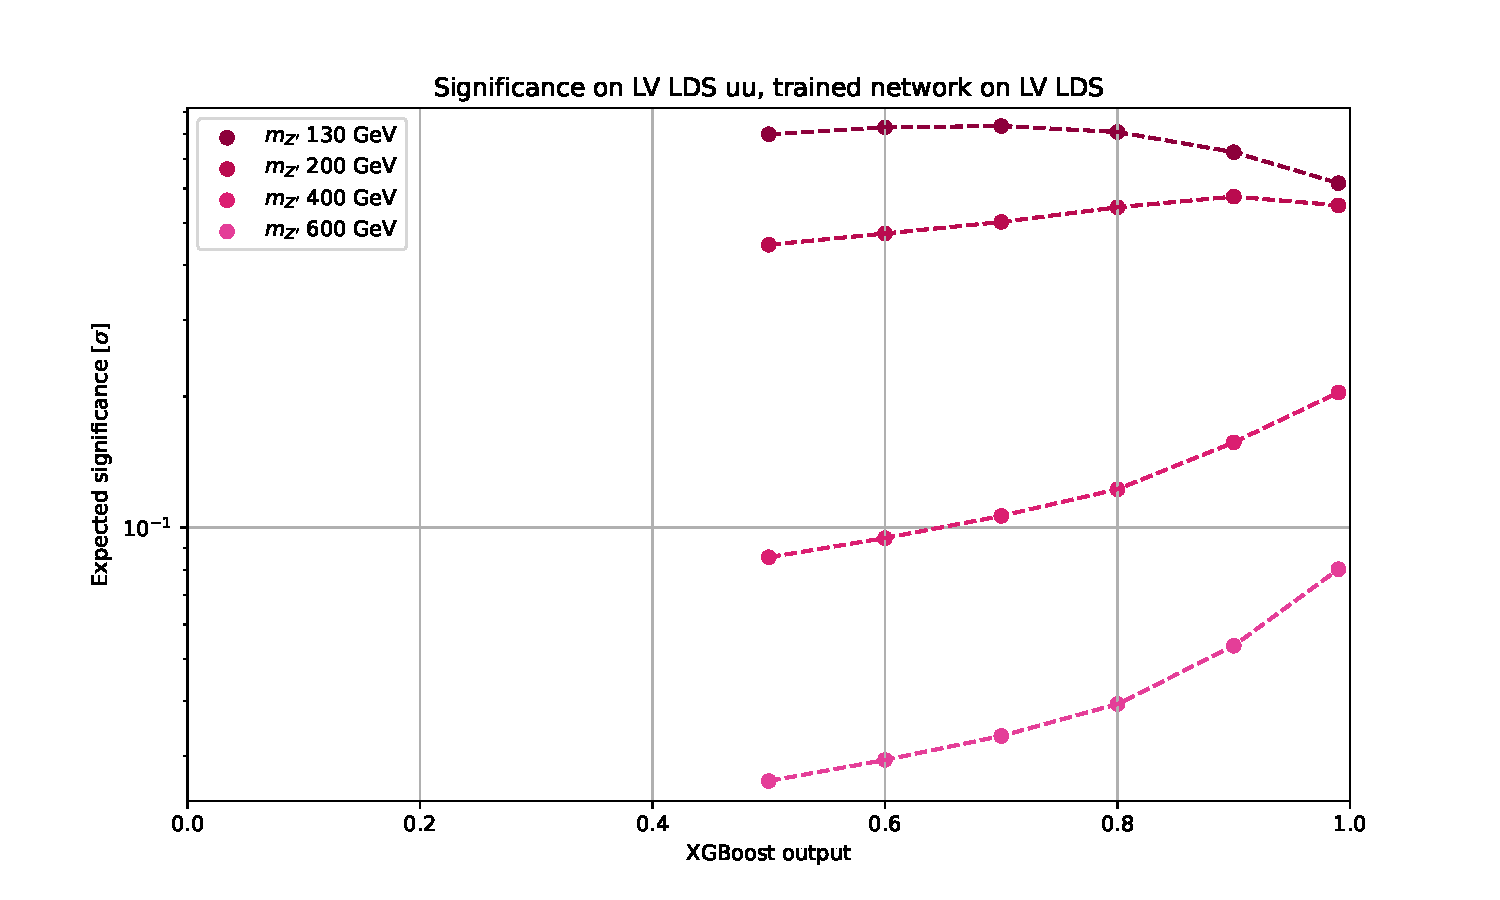
\includegraphics[width=1\textwidth]{XGBoost/LV_LDS/EXP_SIG_uu.pdf}
      \end{subfigure}
   \caption{Expected significance plots for Z' mass points on network trained on Z' LV LDS}\label{fig:LV_LDS_exp_sig}
\end{figure}
\\Using the last bin as the significance is greatest there, such that we effectively make a cut based on the BDT score. Using the last bin, we can calculate a mass exclusion for both electron and muon channel.\\
\\To do so we need to count the number of signal and background events that are on the last bin, as well as their uncertainties. Aditionally we will include the number of real data events that are there such that we can follow the 
method explained in Chapter \ref{sec:stat_anal}. In Table \ref{tab:stat_vals_LV_LDS} we see the values for each Z' mass point.
\begin{figure}[!ht]
	\centering
   \begin{subfigure}[b]{0.49\textwidth}
      \centering
      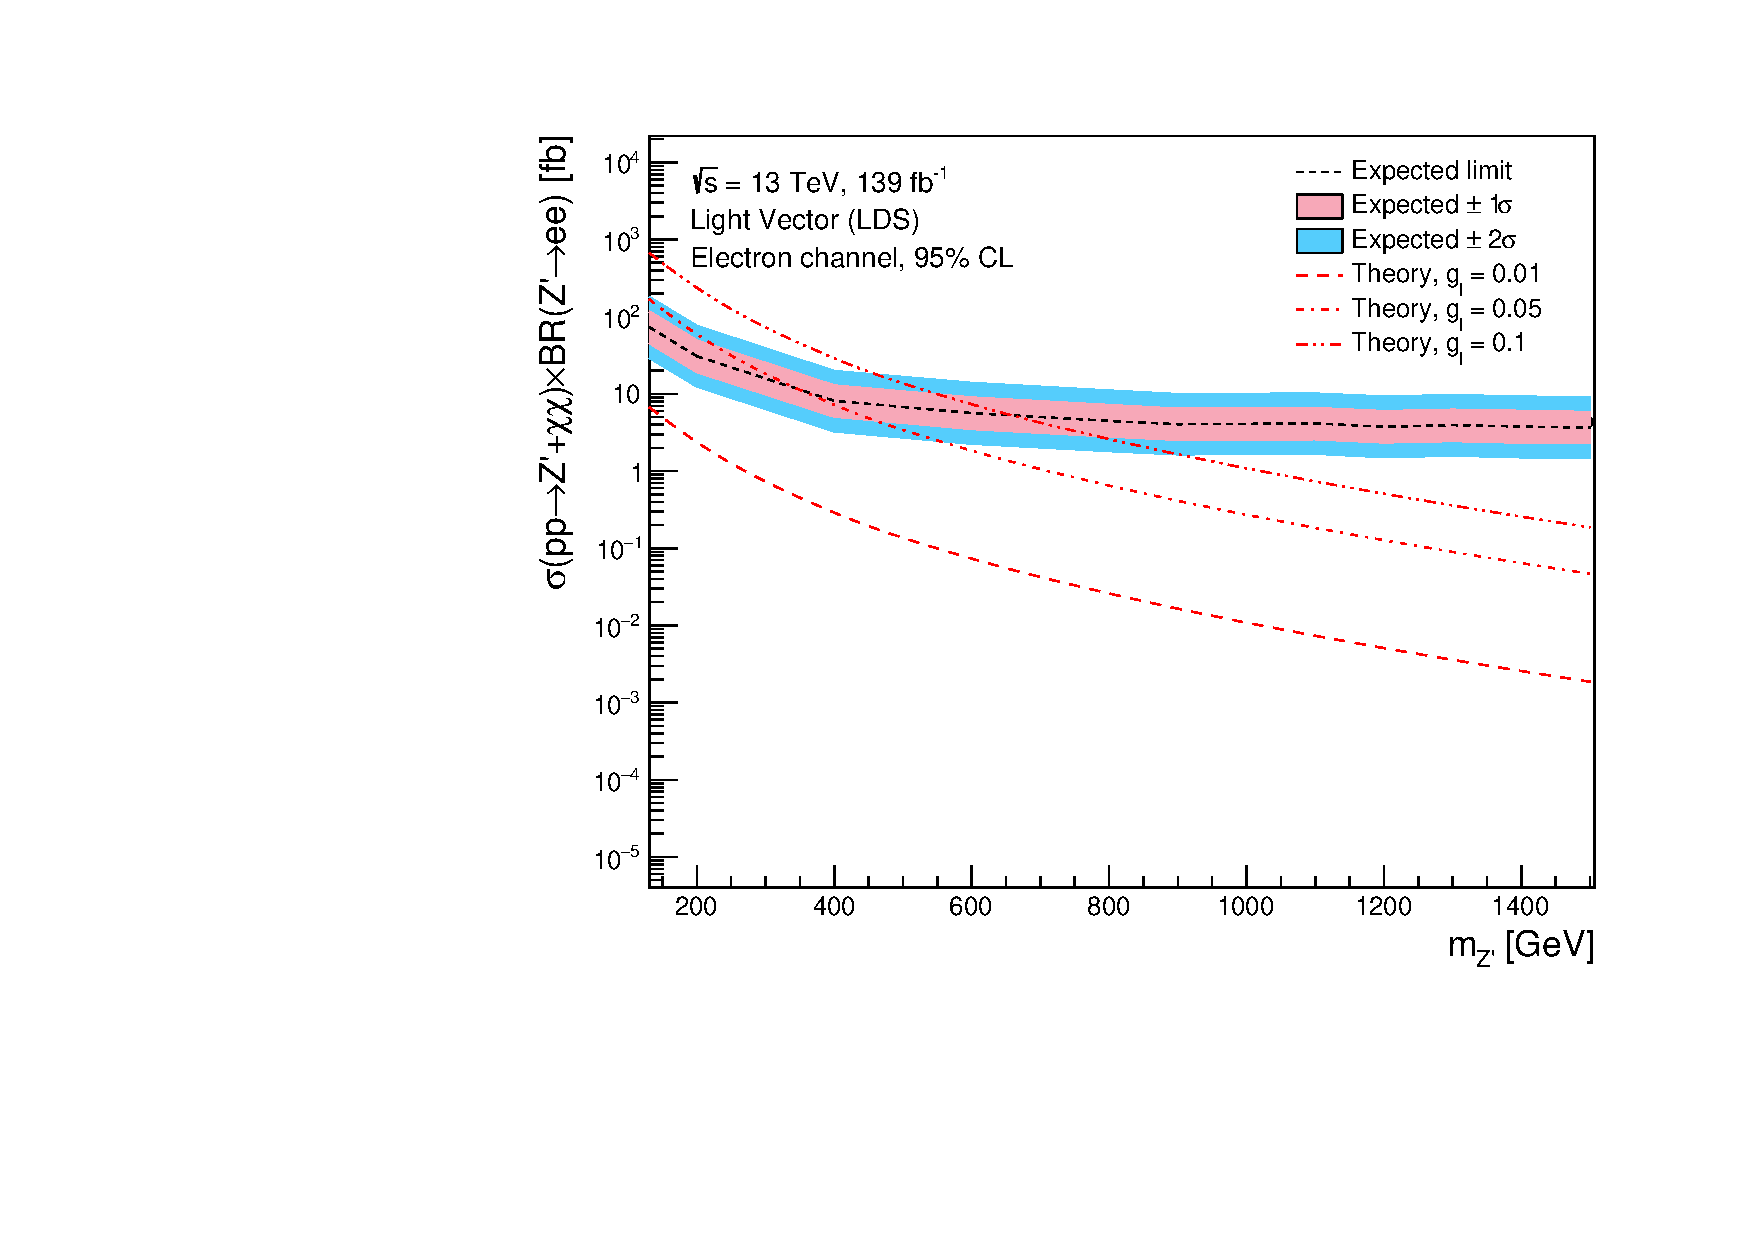
\includegraphics[width=1\textwidth]{Limits/LV_LDS/mass_exclusion_ee.pdf}
      \end{subfigure}
   \hfill
   \begin{subfigure}[b]{0.49\textwidth}
      \centering
      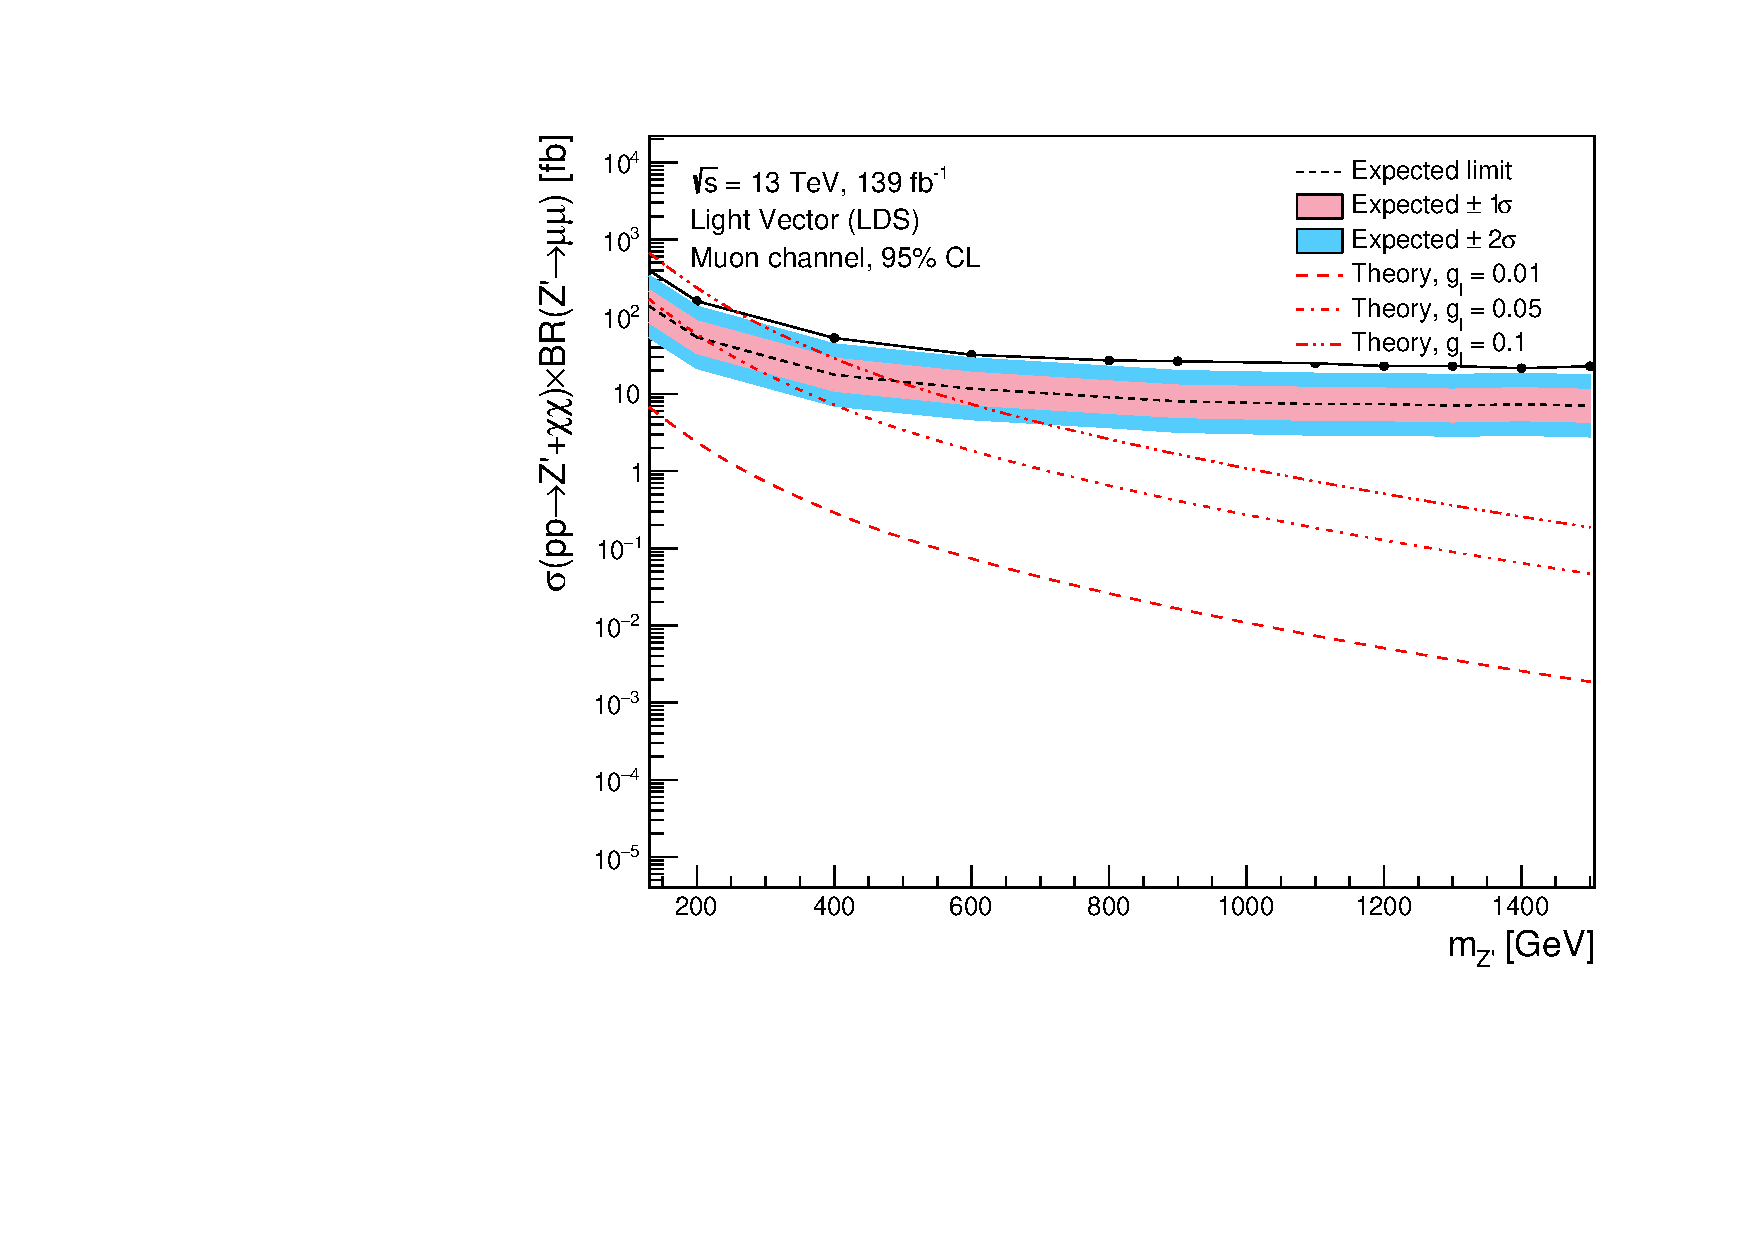
\includegraphics[width=1\textwidth]{Limits/LV_LDS/mass_exclusion_uu.pdf}
      \end{subfigure}
   \caption{Mass exclusion limits of $ee$ and $\mu\mu$ channel for all Z' LV LDS model}\label{fig:LV_LDS_exclusion_ee_uu}
\end{figure}
As the lepton coupling was chosen to be $g_l=0.001$ when simulating the data, by the assumption that the number of events that survived the cuts is the same, we can increase this coupling to see how the mass limits changes.


\newpage
\section{Effective Field Theory Heavy Dark Sector}Trained a network using all of the SM background samples and every different Z' mass of this model. Here are the results
% \begin{figure}[!ht]
% 	\centering
% 	\begin{subfigure}[b]{0.49\textwidth}
%       \centering
%       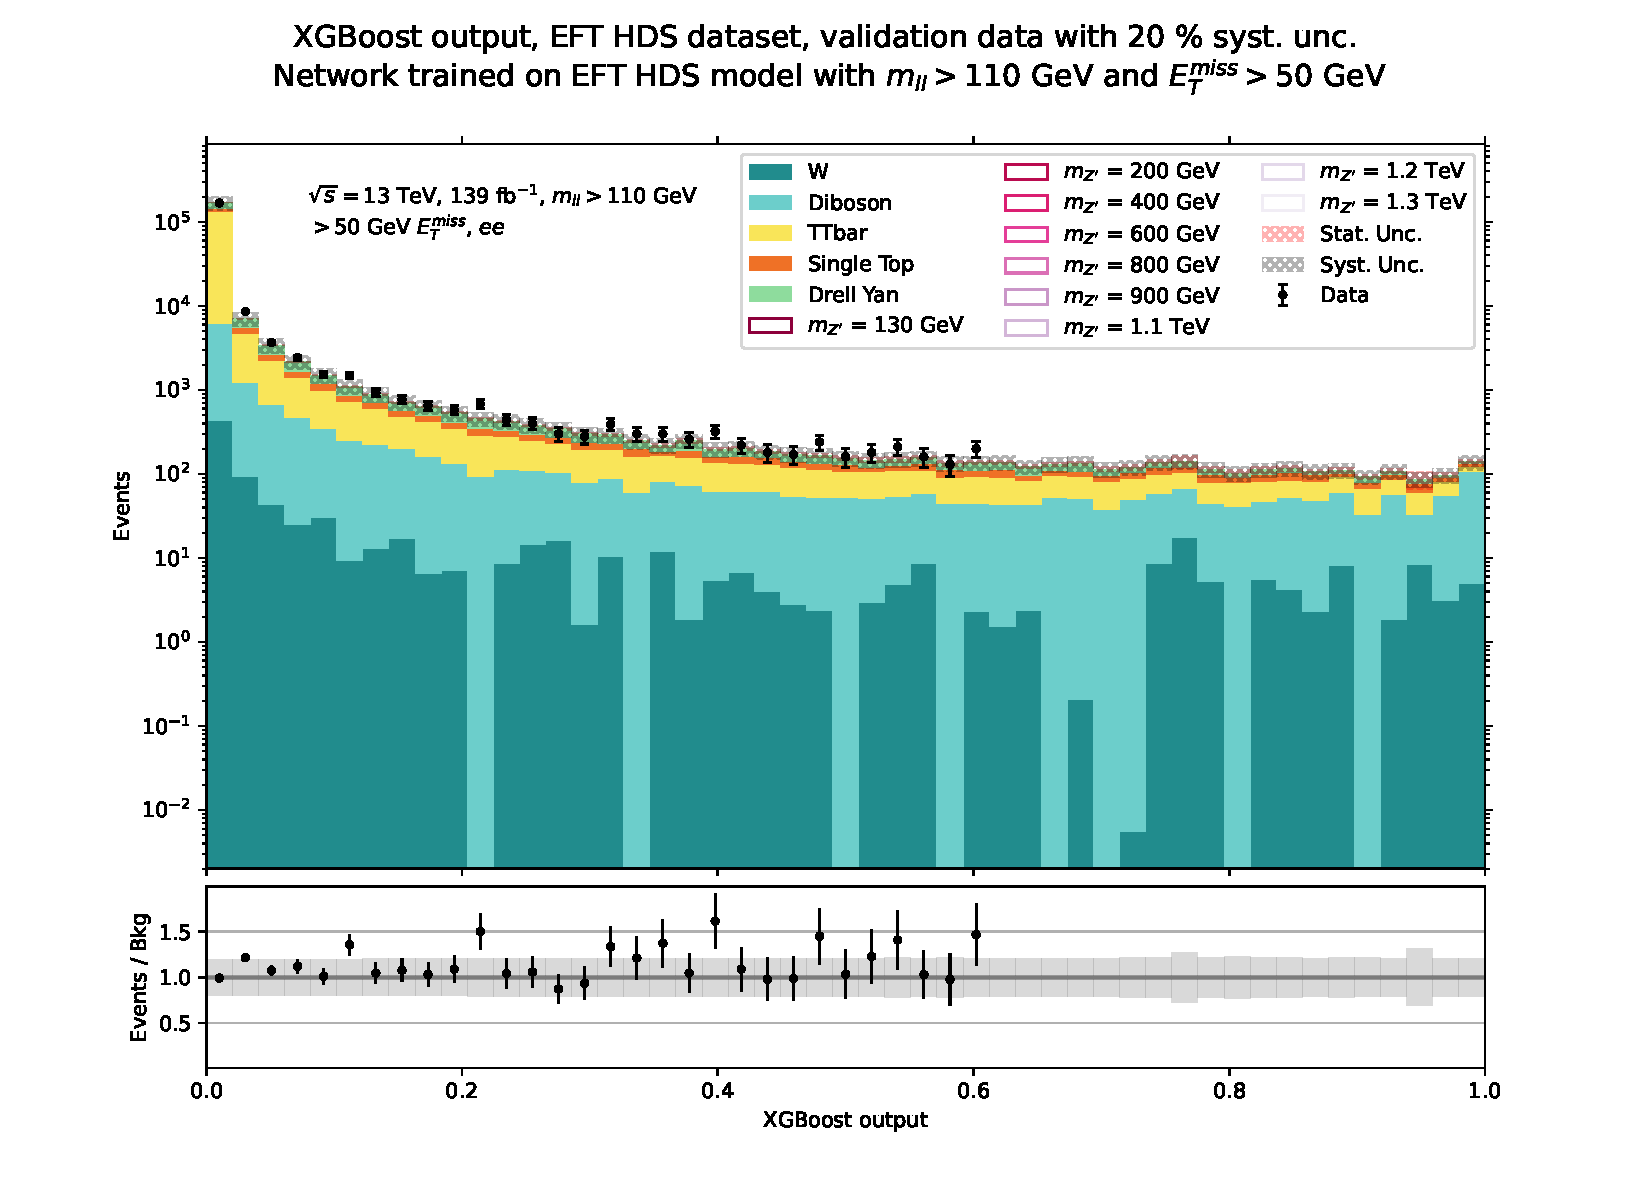
\includegraphics[width=1\textwidth]{XGBoost/EFT_HDS/VAL_ee.pdf}
%       \end{subfigure}
%    \hfill
%    \begin{subfigure}[b]{0.49\textwidth}
%       \centering
%       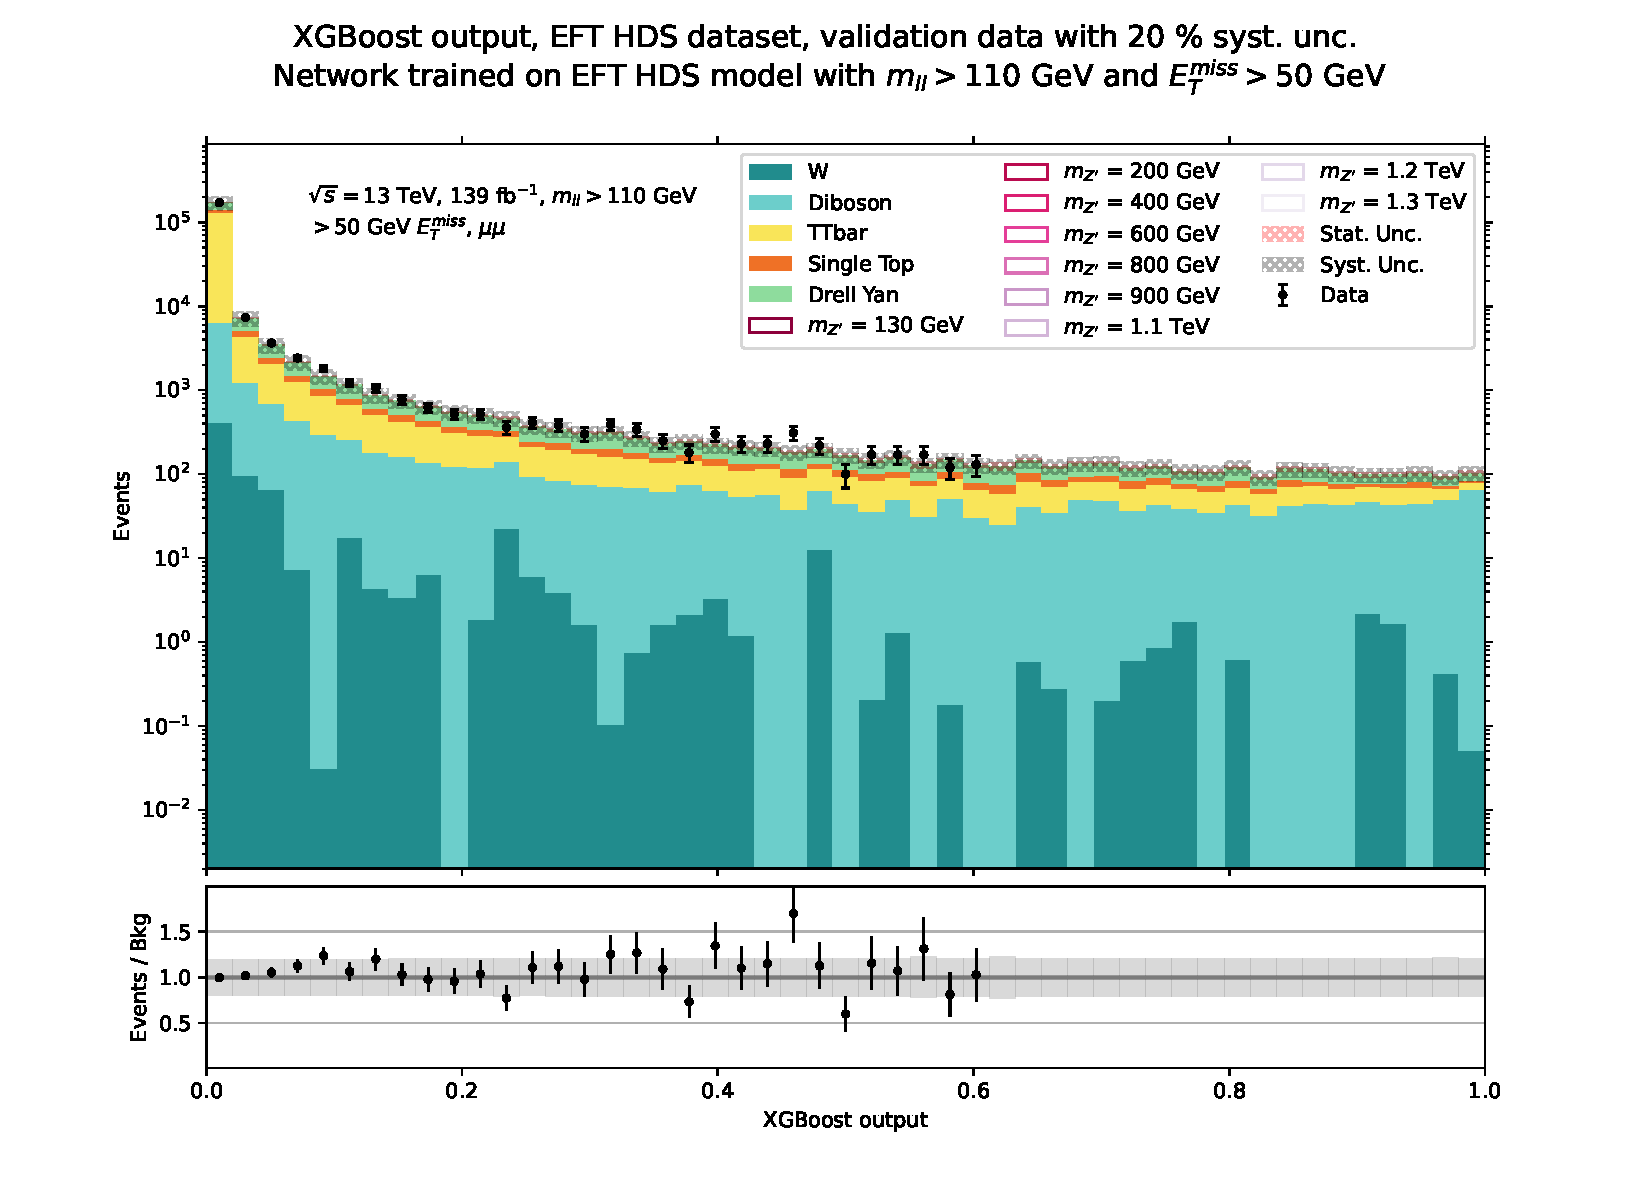
\includegraphics[width=1\textwidth]{XGBoost/EFT_HDS/VAL_uu.pdf}
%       \end{subfigure}
%    \caption{Validation plots for network trained on Z' EFT HDS}\label{fig:EFT_HDS_vals}
% \end{figure}
\\With the ROC for each mass point seen in Figure \ref{fig:EFT_HDS_ROCS}.
\begin{figure}[!ht]
	\centering
	\begin{subfigure}[b]{0.49\textwidth}
      \centering
      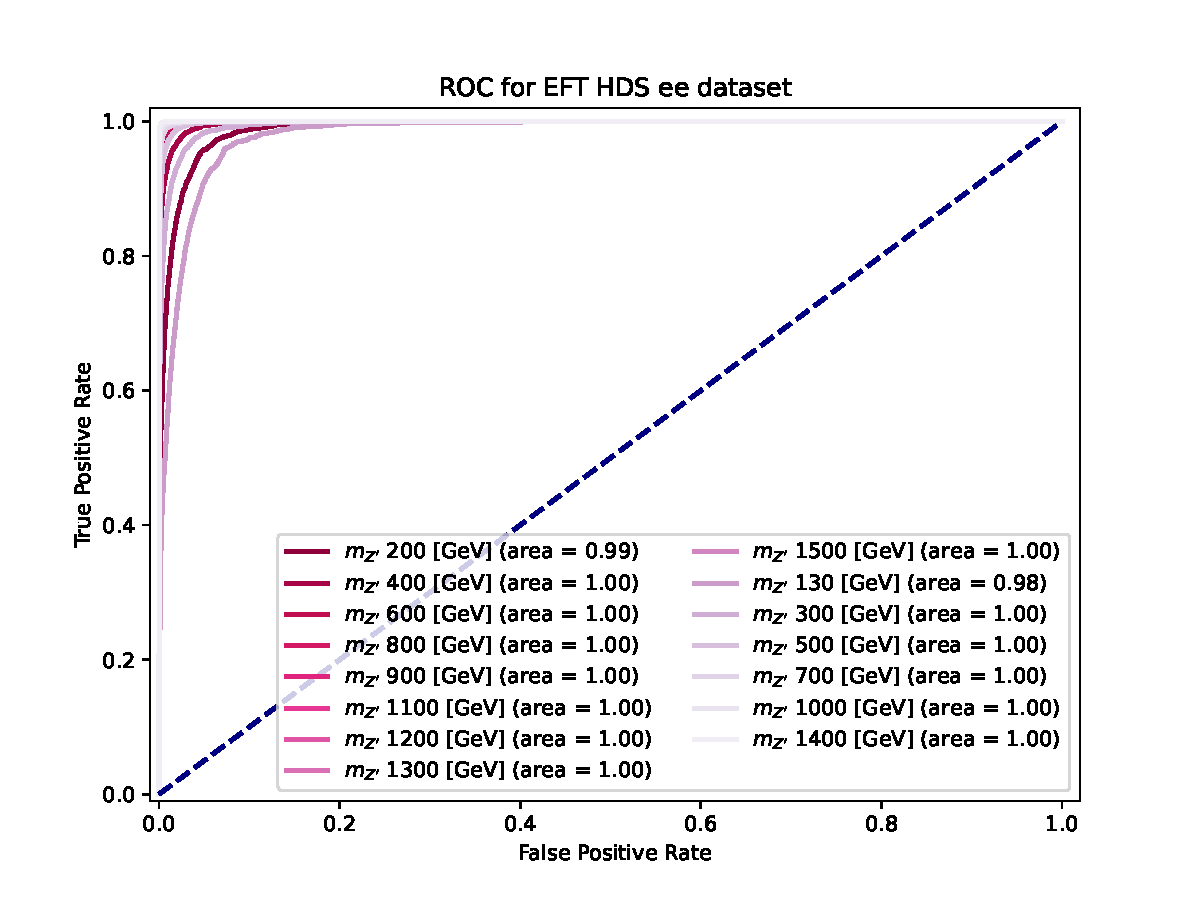
\includegraphics[width=1\textwidth]{XGBoost/EFT_HDS/ROC_ee.pdf}
      \end{subfigure}
   \hfill
   \begin{subfigure}[b]{0.49\textwidth}
      \centering
      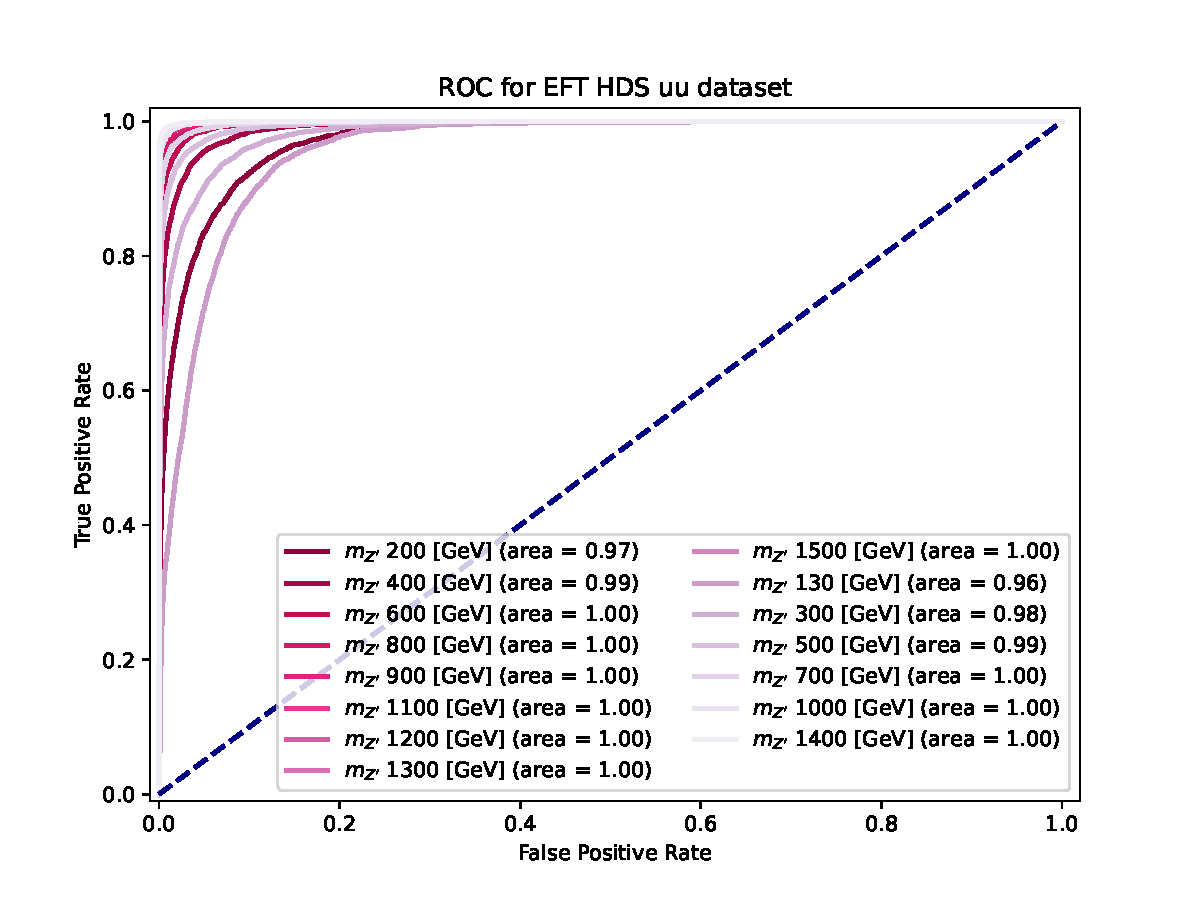
\includegraphics[width=1\textwidth]{XGBoost/EFT_HDS/ROC_uu.pdf}
      \end{subfigure}
   \caption{ROC plots for every Z' mass point on network trained on Z' EFT HDS}\label{fig:EFT_HDS_ROCS}
\end{figure}
\\Plotting the significance of the models given the binning we get the results from Figure \ref{fig:EFT_HDS_exp_sig}
\begin{figure}[!ht]
	\centering
	\begin{subfigure}[b]{0.49\textwidth}
      \centering
      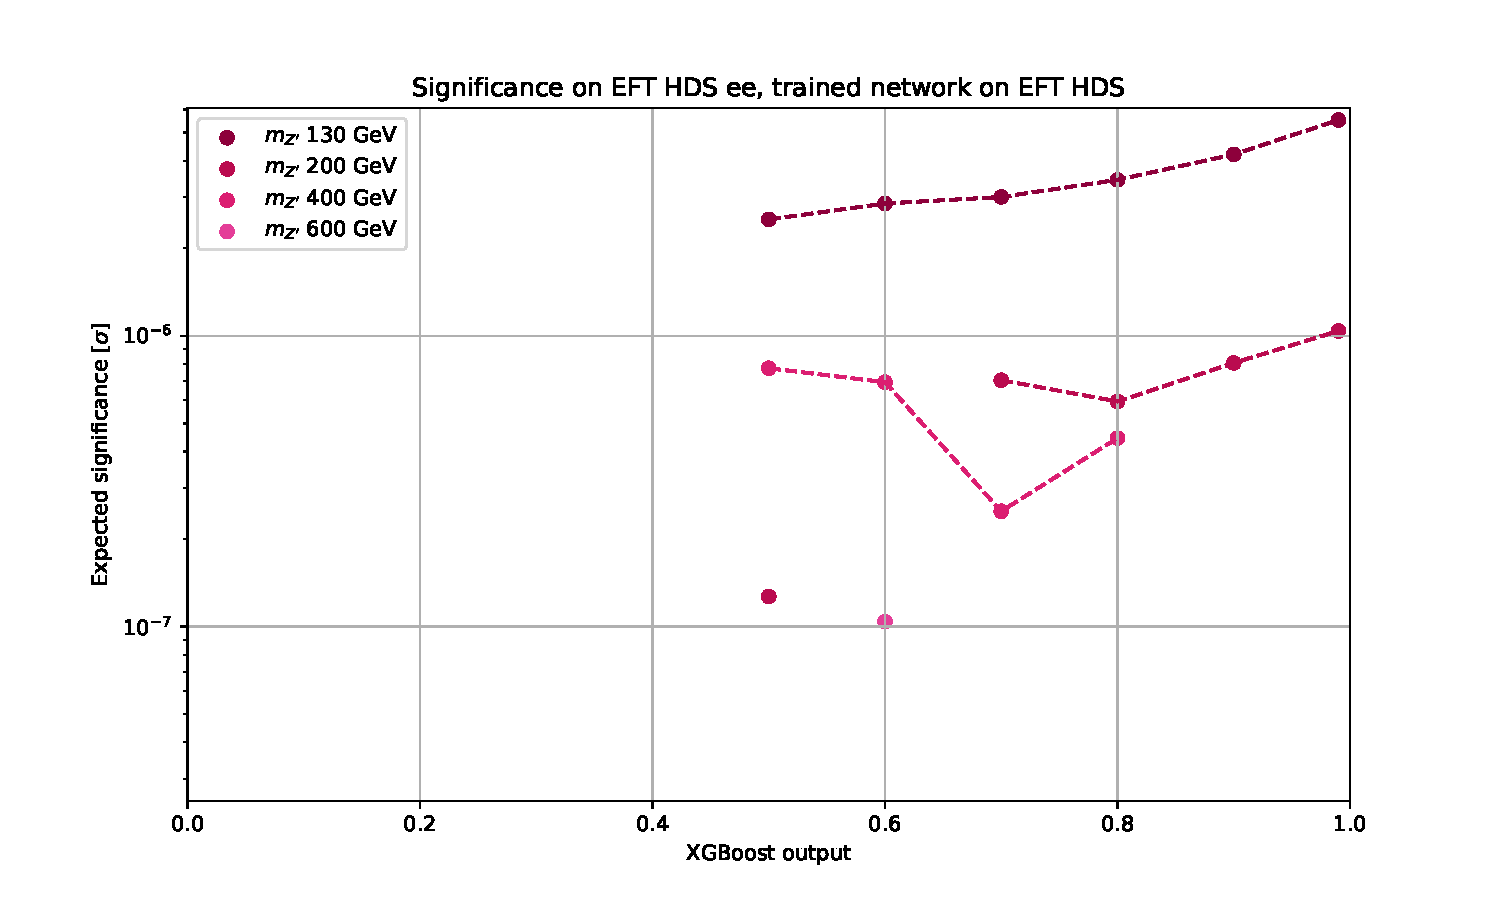
\includegraphics[width=1\textwidth]{XGBoost/EFT_HDS/EXP_SIG_ee.pdf}
      \end{subfigure}
   \hfill
   \begin{subfigure}[b]{0.49\textwidth}
      \centering
      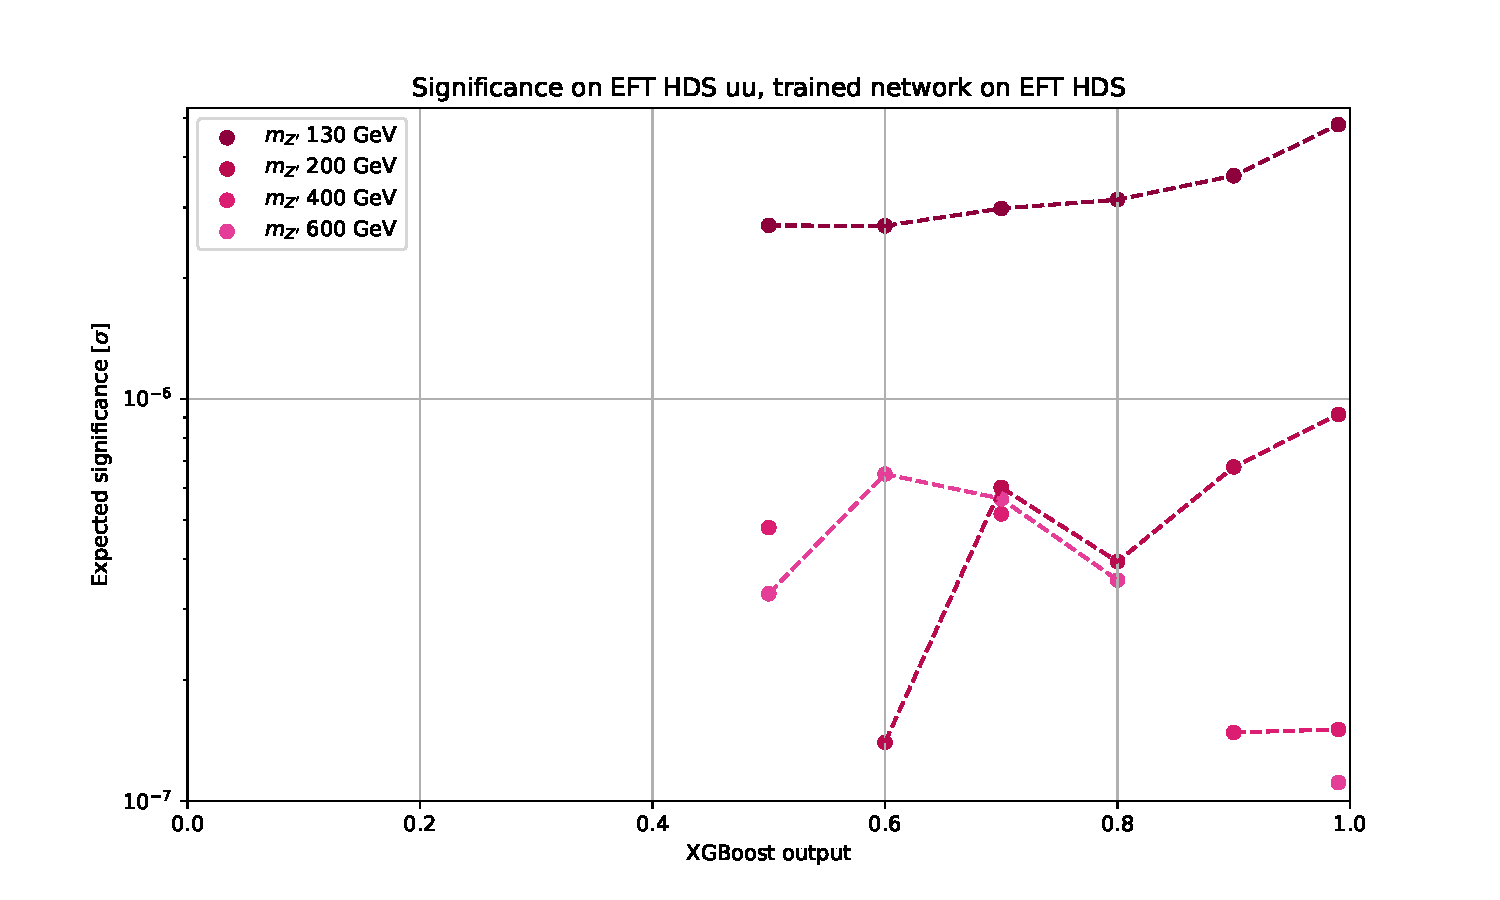
\includegraphics[width=1\textwidth]{XGBoost/EFT_HDS/EXP_SIG_uu.pdf}
      \end{subfigure}
   \caption{Expected significance plots for Z' mass points on network trained on Z' EFT HDS}\label{fig:EFT_HDS_exp_sig}
\end{figure}
\\Using the last bin as the significance is greatest there, such that we effectively make a cut based on the BDT score. Using the last bin, we can calculate a mass exclusion for both electron and muon channel.\\
\\To do so we need to count the number of signal and background events that are on the last bin, as well as their uncertainties. Aditionally we will include the number of real data events that are there such that we can follow the 
method explained in Chapter \ref{sec:stat_anal}. In Table \ref{tab:stat_vals_EFT_HDS} we see the values for each Z' mass point.
\begin{figure}[!ht]
	\centering
   \begin{subfigure}[b]{0.49\textwidth}
      \centering
      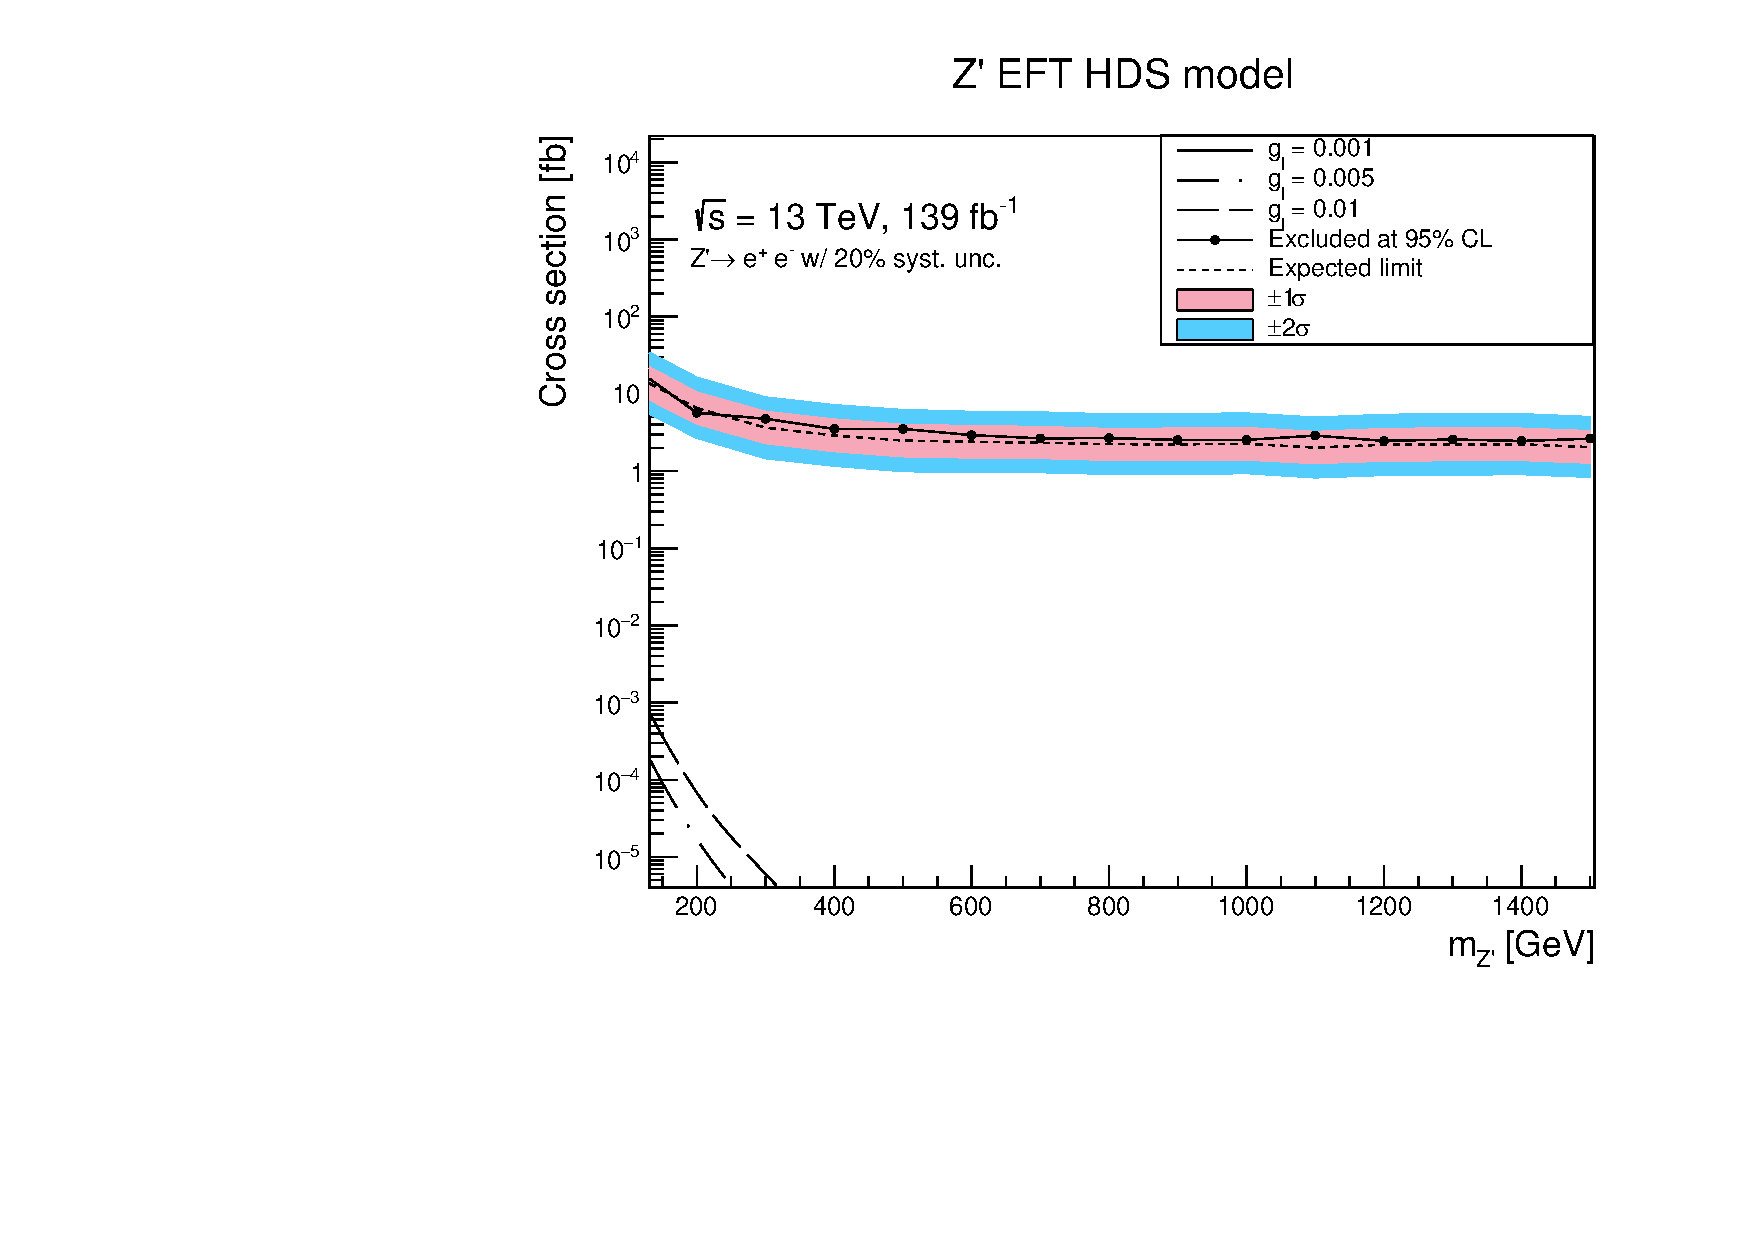
\includegraphics[width=1\textwidth]{Limits/EFT_HDS/mass_exclusion_ee.pdf}
      \end{subfigure}
   \hfill
   \begin{subfigure}[b]{0.49\textwidth}
      \centering
      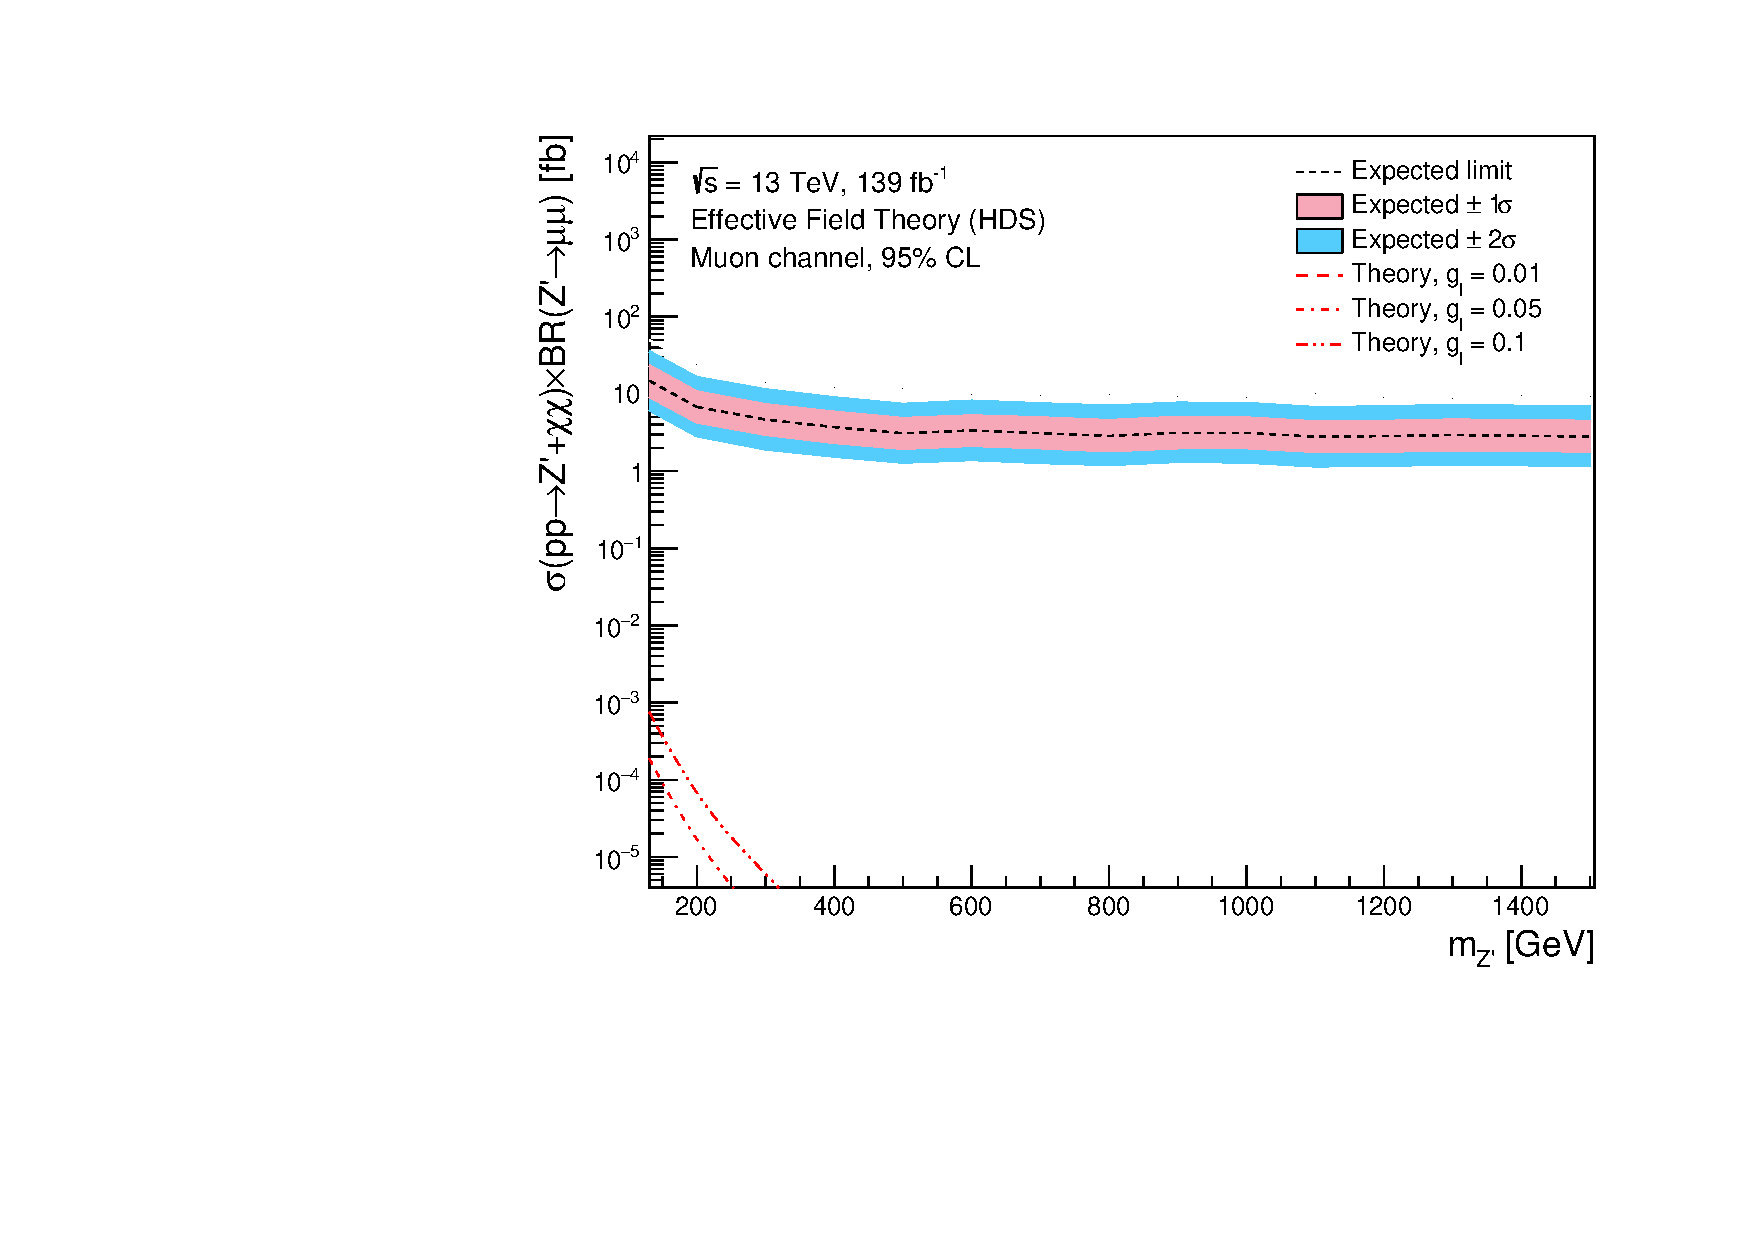
\includegraphics[width=1\textwidth]{Limits/EFT_HDS/mass_exclusion_uu.pdf}
      \end{subfigure}
   \caption{Mass exclusion limits of $ee$ and $\mu\mu$ channel for all Z' EFT HDS model}\label{fig:EFT_HDS_exclusion_ee_uu}
\end{figure}
As the lepton coupling was chosen to be $g_l=0.001$ when simulating the data, by the assumption that the number of events that survived the cuts is the same, we can increase this coupling to see how the mass limits changes.



\newpage
\section{Effective Field Theory Light Dark Sector}
Trained a network using all of the SM background samples and every different Z' mass of this model. Here are the results
% \begin{figure}[!ht]
% 	\centering
% 	\begin{subfigure}[b]{0.49\textwidth}
%       \centering
%       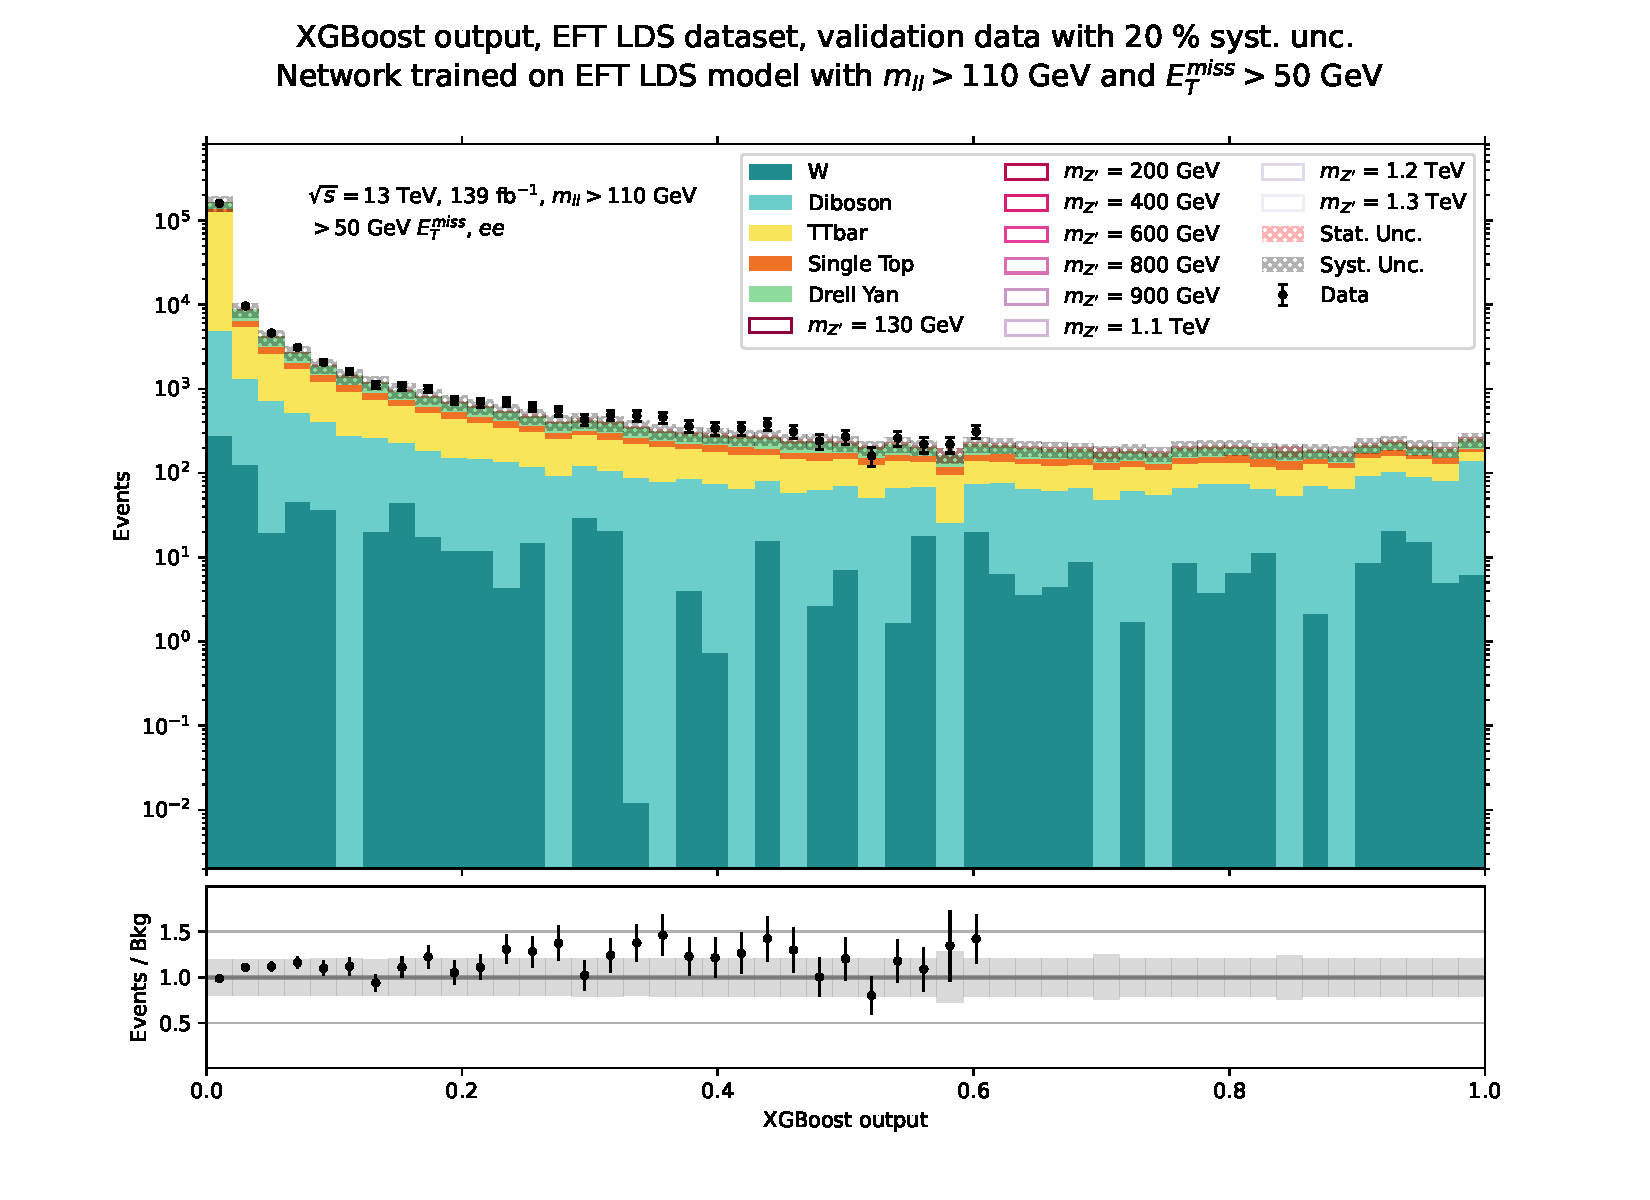
\includegraphics[width=1\textwidth]{XGBoost/EFT_LDS/VAL_ee.pdf}
%       \end{subfigure}
%    \hfill
%    \begin{subfigure}[b]{0.49\textwidth}
%       \centering
%       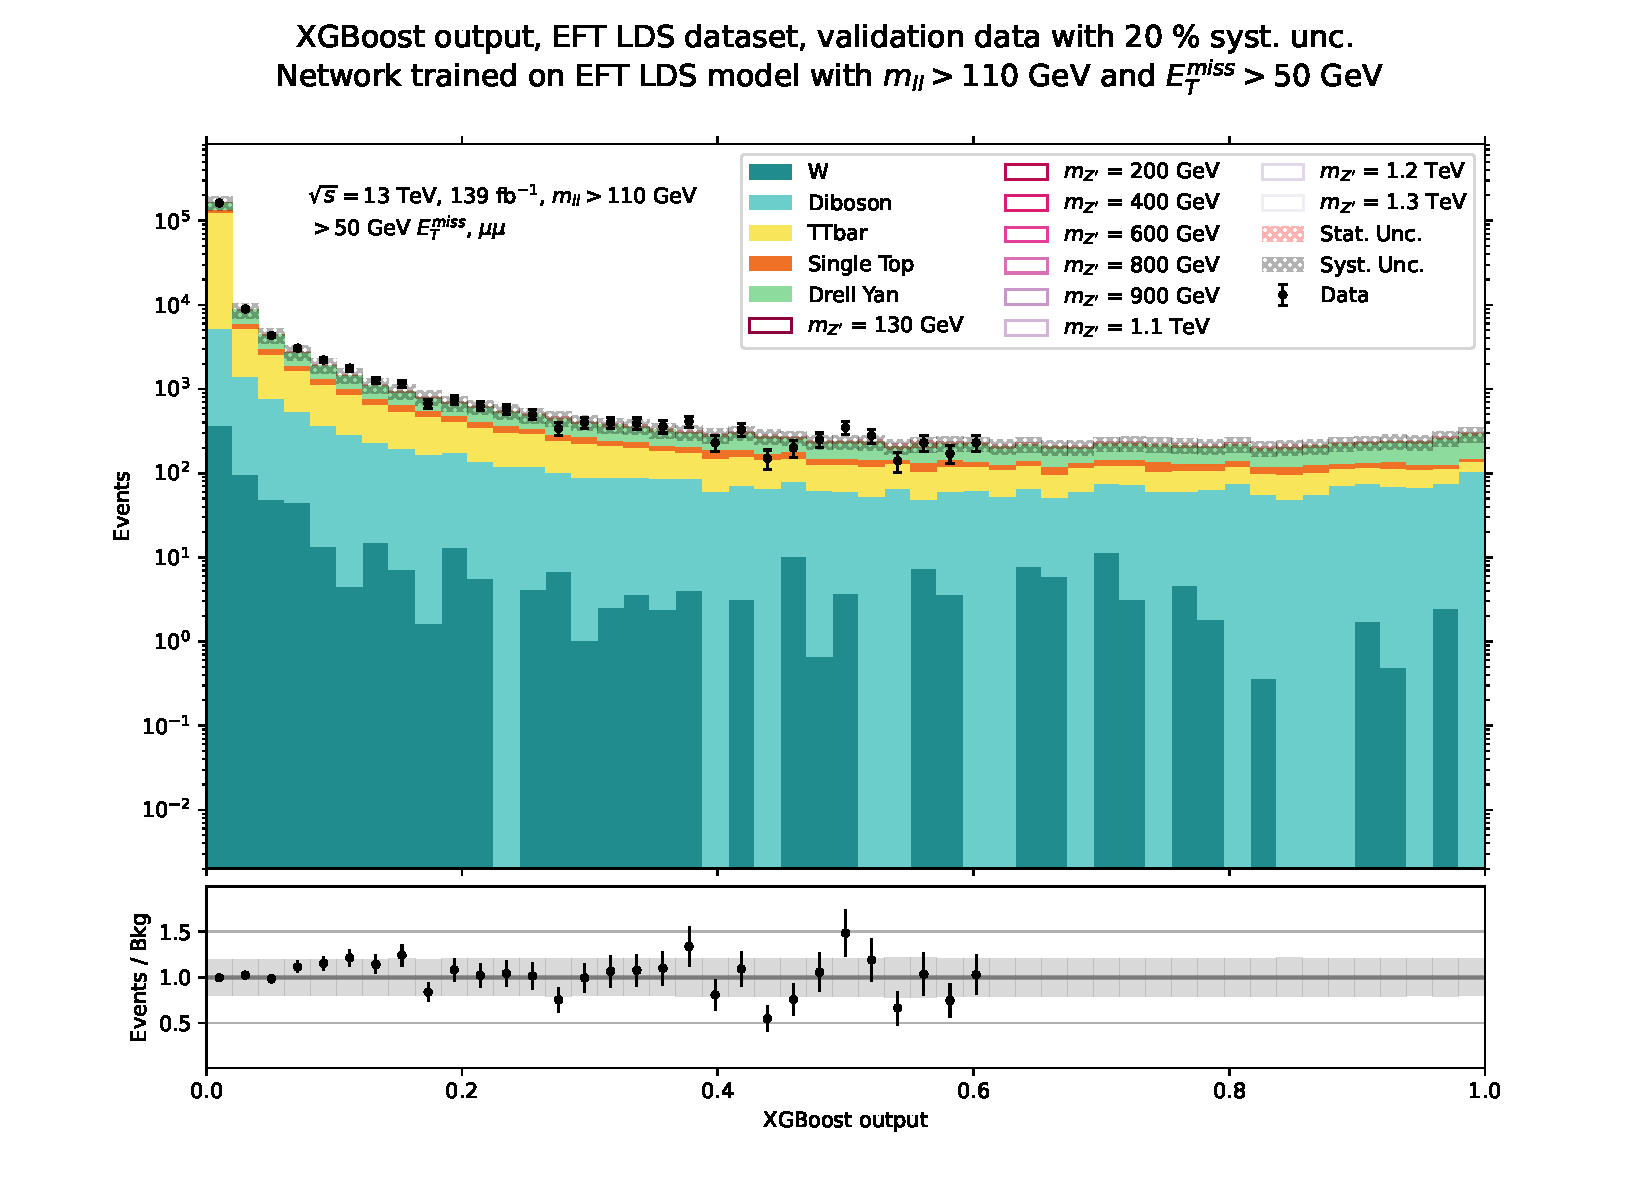
\includegraphics[width=1\textwidth]{XGBoost/EFT_LDS/VAL_uu.pdf}
%       \end{subfigure}
%    \caption{Validation plots for network trained on Z' EFT LDS}\label{fig:EFT_LDS_vals}
% \end{figure}
\\With the ROC for each mass point seen in Figure \ref{fig:EFT_LDS_ROCS}.
\begin{figure}[!ht]
	\centering
	\begin{subfigure}[b]{0.49\textwidth}
      \centering
      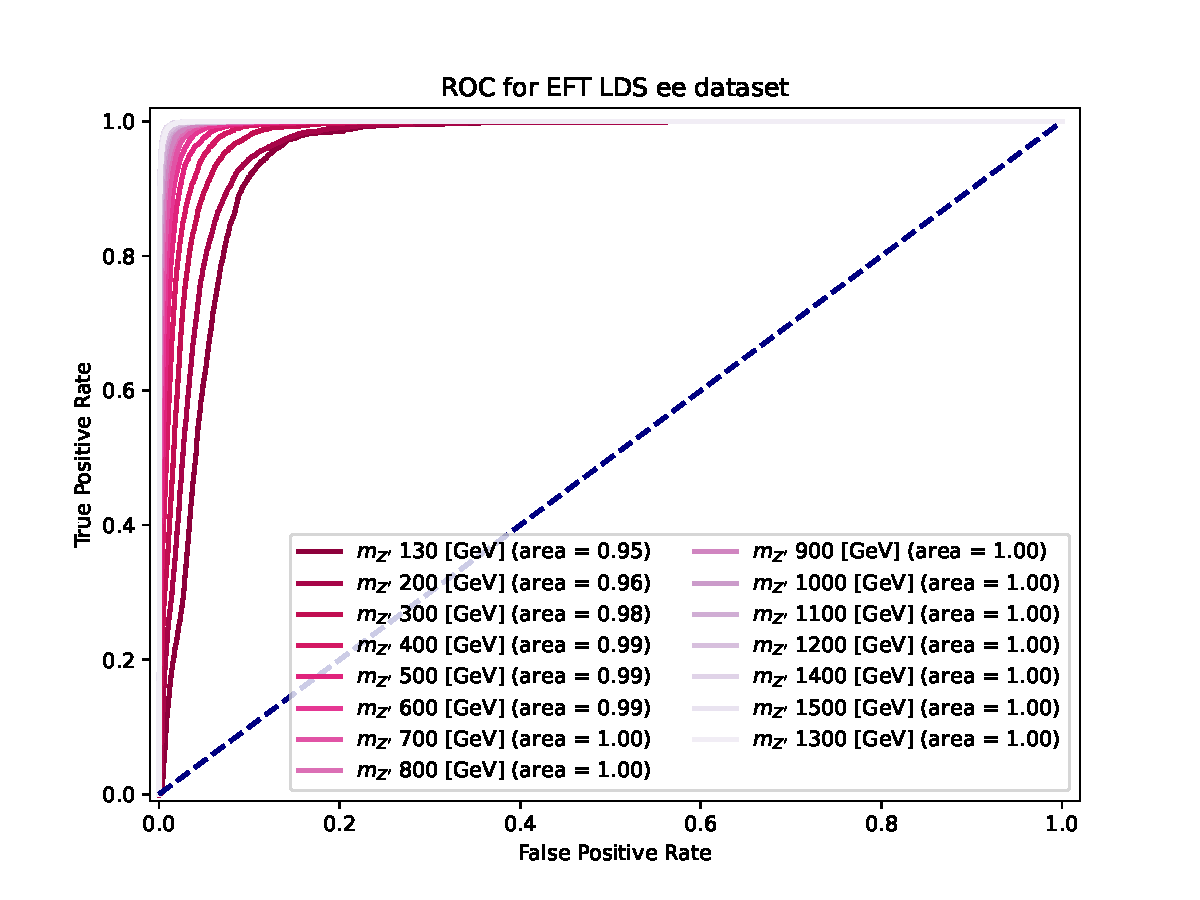
\includegraphics[width=1\textwidth]{XGBoost/EFT_LDS/ROC_ee.pdf}
      \end{subfigure}
   \hfill
   \begin{subfigure}[b]{0.49\textwidth}
      \centering
      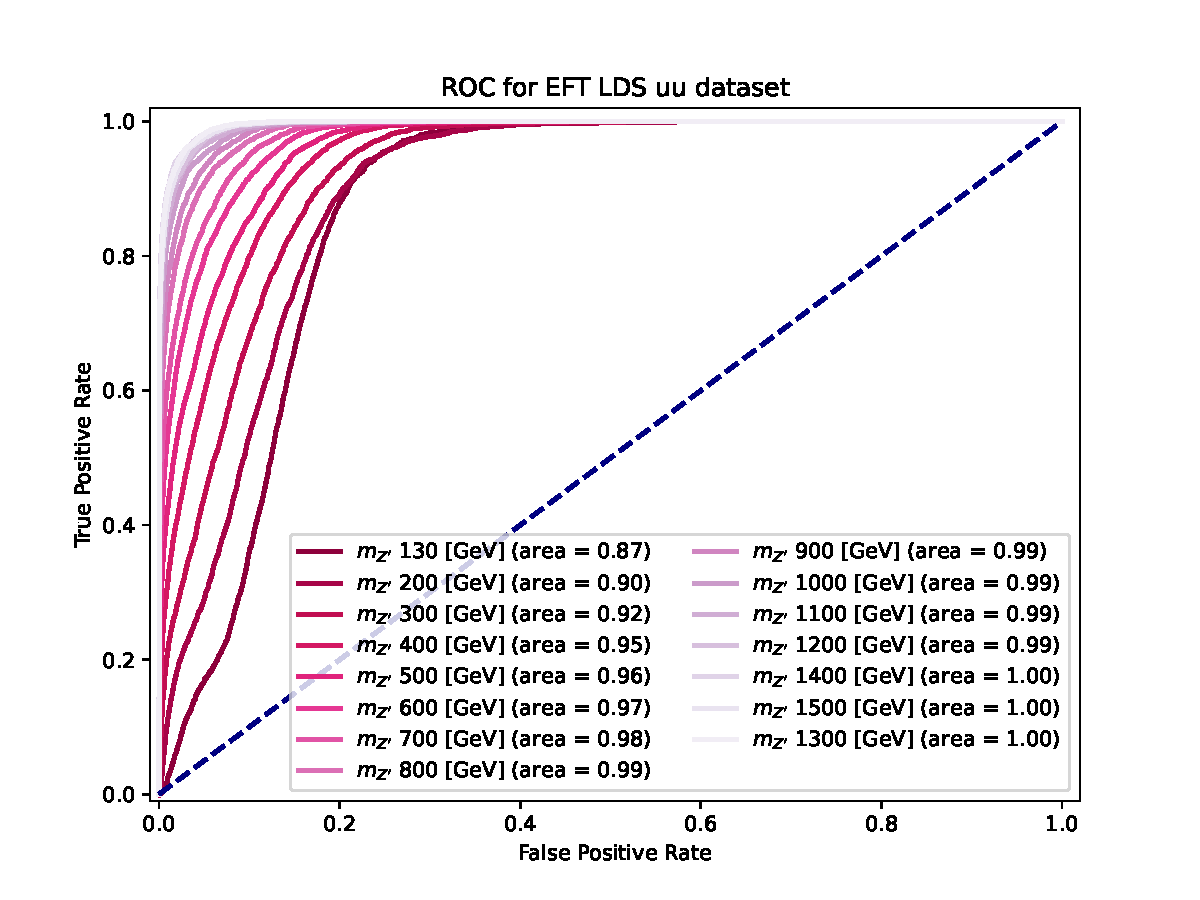
\includegraphics[width=1\textwidth]{XGBoost/EFT_LDS/ROC_uu.pdf}
      \end{subfigure}
   \caption{ROC plots for every Z' mass point on network trained on Z' EFT LDS}\label{fig:EFT_LDS_ROCS}
\end{figure}
\\Plotting the significance of the models given the binning we get the results from Figure \ref{fig:EFT_LDS_exp_sig}
\begin{figure}[!ht]
	\centering
	\begin{subfigure}[b]{0.49\textwidth}
      \centering
      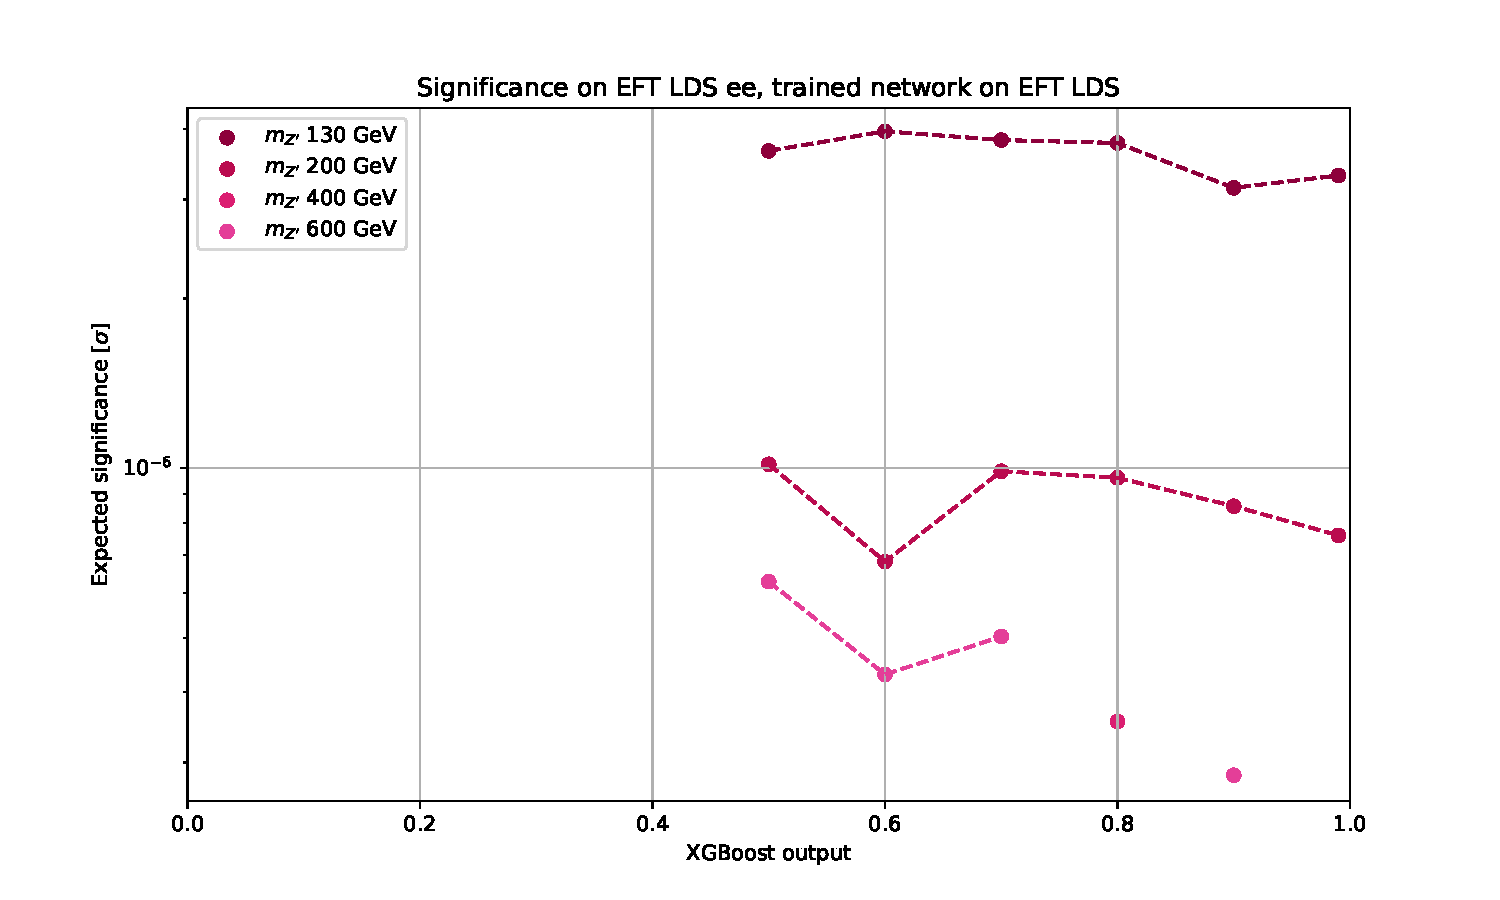
\includegraphics[width=1\textwidth]{XGBoost/EFT_LDS/EXP_SIG_ee.pdf}
      \end{subfigure}
   \hfill
   \begin{subfigure}[b]{0.49\textwidth}
      \centering
      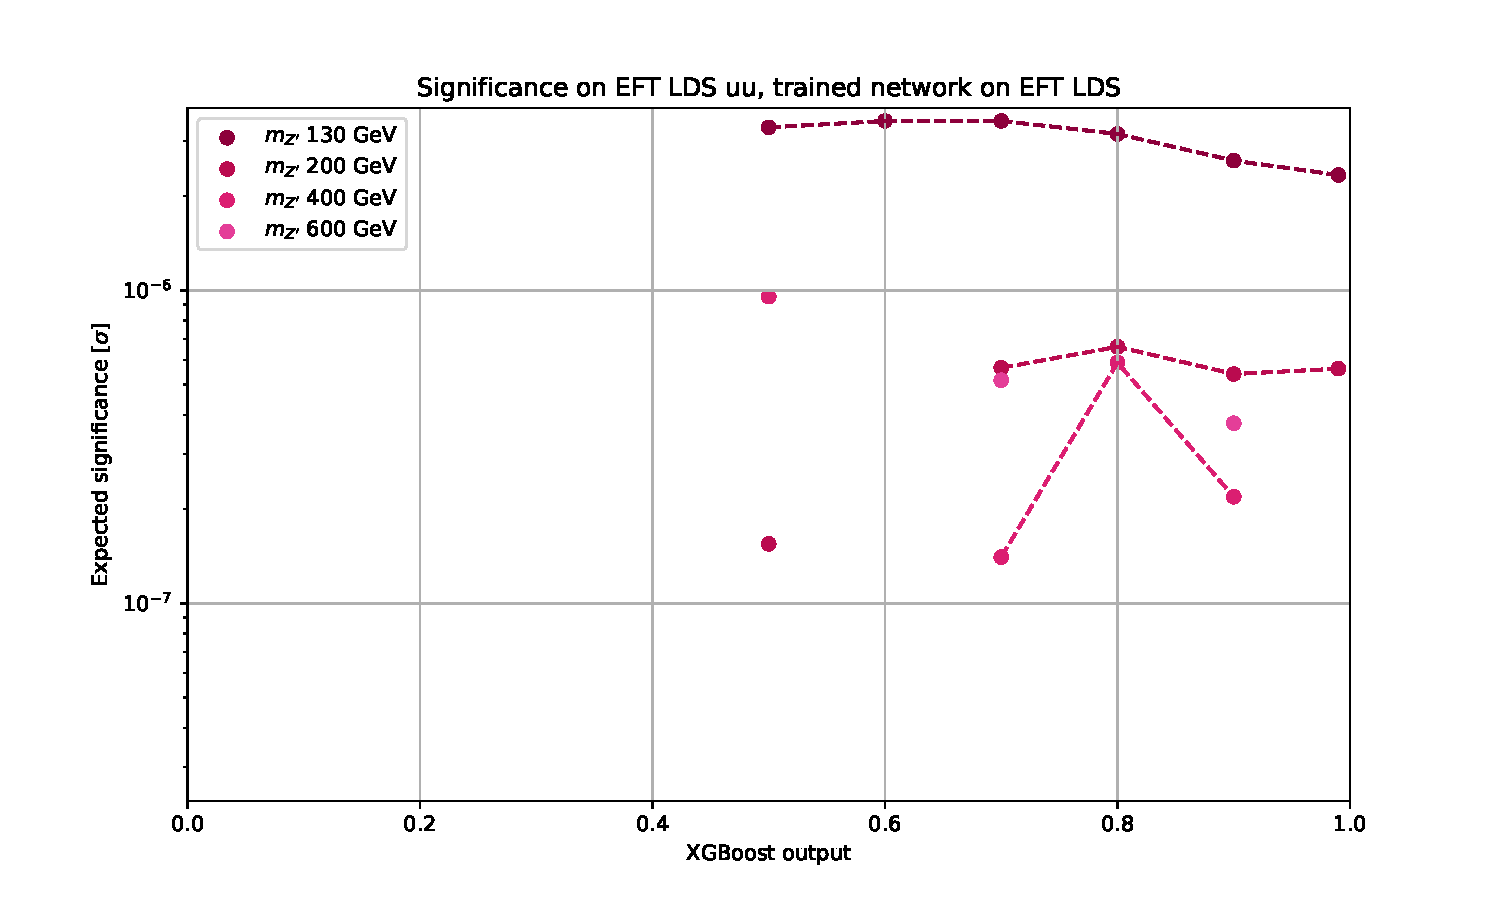
\includegraphics[width=1\textwidth]{XGBoost/EFT_LDS/EXP_SIG_uu.pdf}
      \end{subfigure}
   \caption{Expected significance plots for Z' mass points on network trained on Z' EFT LDS}\label{fig:EFT_LDS_exp_sig}
\end{figure}
\\Using the last bin as the significance is greatest there, such that we effectively make a cut based on the BDT score. Using the last bin, we can calculate a mass exclusion for both electron and muon channel.\\
\\To do so we need to count the number of signal and background events that are on the last bin, as well as their uncertainties. Aditionally we will include the number of real data events that are there such that we can follow the 
method explained in Chapter \ref{sec:stat_anal}. In Table \ref{tab:stat_vals_EFT_LDS} we see the values for each Z' mass point.
\begin{figure}[!ht]
	\centering
   \begin{subfigure}[b]{0.49\textwidth}
      \centering
      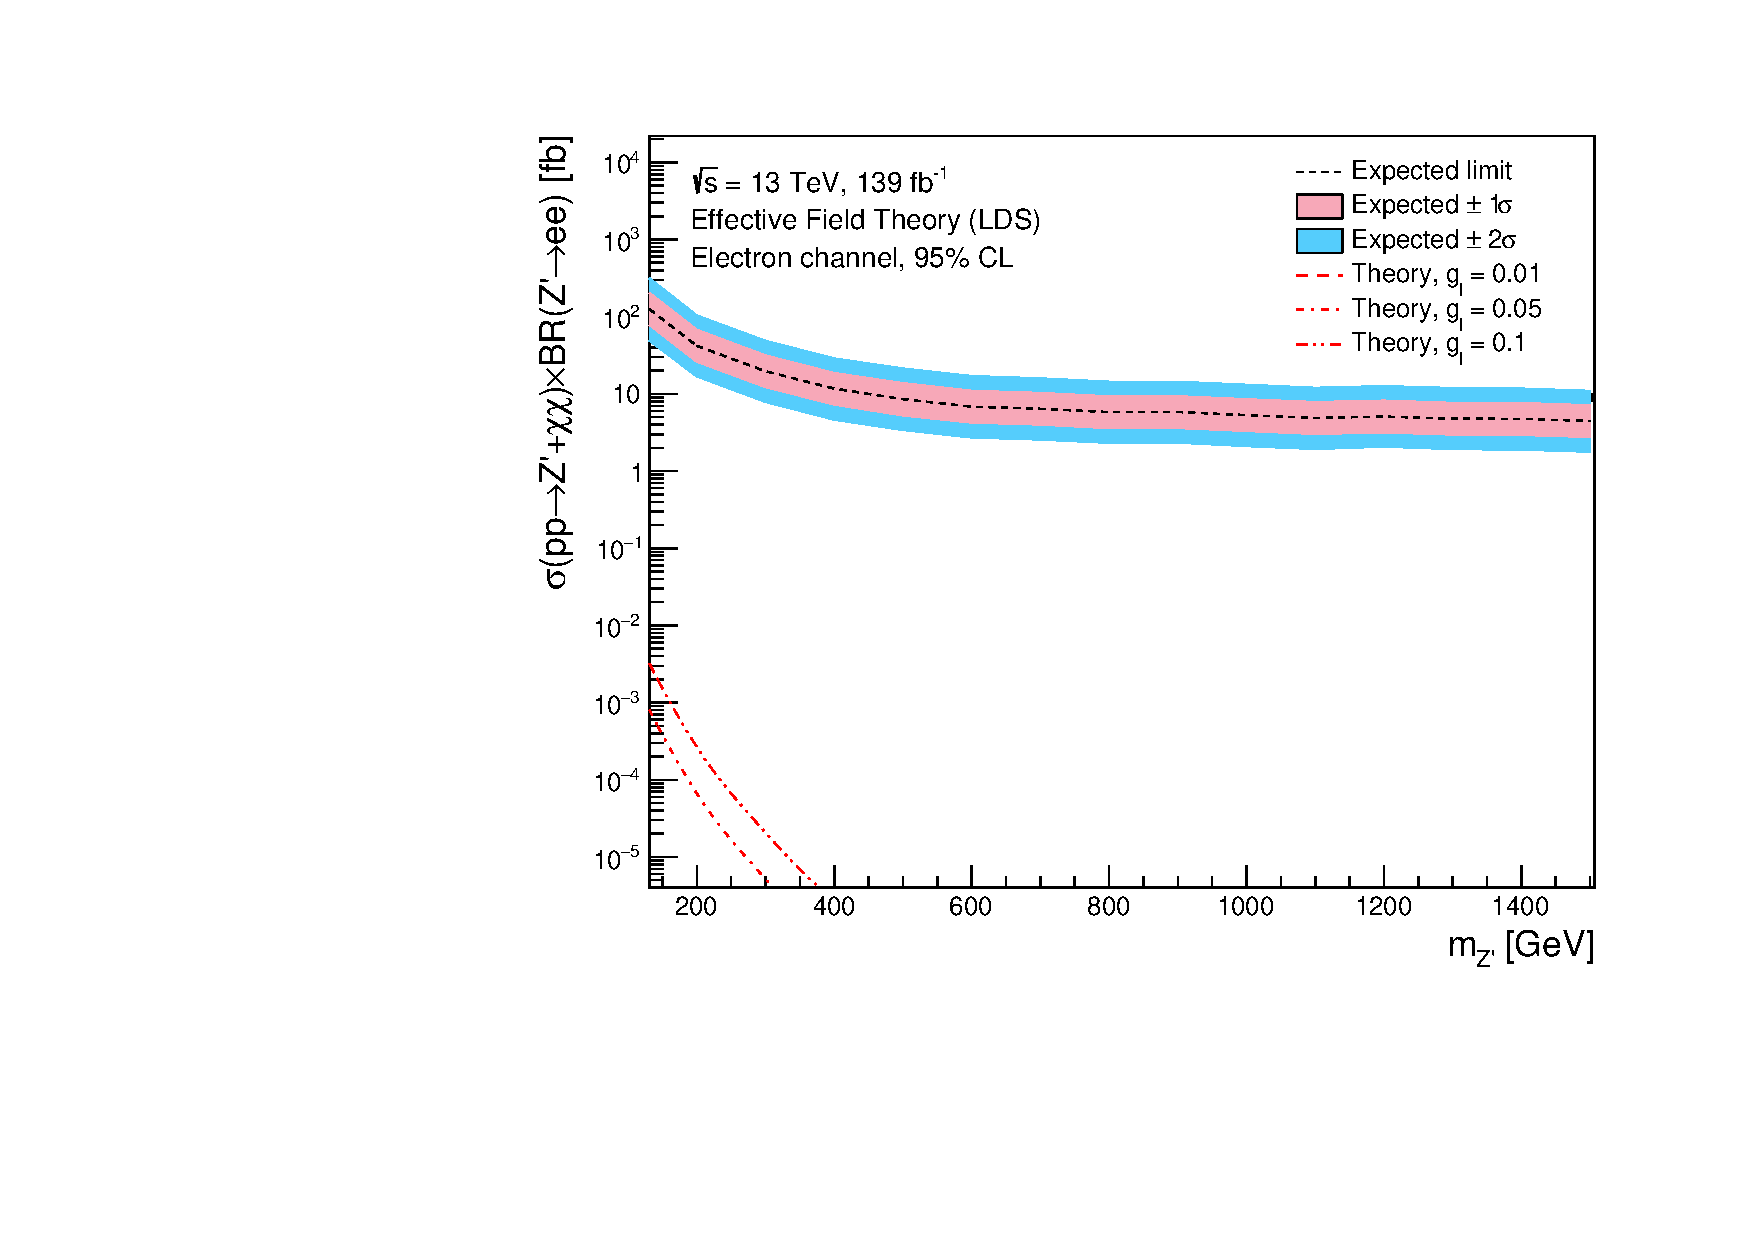
\includegraphics[width=1\textwidth]{Limits/EFT_LDS/mass_exclusion_ee.pdf}
      \end{subfigure}
   \hfill
   \begin{subfigure}[b]{0.49\textwidth}
      \centering
      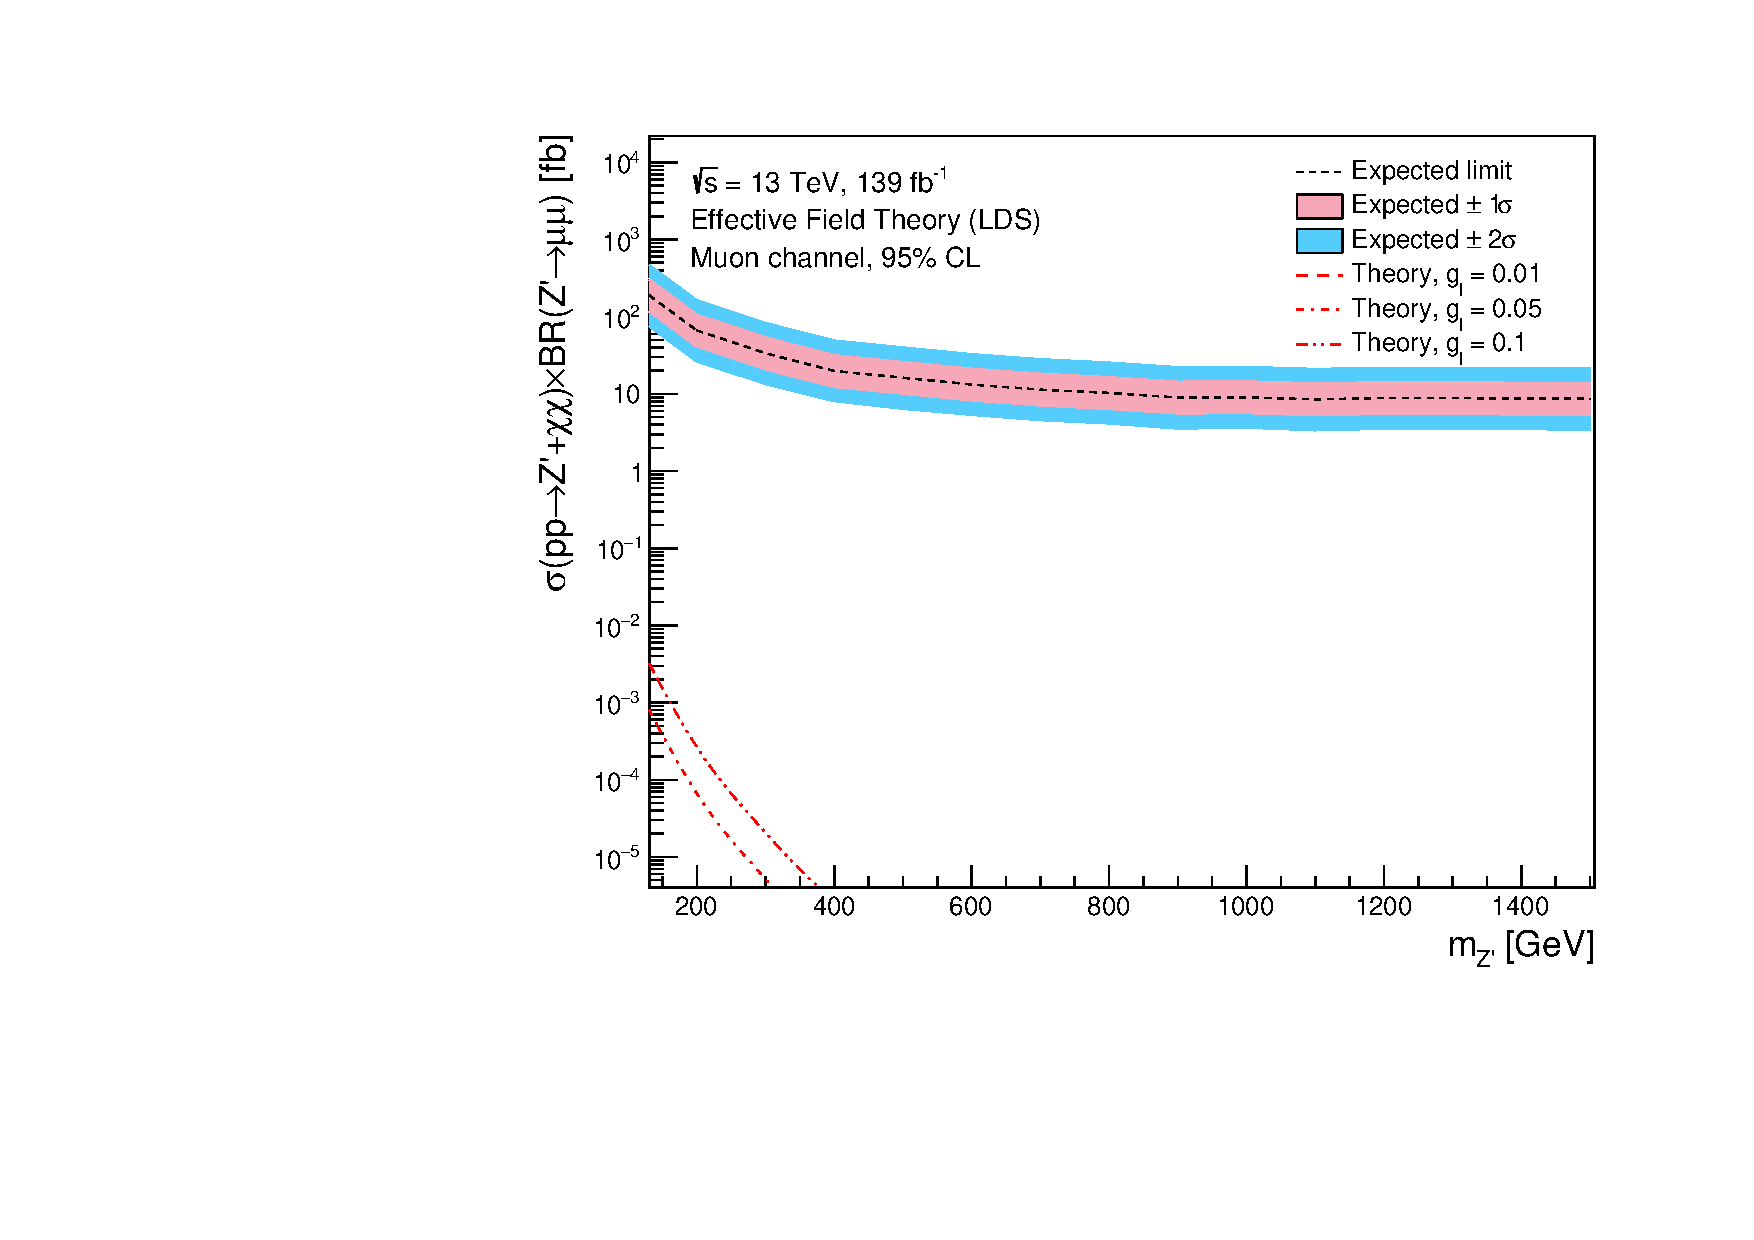
\includegraphics[width=1\textwidth]{Limits/EFT_LDS/mass_exclusion_uu.pdf}
      \end{subfigure}
   \caption{Mass exclusion limits of $ee$ and $\mu\mu$ channel for all Z' EFT LDS model}\label{fig:EFT_LDS_exclusion_ee_uu}
\end{figure}
As the lepton coupling was chosen to be $g_l=0.001$ when simulating the data, by the assumption that the number of events that survived the cuts is the same, we can increase this coupling to see how the mass limits changes.

\section{Mass exclusion limits for the combined channels}
\begin{figure}[!ht]
	\centering
	\begin{subfigure}[b]{0.49\textwidth}
      \centering
      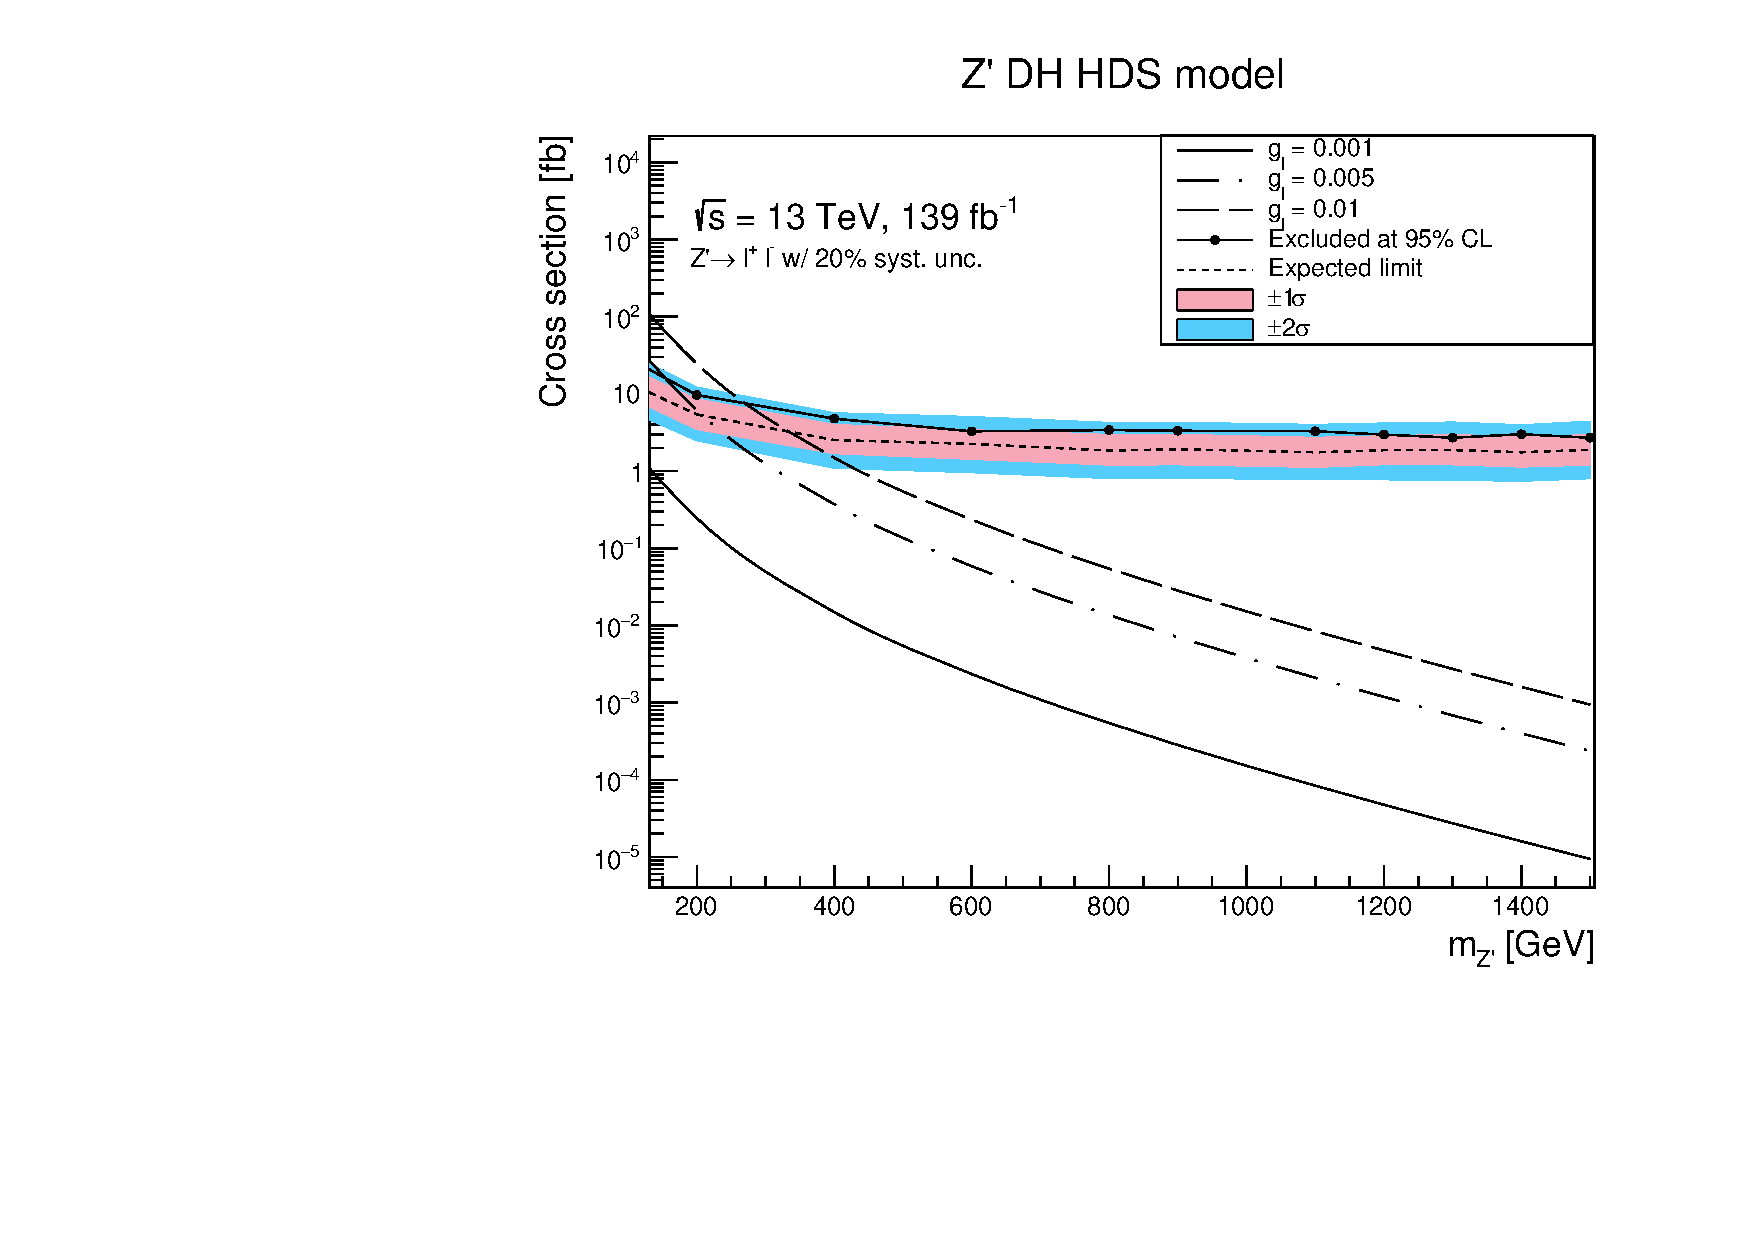
\includegraphics[width=1\textwidth]{Limits/DH_HDS/mass_exclusion_comb.pdf}
      % \caption{When including new variables and using 100 bins}
   \end{subfigure}
   \hfill
   \begin{subfigure}[b]{0.49\textwidth}
      \centering
      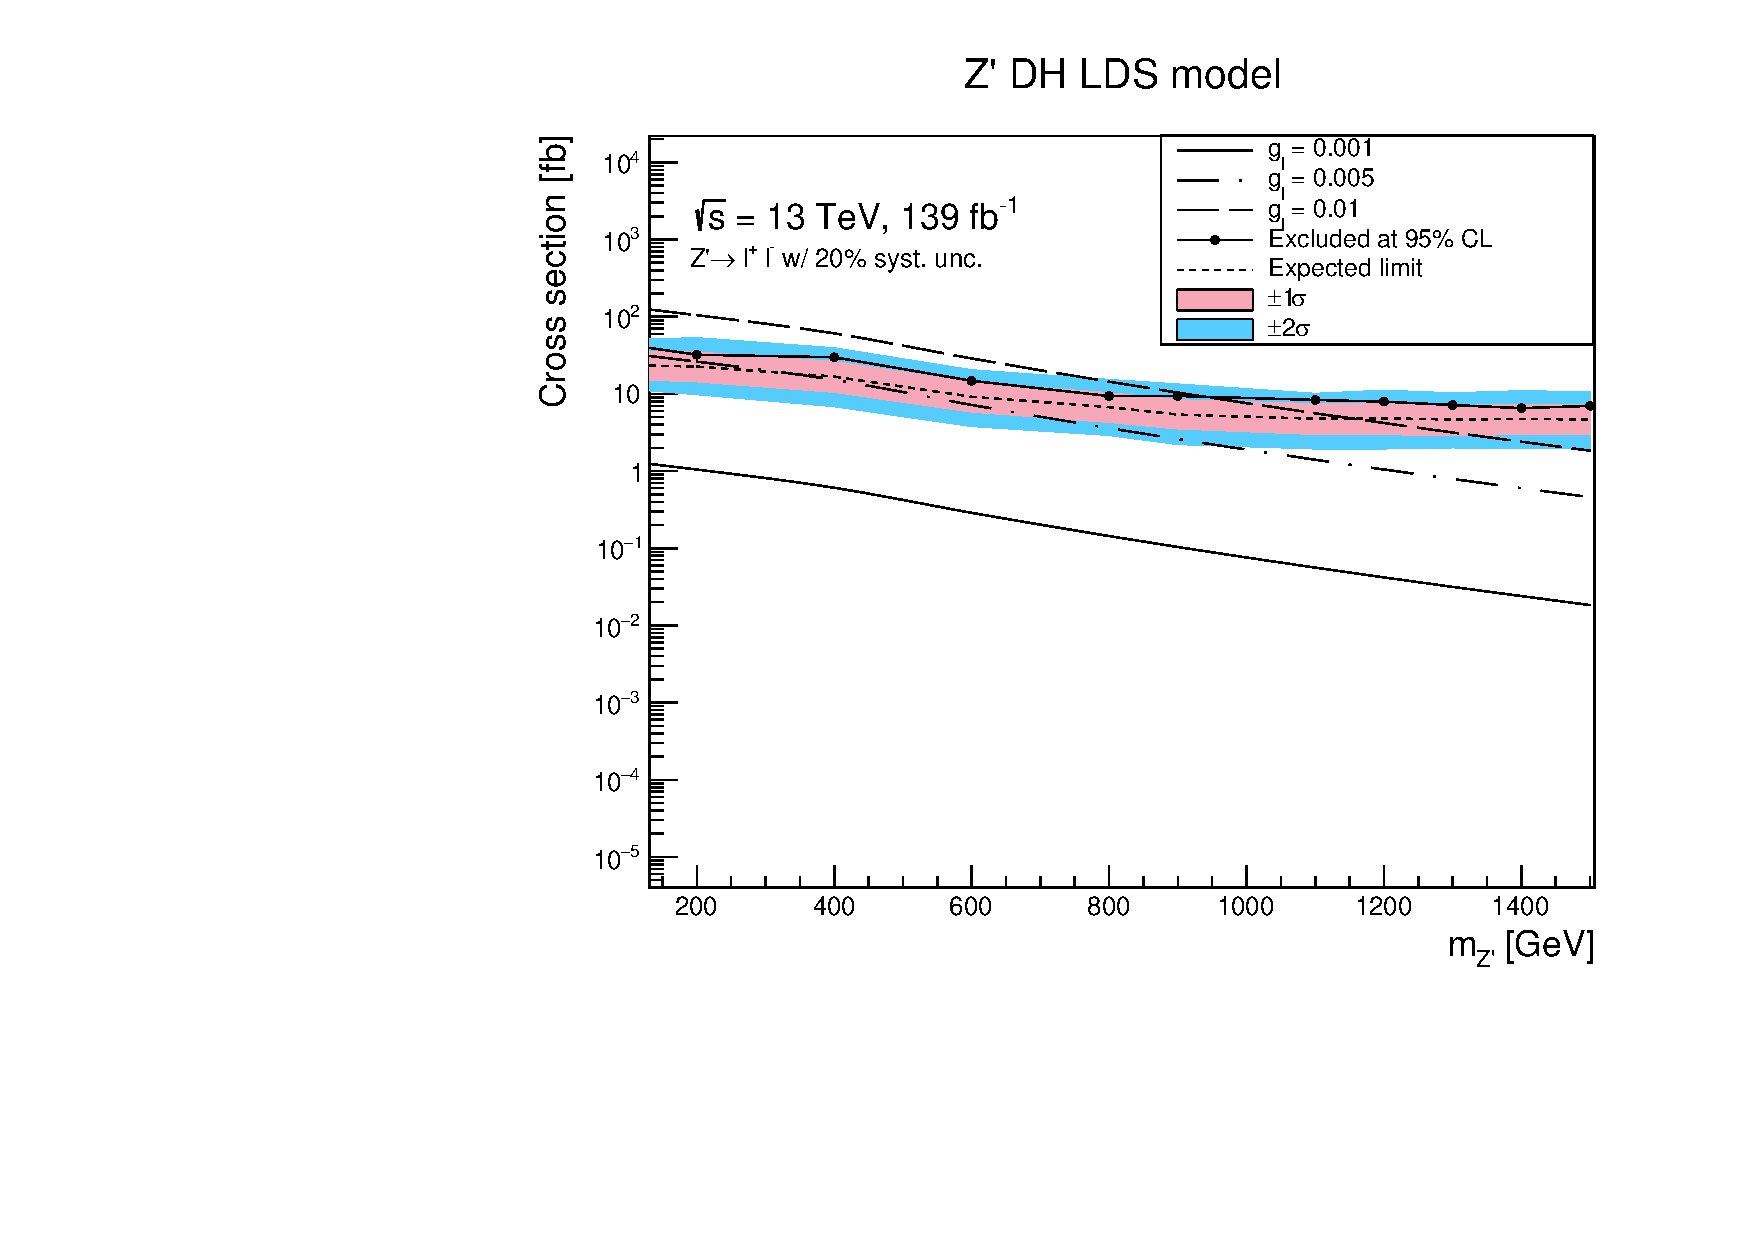
\includegraphics[width=1\textwidth]{Limits/DH_LDS/mass_exclusion_comb.pdf}
      % \caption{Expected significance of a)}
   \end{subfigure}
   \hfill
   \begin{subfigure}[b]{0.49\textwidth}
      \centering
      \includegraphics[width=1\textwidth]{Limits/LV_HDS/mass_exclusion_comb.pdf}
      % \caption{When including new variables and using 50 bins}
   \end{subfigure}
   \hfill
   \begin{subfigure}[b]{0.49\textwidth}
      \centering
      \includegraphics[width=1\textwidth]{Limits/LV_LDS/mass_exclusion_comb.pdf}
      % \caption{Expected significance of c)}
   \end{subfigure}
   \hfill
	\begin{subfigure}[b]{0.49\textwidth}
      \centering
      \includegraphics[width=1\textwidth]{Limits/EFT_HDS/mass_exclusion_comb.pdf}
      % \caption{When excluding new variables and using 50 bins}
   \end{subfigure}
   \hfill
   \begin{subfigure}[b]{0.49\textwidth}
      \centering
      \includegraphics[width=1\textwidth]{Limits/EFT_LDS/mass_exclusion_comb.pdf}
      % \caption{Expected significance of e)}
   \end{subfigure}
   \caption[Mass exclusion limits of combined $ee$ and $\mu\mu$ channel for all models]{Mass exclusion limits of combined $ee$ and $\mu\mu$ channel for all models}\label{fig:model_dep_exclusions}
\end{figure}
\clearpage

\end{document}